\documentclass[a4j , 11pt , twoside]{jbook}
\usepackage{ascmac} % プログラムリスト等を囲むボックスのため
\usepackage{matx} % MaTXのロゴ(例)「\MaTX{}を用いた制御系設計」
\usepackage{manyfloat} % 1ページに多くの図や表をまとめるため
\usepackage{here} % 画像を好きな位置に配置できる
\usepackage{docmute}
\usepackage{amsmath}
\usepackage{ascmac} 
\usepackage{fancybox}
\usepackage[dvipdfmx]{graphicx}% ポストスクリプトファイルを取り込むため
\usepackage{url}
\usepackage{color}
\usepackage{moreverb}
\begin{document}
%-----------------------------------------------------------
% タイトルページ
\title{倒立振子の安定化制御}
\author{渡部僚太}
\date{2018年7月2日}
\maketitle
%-----------------------------------------------------------
% 目次
\pagenumbering{roman} %ページ番号をローマ数字に設定
\tableofcontents % 目次
\listoffigures % 図の目次
\listoftables % 表の目次
\cleardoublepage % 次ページが表ページになるように改ページ
\pagenumbering{arabic} % ページ番号をアラビア数字に設定
%-----------------------------------------------------------------
% 本文
\chapter{TODOリスト}
	\section{理解}
16日(日曜日)と17日(月曜日)を前段階\\
18日(火曜日)を本段階\\
19日(水曜日)と20日(木曜日)を後段階\\
それ以降をデッドラインと命名する

\section{進捗}
%-------------------------------------------------------------------
	\subsection{それ以前}
		\begin{itemize}
		  \item レポートの日付を変える---後段階
		  \item TODOリストを消す---後段階
		\end{itemize}
%-------------------------------------------------------------------
	\subsection{はじめに}
		\begin{itemize}
		  \item 参考文献の[1]はどうするか---本段階
		  \item 倒立振子系の実際の写真を載せる---本段階
		  \item 図の訂正---後段階
		  \item 文章の訂正および修正---後段階
		\end{itemize}
%-------------------------------------------------------------------
	\subsection{モデリング}
		\begin{itemize}
		  \item 図の訂正(MaTX生成の.epsファイルは位置がおかしいので要訂正)---後段階(できれば本段階)
		  \item 文章の訂正および修正---後段階
		  \item Mとfのフィードバックによる測定の仕方を間違えているのでもう一度実験しなおしデータを再取得する---本段階
		\end{itemize}
%-------------------------------------------------------------------
	\subsection{制御系設計}
		\begin{itemize}
		  \item 文章の訂正および修正---後段階
		  \item 図の訂正(特にする必要はないと思うが)---後段階
		\end{itemize}
%-------------------------------------------------------------------
	\subsection{シミュレーション}
		\begin{itemize}
		  \item 文章の訂正および修正---後段階
		  \item 図の訂正---後段階
		  \item 「振り上げ制御及び安定化に対する制御性能評価」を完成させる
		  \begin{itemize}
		    \item 表が変なところにいく問題を解決---前段階★
		    \item 考察しやすいシミュレーション3パターンの画像を用意する---できるなら前段階★
		   	\item 考察をかく---本段階(できるなら前段階)★
		  \end{itemize}
		\end{itemize}
%-------------------------------------------------------------------
	\subsection{実験}
		\begin{itemize}
		  \item 文章の訂正および修正---後段階
		  \item 図の訂正---後段階
		  \item 「目標値変更実験」を完成させる
		   \begin{itemize}
		     \item 12パターンの実験を行い直す---本段階
		     \item シミュレーションの考察がお萎える図を作成---本段階
		     \item シミュレーション結果と実験結果を描画した図を作成---本段階
		     \item 結果と考察を述べる---本段階
		  \end{itemize}
		  \item 「振り上げ制御及び安定化実験」を完成させる
		  	\begin{itemize}
		  	  \item 3パターンの実験を行いなおす---本段階
		  	  \item シミュレーションの考察が行える図を作成---本段階
		  	  \item シミュレーション結果と実験結果を描画した図を作成---本段階
		  	  \item 結果と考察を述べる---本段階
		  	\end{itemize}
		\end{itemize}
%-------------------------------------------------------------------
	\subsection{おわりに}
		\begin{itemize}
		  \item 文章自体を考え直す---後段階
		  \item 他に書くことはないか---後段階
		\end{itemize}
%-------------------------------------------------------------------
	\subsection{参考文献}
		\begin{itemize}
		  \item 参考文系DBを完成させる---後段階
		  \item 参考文献を本文中に挿入する---後段階
		\end{itemize}
%-------------------------------------------------------------------
	\subsection{プログラム}
		\begin{itemize}
		  \item 長いソースコードだと改ページされない問題を解決する---前段階★
		\end{itemize}
%-------------------------------------------------------------------

\chapter{はじめに}
	\section{これは節}
\section{これも節}
\chapter{モデリング}
	\section{倒立振子のモデリング}
実験目的を達成する制御システムを設計するためにまず、倒立振子系について、状態方程式と観測方程式から成る数式モデルを導出する。
\subsection{状態方程式}
	\begin{figure}[H]
		\centering
		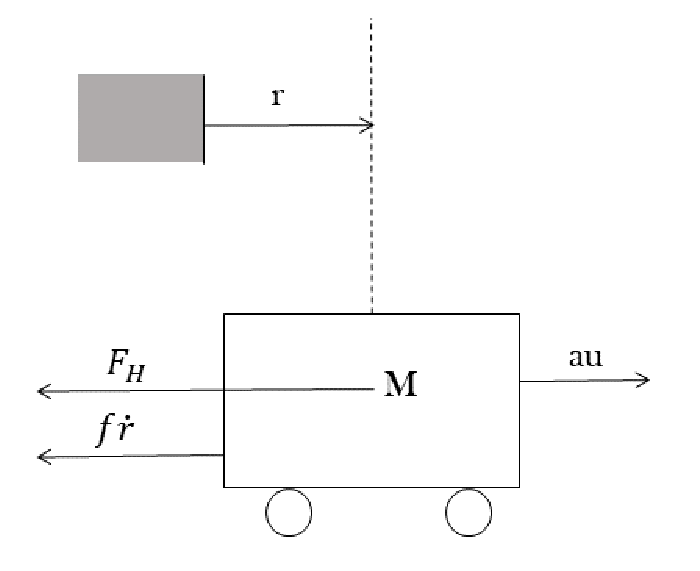
\includegraphics[width=0.4\linewidth]{gazo/cart.eps}
		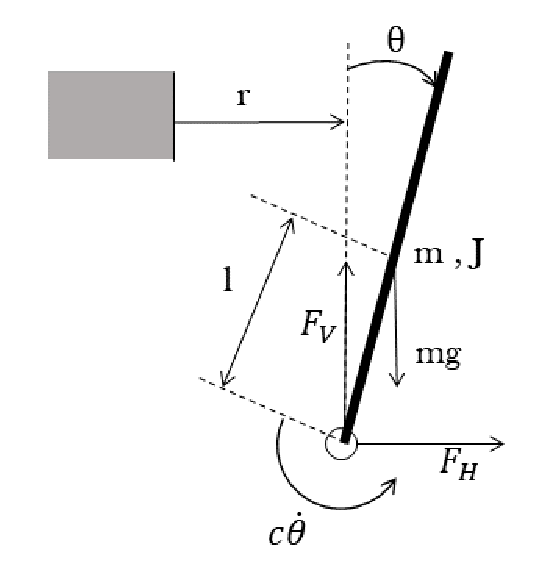
\includegraphics[width=0.4\linewidth]{gazo/stick.eps}
		\caption{数式モデル導出のための参考図}
		\label{image:reference}
	\end{figure}	
	図\ref{image:reference}を参考に各運動方程式を導出すると、\\
	台車の運動方程式は\\
	
	\begin{equation}
		M\ddot{r}=au-F_{H}-f\dot{r}
		\label{eq:motion_eq_cart}
	\end{equation}
	
	倒立振子の回転の運動方程式は
	
	\begin{equation}
		J\ddot{\theta}=lF_{V}\sin \theta -lF_{H}\cos \theta -c\dot{\theta}
		\label{eq:rotemotion_eq_stick}
	\end{equation}
	\\
	倒立振子の水平方向の運動方程式は
	
	\begin{equation}
		m\frac{d^{2}}{dt^{2}}(r+l\sin\theta) = F_{H}
		\label{eq:horizonmotion_eq_stick}
	\end{equation}
	倒立振子の垂直方向の運動方程式は
	
	\begin{equation}
		m\frac{d^{2}}{dt^{2}}(l\cos\theta) = F_{V}-mg
		\label{eq:vertical_eq_stick}
	\end{equation}
	
	となる。
	\par
	ここで各式の導出過程を述べる。図\ref{image:reference}より台車の運動方程式は、振り子からの水平抗力$F_{H}$を考慮してニュートンの第二法則より(\ref{eq:motion_eq_cart})
	式を導くことができる。
	ただし、$M$は台車の質量、$f$は台車の摩擦係数、$a$は駆動アンプへの入力電圧から台車への駆動までのゲイン、$u$はモータの駆動アンプへの入力電圧、$r$は台車の基準位置からの変位である。
	同様にニュートンの第二法則を用いることでそれぞれの方向における(\ref{eq:horizonmotion_eq_stick}),(\ref{eq:vertical_eq_stick})式の運動方程式を導くことができる。
	ただし、$m$は振り子の質量、$l$は回転軸・重心間の距離、$g$は重力加速度、$F_{V}$は振り子が台車から受ける垂直抗力である。
	また、$\theta$は鉛直上向きを$\theta=0$としたときの角度である。
	\par
	最後に(\ref{eq:rotemotion_eq_stick})式は回転に対する運動方程式を考えることで上記と同様に求めることができる。
	ただし、$J$は重心回りの慣性モーメント、$c$は回転軸摩擦係数である。
	\par
	いま、4つの状態変数から成るベクトル、すなわち状態$x$を
					
	\[
		x=\left[
		\begin{array}{ccc}
			r\\
			\theta\\
			\dot{r}\\
			\dot{\theta}\\
		\end{array}
		\right]
		\label{eq:array1}
	\]
					
	のように定義し、(\ref{eq:motion_eq_cart})式,(\ref{eq:rotemotion_eq_stick})式,(\ref{eq:horizonmotion_eq_stick})式,(\ref{eq:vertical_eq_stick})式
	から倒立振子系の非線形状態方程式を求める。
	
	\begin{eqnarray}
		\dot{x} = f(x,u) = \left[
		\begin{array}{ccc}
			\dot{r}\\
			\dot{\theta}\\
			\ddot{r}\\
			\ddot{\theta}\\
		\end{array}
		\right]
		\label{eq:array2}
	\end{eqnarray}
					
	ここで(\ref{eq:horizonmotion_eq_stick})式より$F_{H}$を、
	(\ref{eq:vertical_eq_stick})式より$F_{V}$を求めると
	
	\begin{align}
		F_{H} &= m\frac{d^{2}}{dt^{2}}r + ml\frac{d^{2}}{dt^{2}}\sin{\theta} \notag \\
		&= m\ddot{r}+ml(-\dot{\theta}^{2}\sin{\theta}+\ddot{\theta}\cos{\theta})
		\label{eq:eq1}
	\end{align}
	
	\begin{align}
		F_{V} &= mg + m\frac{d^{2}}{dt^{2}}(l\cos{\theta}) \notag \\
		&= mg + ml(-\dot{\theta}^{2}\cos{\theta}-\ddot{\theta}\sin{\theta})
		\label{eq:eq2}
	\end{align}
	
	である。\\
	(\ref{eq:eq1})式を(\ref{eq:motion_eq_cart})式に代入すると
	
	\begin{equation}
		(M+m)\ddot{r} + ml\ddot{\theta}\cos{\theta}-ml\dot{\theta}^{2}\sin{\theta}+f\dot{r}=au
		\label{eq:eq3}
	\end{equation}
	
	である。\\
	(\ref{eq:eq1})式と(\ref{eq:eq2})式を(\ref{eq:rotemotion_eq_stick})式に代入すると
	
	\begin{equation}
		(J + ml^{2})\ddot{\theta} + ml\ddot{r}\cos{\theta} - mgl\sin{\theta} + c\dot{\theta} = 0
		\label{eq:eq4}
	\end{equation}
	
	である。\\
	(\ref{eq:eq3})式、(\ref{eq:eq4})式を行列表現すると
	
	\[
		\left[
		\begin{array}{ccc}
			(M + m)\ddot{r} + (ml\cos{\theta})\ddot{\theta} + (-ml\sin{\theta}) + f\dot{r} = au \\
			(ml\cos{\theta})\ddot{r} + (J + ml^{2})\ddot{\theta} -mgl\sin{\theta} + c\dot{\theta} = 0\\
		\end{array}
		\right]
	\]
	
	\[
		\left[
		\begin{array}{ccc}
			M + m & ml\cos{\theta} \\
			ml\cos{\theta} & J + ml^{2}\\
		\end{array}
		\right]
		\left[
		\begin{array}{ccc}
			\ddot{r} \\
			\ddot{\theta}\\
		\end{array}
		\right] +
		\left[
		\begin{array}{ccc}
			-ml\ddot{\theta}^{2}\sin{\theta} + f\dot{r}\\
			mgl\sin{\theta} + c\dot{\theta}\\
		\end{array}
		\right] = 
		\left[
		\begin{array}{ccc}
			au\\
			0\\
		\end{array}
		\right]
	\]
	
	$\begin{pmatrix} M + m & ml\cos{\theta} \\ ml\cos{\theta} & J + ml^{2} \end{pmatrix}$を$K$と置いて右辺に逆行列としてかけると\\
	
	\[
		\left[
		\begin{array}{ccc}
			\ddot{r}\\
			\ddot{\theta}\\
		\end{array}
		\right]=K^{-1}
		\left[
		\begin{array}{ccc}
			au-f\dot{r}+ml\ddot{\theta}\sin{\theta}\\
			mgl\sin{\theta} - c\dot{\theta}\\
		\end{array}
		\right]
	\]
	\\
	よって以上から(\ref{eq:array2})式は\\
	
	\begin{equation}
		\dot{x} = f(x,u)=\left[
		\begin{array}{ccc}
			\dot{r}\\
			\dot{\theta}\\
			K^{-1}\left[
			\begin{array}{ccc}
				-f\dot{r}+ml\ddot{\theta}\sin{\theta}+au\\
				mgl\sin{\theta}-c\dot{\theta}
			\end{array}
			\right]
		\end{array}
		\right]
		\label{eq:array3}
	\end{equation}
	\\
	となる。ただし、$K$は
	
	\begin{equation}
		K=\left[
		\begin{array}{ccc}
			M+m & ml\cos{\theta}\\
			ml\cos{\theta} & J+ml^{2}\\
		\end{array}
		\right]
		\label{eq:array4}
	\end{equation}
	
	である。
	よって倒立振子系の非線形状態方程式は(\ref{eq:array3})式のように得られる。
	\par
	ところで、倒立振子系については、その制御目的から、不安定平衡点$x=0$の近傍での挙動を表す
	状態方程式を知れば十分である。そこで、この基準状態まわりで一時近似された状態方程式を求め
	ることを考える。\\
	(\ref{eq:array3})式に一次近似のテイラー展開を施すと、\\
	\begin{equation}
		f(x,u) = f(0,0) + \left.\frac{\partial f}{\partial x}\right|_{x=0,u=0}(x-0) + \left.\frac{\partial f}{\partial u}\right|_{x=0,u=0}(u-0)
		\label{eq:eq4}
	\end{equation}
	\\
	となる。つまり、(\ref{eq:eq4})を計算すれば求めたい状態方程式を得ることができる。\\
	(\ref{eq:eq4})式において、
	
	\[A=\left.\frac{\partial f}{\partial x}\right|_{x=0,u=0} , B=\left.\frac{\partial f}{\partial u}\right|_{x=0,u=0}\]
	
	とすると、(\ref{eq:eq4})式は以下のように計算できる。
	\begin{equation}
		f(x,u) = Ax+Bu
		\label{eq:AxBu}
	\end{equation}
	ここで、一時近似を施したので、$\theta$を微小範囲と考えることができ、\\ $\sin{\theta} \simeq  \theta , \cos{\theta} \simeq 1 , \dot{\theta}^{2} \simeq 0$のように
	近似できる。\\
	以上の近似から(\ref{eq:array3}),(\ref{eq:array4})式は\\
	\begin{equation}
		f(x,u)=\left[
		\begin{array}{ccc}
			\dot{r}\\
			\dot{\theta}\\
			K^{'-1}\left[
			\begin{array}{ccc}
				au-f\dot{r}\\
				mlg\theta-c\dot{\theta}\\
			\end{array}
			\right]
		\end{array}
		\right]
		\label{eq:array5}
	\end{equation}
	
	\begin{equation}
		K^{'} = \left[
		\begin{array}{ccc}
			M + m & ml\\
			ml & J+ml^{2}\\
		\end{array}
		\right]
		\label{eq:array6}
	\end{equation}
	
	となる。ここで、(\ref{eq:array5})式の3行目を$a_{1}$と置き、4行目を$a_{2}$と置く。\\\newpage
	(\ref{eq:array5})、(\ref{eq:array6})式を用いて(\ref{eq:AxBu})式のA、Bを計算する。\\
	
	\begin{align*}
		A=\frac{\partial \textgt{f}}{\partial \textgt{x}}&=
		\left[
		\begin{array}{cccc}
			\frac{\partial \dot{r}}{\partial r} & \frac{\partial \dot{r}}{\partial \theta} & \frac{\partial \dot{r}}{\partial \dot{r}} & \frac{\partial \dot{r}}{\partial \dot{\theta}} \\
			\frac{\partial \dot{\theta}}{\partial r} & \frac{\partial \dot{\theta}}{\partial \theta} & \frac{\partial \dot{\theta}}{\partial \dot{r}} & \frac{\partial \dot{\theta}}{\partial \dot{\theta}} \\
			\frac{\partial a_{1}}{\partial r} & \frac{\partial a_{1}}{\partial \theta} & \frac{\partial a_{1}}{\partial \dot{r}} & \frac{\partial a_{1}}{\partial \dot{\theta}} \\
			\frac{\partial a_{2}}{\partial r} & \frac{\partial a_{2}}{\partial \theta} & \frac{\partial a_{2}}{\partial \dot{r}} & \frac{\partial a_{2}}{\partial \dot{\theta}} \\
		\end{array} 
		\right]  \\
		&=\left[
		\begin{array}{cccc}
			0 & 0 & 1 & 0 \\
			0 & 0 & 0 & 1 \\
			0 & 0 & K^{'-1}(-f) & 0\\
			0 & K^{'-1}(mgl) & 0 & K^{'-1}(-c) \\
		\end{array}
		\right]
	\end{align*}
	\\
	\[
		B=\frac{\partial \textgt{f}}{\partial \textgt{u}}=
		\left[
		\begin{array}{c}
			\frac{\partial \dot{r}}{\partial u}\\
			\frac{\partial \dot{\theta}}{\partial u}\\
			\frac{\partial a_{1}}{\partial u}\\
			\frac{\partial a_{2}}{\partial u}\\
		\end{array}
		\right]=
		\left[
		\begin{array}{c}
			0\\
			0\\
			K^{'-1}a\\
			0\\
		\end{array}
		\right]
		\label{eq:array7}
	\]
	\\
	以上から線形状態方程式は\\
	\[\dot{x}=A\textgt{x}+B\textgt{u}\]
	\begin{equation}
		=\left[
		\begin{array}{cccc}
			0 & 0 & 1 & 0 \\
			0 & 0 & 0 & 1 \\
			0 & 0 & K^{'-1}(-f) & 0 \\
			0 & K^{'-1}(mgl) & 0 & K^{'-1}(-c)\\
		\end{array}
		\right]
		\left[
		\begin{array}{c}
			r\\
			\theta\\
			\dot{r}\\
			\dot{\theta}\\
		\end{array}
		\right] + 
		\left[
		\begin{array}{c}
			0\\
			0\\
			K^{'-1}au\\
			0\\
		\end{array}
		\right]
		\label{eq:InPeAboveLiner}
	\end{equation}
	\\
	となる。ただし、$K^{'}$は(\ref{eq:array6})式である。上式の線形状態方程式は鉛直上向きを$\theta = 0$としたときの状態方程式である。
	鉛直下向きを$\theta = 0$とした場合は(\ref{eq:array4})式の三角関数内の
	$\theta$に+$\pi$すればよいので
	\begin{equation}
		\dot{x} = f(x,u)=\left[
		\begin{array}{ccc}
			\dot{r}\\
			\dot{\theta}\\
			K^{-1}\left[
			\begin{array}{ccc}
				-f\dot{r}-ml\ddot{\theta}\sin{\theta}+au\\
				-mgl\sin{\theta}-c\dot{\theta}
			\end{array}
			\right]
		\end{array}
		\right]
		\label{eq:InPeUnderNonLiner}
	\end{equation}
	\\
	となる。ただし、$K$は
	\begin{equation}
		K=\left[
		\begin{array}{ccc}
			M+m & -ml\cos{\theta}\\
			-ml\cos{\theta} & J+ml^{2}\\
		\end{array}
		\right]
		\label{eq:InPeUnderNonLinerK}
	\end{equation}
	である。\\
	振子の角度を鉛直上向きを$\theta=0$としたときの状態方程式を線形化したときと同様に
	(\ref{eq:InPeUnderNonLiner}),(\ref{eq:InPeUnderNonLinerK})式を線形化すると
	線形状態方程式は\\
	\[\dot{x}=A\textgt{x}+B\textgt{u}\]
	\begin{equation}
		=\left[
		\begin{array}{cccc}
			0 & 0 & 1 & 0 \\
			0 & 0 & 0 & 1 \\
			0 & 0 & K^{'-1}(-f) & 0 \\
			0 & K^{'-1}(-mgl) & 0 & K^{'-1}(-c)\\
		\end{array}
		\right]
		\left[
		\begin{array}{c}
			r\\
			\theta\\
			\dot{r}\\
			\dot{\theta}\\
		\end{array}
		\right] + 
		\left[
		\begin{array}{c}
			0\\
			0\\
			K^{'-1}au\\
			0\\
		\end{array}
		\right]
		\label{eq:InPeUnderLiner}
	\end{equation}
	\\
	となる。ただし、$K$は、
	\[
		K=\left[
		\begin{array}{ccc}
			M+m & -ml\\
			-ml & J+ml^{2}\\
		\end{array}
		\right]
	\]
	である。\\
	今後、(\ref{eq:InPeAboveLiner})式を鉛直上向き基準の線形状態方程式とし、
	(\ref{eq:InPeUnderLiner})式を鉛直下向き基準の線形状態方程式とする。
	
\subsection{観測方程式}
	2つの観測出力は
	\[
		y_{1} = c_{1}r\\
	\]
	\[
		y_{2} = c_{2}\theta\\
	\]
	のように表される。ここで、$c_{1}$は変位・電圧変換係数、$c_{2}$は角度・電圧変換係数である。これから成るベクトル出
	力$y$を\\
	\[
		y=\left[
		\begin{array}{c}
			y_{1}\\
			y_{2}\\
		\end{array}
		\right]
	\]
	のように定義すると、倒立振子系に対する観測方程式として\\
	\begin{align}
		y&=Cx \notag \\
		\left[
		\begin{array}{c}
			y_{1}\\
			y_{2}\\
		\end{array}
		\right]&=\left[
		\begin{array}{cccc}
			c_{1} & 0 & 0 & 0 \\
			0 & c_{2} & 0 & 0\\
		\end{array}
		\right]\left[
		\begin{array}{c}
			r\\
			\theta\\
			\dot{r}\\
			\dot{\theta}\\
		\end{array}
		\right]
		\label{eq:output}
	\end{align}
	を得ることができる。\\
	なお、鉛直上向きを基準とした場合でも鉛直下向きを基準とした場合でも出力方程式は変わらない。
%一次チェック完了:
%----------------------------------------------------------------------------------------------------
\section{倒立振子のパラメータの同定}
数式モデル(\ref{eq:array6})、(\ref{eq:array7})、(\ref{eq:output})に含まれる物理パラメータを実際の倒立振子系で実験
を行い同定する。
\subsection{mとlの測定}
	倒立振子系から振子を取り外し、バネ秤で振子の質量$m$を測定する。つぎに、振子を鋼尺のエッジ上でバランス
	させて、重心の位置を定め、$l$を測定する。
	以下に測定した結果を示す。
	\[m = 0.031[\rm{kg}]\]
	\[l = 0.15[\rm{m}]\]
\subsection{aの測定}
	モータに一定電圧を加え、ばねばかりで台車を引き、台車が正の方向に動き出すときの力($au+摩擦力$)を$f_{max}$
	、負の方向に動き出すときの力($au-摩擦力$)を$f_{min}$とする。図\ref{image:parameterA}に示すように
	$u$と$f_{max},f_{min}$の関係をいくつかの電圧について調べ、最小2乗法によって1次関数を求め、この傾きを
	$a$とする。\cite{Koga:Binpe}
	\begin{figure}[H]
		\centering
		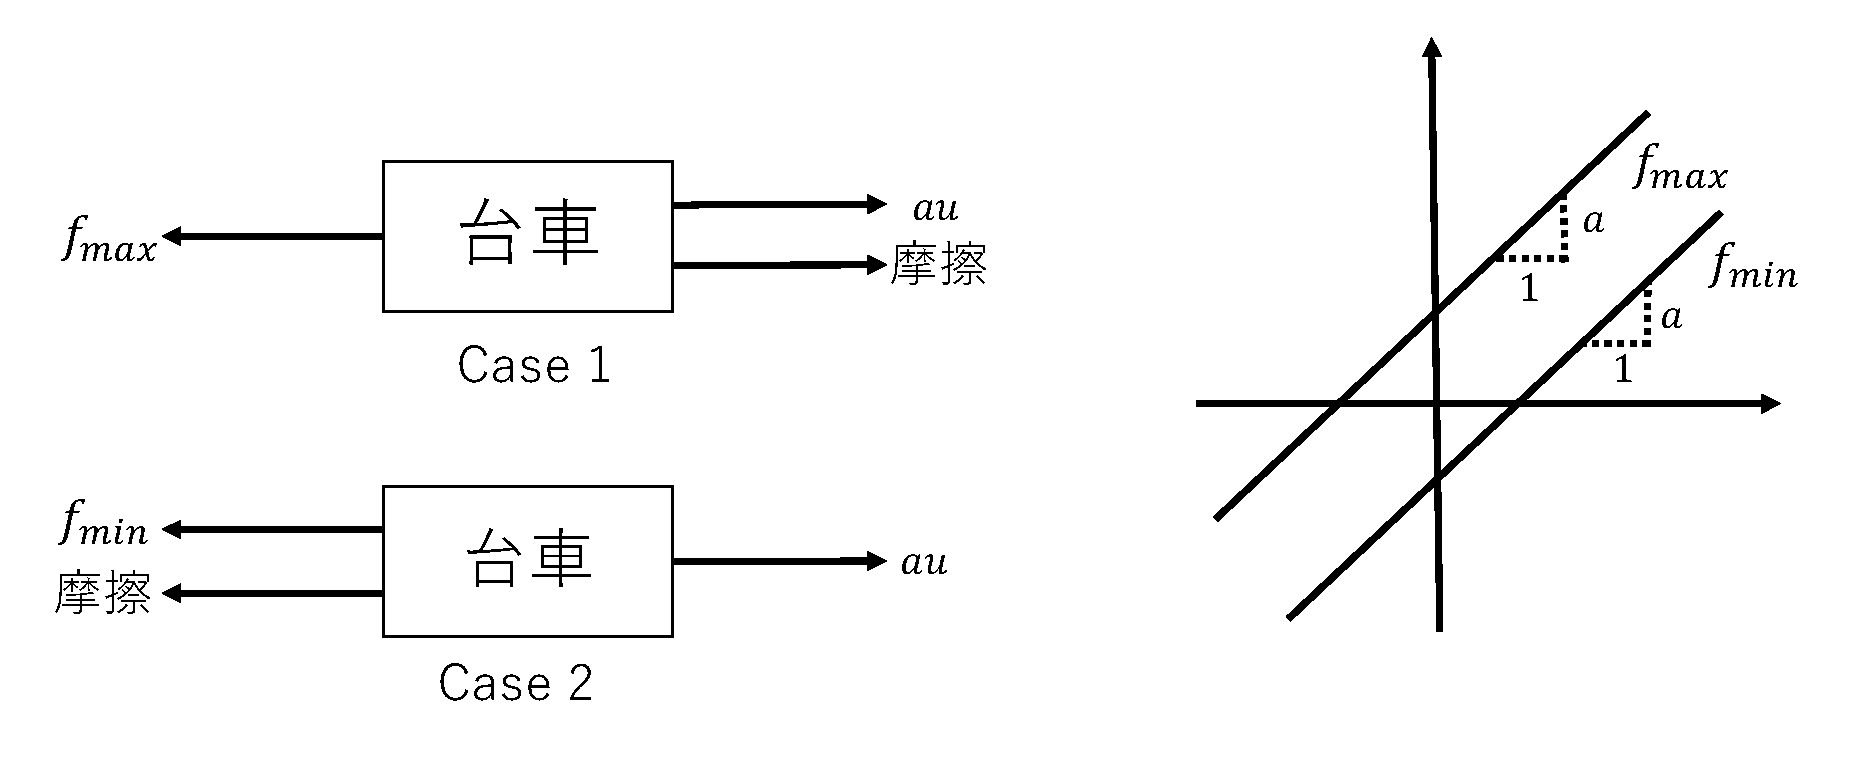
\includegraphics[width=1.0\linewidth]{gazo/ParameterA.eps}
		\caption{パラメータaの決定}
		\label{image:parameterA}
	\end{figure}
	なお、振子は台車から取り外して測定を行う。
	以下に測定した結果から得られた一次関数の傾き$a$を示す。
	\[
		a=0.062[\rm{Kg/V}] = 0.61[\rm{N/V}
	]\]
	
\subsection{Jとcの測定}
	振子を自由振動させることにより、$J$と$c$を測定できる。その数式モデルは鉛直下向きを基準として
	\begin{equation}
		(J + ml^{2})\ddot{\theta} - mgl\sin{\theta} + c\dot{\theta} = 0
		\label{eq:Para1}
	\end{equation}
	\begin{equation}
		y_{2} = c_{2}\theta
	\label{eq:Para2}
	\end{equation}
	で与えられる。$\theta$を微小範囲で考えると、(\ref{eq:Para1}),(\ref{eq:Para2})式は
	\[
		\ddot{y}_{2} + 2\zeta\omega_{n}\dot{y}_{2} + \omega_{n}^{2}y_{2} = 0
	\]
	ただし、
	\[
		\zeta = \frac{c}{2\sqrt{mgl\left(J + ml^{2}\right)}} 
		,\ \  \omega_{n} = \sqrt{\frac{mgl}{J+ml^{2}}}
	\]
	のように書くことができる。この解は
	\[0<\zeta<1\]
	のとき、減衰振動となり
	\[
		y_{2}(t) = \frac{y_{2}(0)}{\sqrt{1-\zeta^{2}}}\exp{(-\omega_{n}\zeta t)}
	  	\sin{(\omega_{n}\sqrt{1-\zeta^{2}}t + \phi)}
	\]
	ただし
	\[
		\phi = \tan^{-1}{\frac{\sqrt{1-\zeta^2}}{\zeta}}
	\]
	で与えられる。\cite{Koga:Binpe}
	\begin{figure}[H]
		\centering
		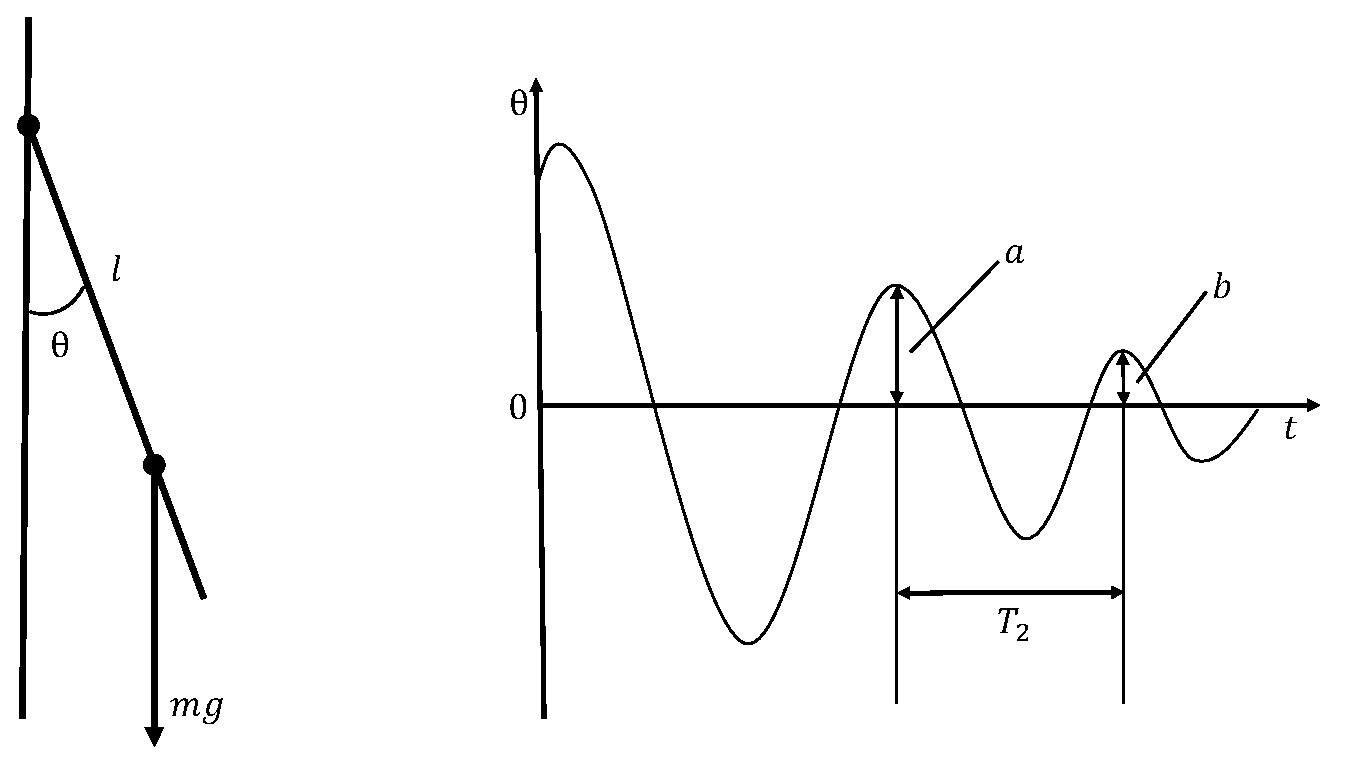
\includegraphics[width=1.0\linewidth]{gazo/ParameterJC.eps}
		\caption{$J$と$c$の測定}
		\label{image:parameterJC}
	\end{figure}
	\par
	いま、減衰振動の周期を$T_{2}$とし、時刻$t_{1}$と時刻$t_{2} = t_{1}+T_{2}$において波形
	$y_{2}(t)$の山が隣合うものとする。このときの振幅の減衰比は
	\[
		\frac{|y_{2}(t_{2})|}{|y_{2}(t_{1})|} = \exp{(-\lambda)}
	\]
	ただし
	\[
		\lambda = \frac{2\pi\zeta}{\omega_{n}\sqrt{1-\zeta^2}}
	\]
	となる。この$\lambda$は対数減衰比と呼ばれる。また
	\[
		T_{2} = \frac{2\pi}{\omega_{n}\sqrt{1-\zeta^{2}}}
	\]
	が成り立つ。したがって、$J$と$c$は
	\[
		J=\frac{mglT_{2}^{2}}{4\pi^{2}+\lambda^{2}}-ml^{2},\ \ 
		c=\frac{2\lambda(J+ml^{2})}{T_{2}}
	\]
	のように与えられる。\cite{Koga:Binpe}
	以下に振子を自由振動させ得られたデータから計算した$J$と$c$を示す。
	\[
		J=2.5\times10^-4[\rm{khm^{2}}]
	\]
	\[
		c=5.4\times10^-5[\rm{kgm^{2}/s}]
	\]
	
\subsection{Mとfの測定}
	
	$M$と$f$の測定方法には二通りがある。
	\subsubsection{ステップ応答による測定法}
		ここでは、台車をアンプ・モータプーリ・ベルト・台車系の等価質量と等価摩擦係数とし、
		台車のステップ応答を測定することで$M$と$f$を決定する。
		ただし、振り子は台車から取り外した状態で測定を行う。
		このときの運動方程式は
		\[
			M\ddot{r} = au - f\dot{r}
		\]
		であり、$u$から$r$までの伝達関数$G$は
		\[
			G(s) = \frac{K}{s(Ts+1)}
		\]
		となる。ただし、
		\begin{equation}
			K = \frac{a}{f},\ \ T=\frac{M}{f}
			\label{eq:kt}
		\end{equation}
		である。初期状態を0とするとき、このシステムのステップ応答は
		\begin{equation}
			r(t) = KU_{0}\left(Te^{\frac{-t}{T}+t-T}\right)
			\label{eq:step}
		\end{equation}
		である。
		\begin{figure}[H]
			\centering
			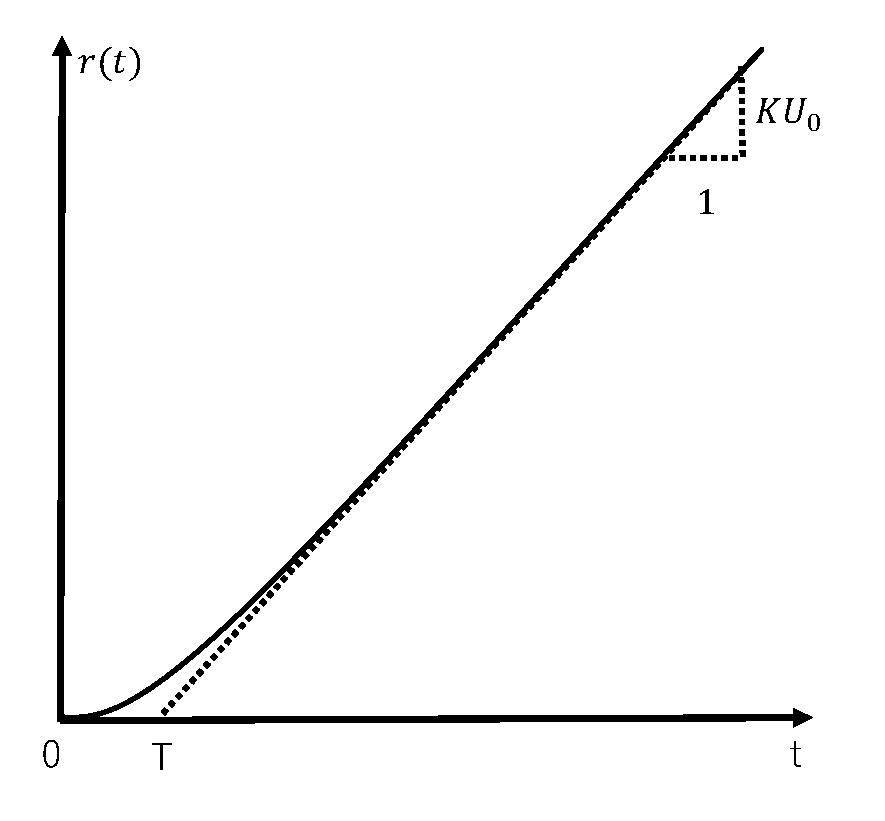
\includegraphics[width=0.6\linewidth]{gazo/step.eps}
			\caption{台車のステップ応答}
			\label{image:parameterMF}
		\end{figure}
		ただし、$U_{0}$はステップの高さである。
		(\ref{eq:step})において$t→\infty$とすれば
		\[
			r(t) = KU_{0}(t-T)
		\]
		となり、図\ref{image:parameterMF}を参考に$T$と$K$をもとめ、
		(\ref{eq:kt})式より$M$と$f$を決定することができる。
		以下にこの方法を用いて同定したパラメータを示す。
		\[
			M=6.9E-1(\rm{kg})
		\]
		\[
			f=7.6(\rm{kg/s})
		\]
		
	\subsubsection{フィードバック入力による測定法}
		ここでは、入力にステップ応答ではなく、以下に示すようなフィードバック入力を加える。
		\begin{equation}
			u = k_{c}(y_{c} - y)
		\end{equation}
		ただし、$y_c$は目標値、$y$は出力、$k_{c}$はフィードバックゲインである。
		本節では$k_c=2500$とする。
		このようにすることで不足制動の2次系($\zeta<1$)を実現させる。
		\begin{figure}[H]
			\centering
			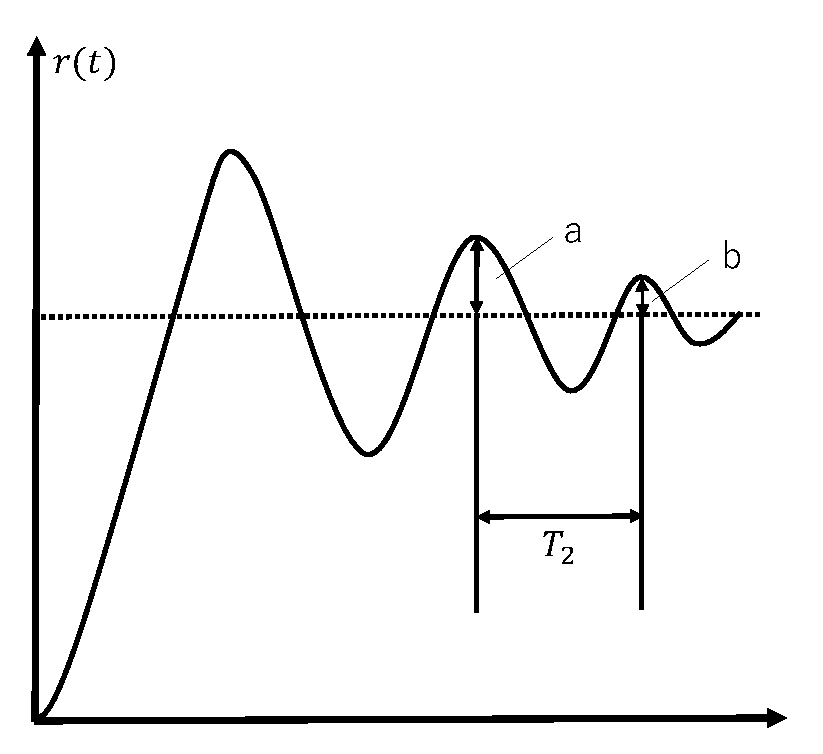
\includegraphics[width=0.6\linewidth]{gazo/feedback.eps}
			\caption{台車のフィードバック応答}
			\label{image:parameterMFfeed}
		\end{figure}
		図\ref{image:parameterMFfeed}を参考にして$M$と$f$を同定する。
		この方法は$J$と$c$の同定の際に用いた方法とほぼ同じであるため、詳しい説明はそちらに
		譲る。
		\par
		台車のフィードバック応答から求めた$\lambda$と$T_2$から以下の式を用いて$\zeta$と$\omega_{n}$を計算し求める。
		\begin{equation}
			\lambda=\frac{2\pi\zeta}{\sqrt{1-\zeta^{2}}}
		\end{equation}
		\begin{equation}
			T_{2}=\frac{2\pi}{\omega_{n}\sqrt{1-\zeta^{2}}}
		\end{equation}
		上の式を式変形して$\zeta$と$\omega_{n}$イコールの式にすると
		\begin{equation}
			\zeta=\frac{\lambda}{\sqrt{4\pi^{2}+\lambda^{2}}}
		\end{equation}
		\begin{equation}
			\omega_{n}=\frac{2\pi}{T_{2}\sqrt{1-\zeta^{2}}}
		\end{equation}
		以上の式から求めた$\zeta$と$\omega_{n}$は以下の二次系の伝達関数の基本形に代入することで
		同定に用いたフィードバック制御系の伝達関数を求めることができる
		\begin{equation}
			G(s) = \frac{\omega_{n}^{2}}{s^{2}+2\zeta\omega_{n}s + \omega_{n}^{2}}
		\end{equation}
		また、今回のフィードバック制御系におけるブロック線図は以下のようになる。
		\begin{figure}[H]
			\centering
			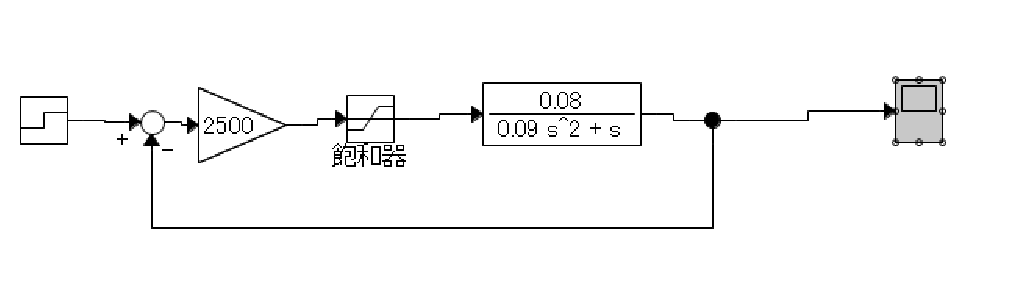
\includegraphics[width=1.0\linewidth]{gazo/FeedBackCart.eps}\\
			\caption{フィードバック制御系のブロック線図}
			\label{image:FeedBackCart}
		\end{figure}
		ここで、$P(s)$は台車の伝達関数であり以下の式で表される。
		\begin{equation}
			P(s)=\frac{K}{s(Ts+1)}
			\label{eq:Ps}
		\end{equation}
		ただし、Tは$M/f$、Kは$a/f$である。上のブロック線図から伝達関数を求める。
		しかし、飽和システムを含んでいると伝達関数を求めることができないので、ここでは飽和システムがなくても
		台車は問題なく動作するものとして仮定する。以上の仮定から伝達関数は
		\begin{equation}
			G(s) = \frac{AK/T}{s^{2}+(1/T)s+(AK/T)}
			\label{eq:Gs}
		\end{equation}
		となる。ただしAはゲインである。(\ref{eq:Ps})式と(\ref{eq:Gs})式を係数比較し、$M,f$イコール
		の式にすると以下のようになる。
		\begin{equation}
			\left.
			\begin{array}{l}
				\displaystyle M=\frac{aA}{\omega_{n}^{2}} \\
				f=2\zeta\omega_{n}^{2}M
			\end{array}
			\right.
			\label{eq:mf}
		\end{equation}
		よって、(\ref{eq:mf})式からMとfは以下のように求まる。
		\[
			M=1.59(\rm{kg})
		\]
		\[
			f=13.2(\rm{kg/s})
		\]
		
	\subsubsection{$M$と$f$の決定}
	パラメータ$M$と$f$についてはステップ応答による方法とフィードバックによる方法の2通りから
	同定を行った。しかし、それぞれの方法で求めたパラメータを比較するとまるで違うことがわかる。
	これはフィードバックによる方法が十分に正確な方法ではなかったためといえる。
	その原因は、飽和システムを含めずに同定を行ったことではないかと考える。
	シミュレーションにおいては入力にどのような値を加えても倒立振子系に何ら影響はないが
	実際の倒立振子においてはその入力できる値には制限がある。この制限を考えるか否か
	で結果が変わってくるはずである。
	\begin{figure}[H]
		\centering
		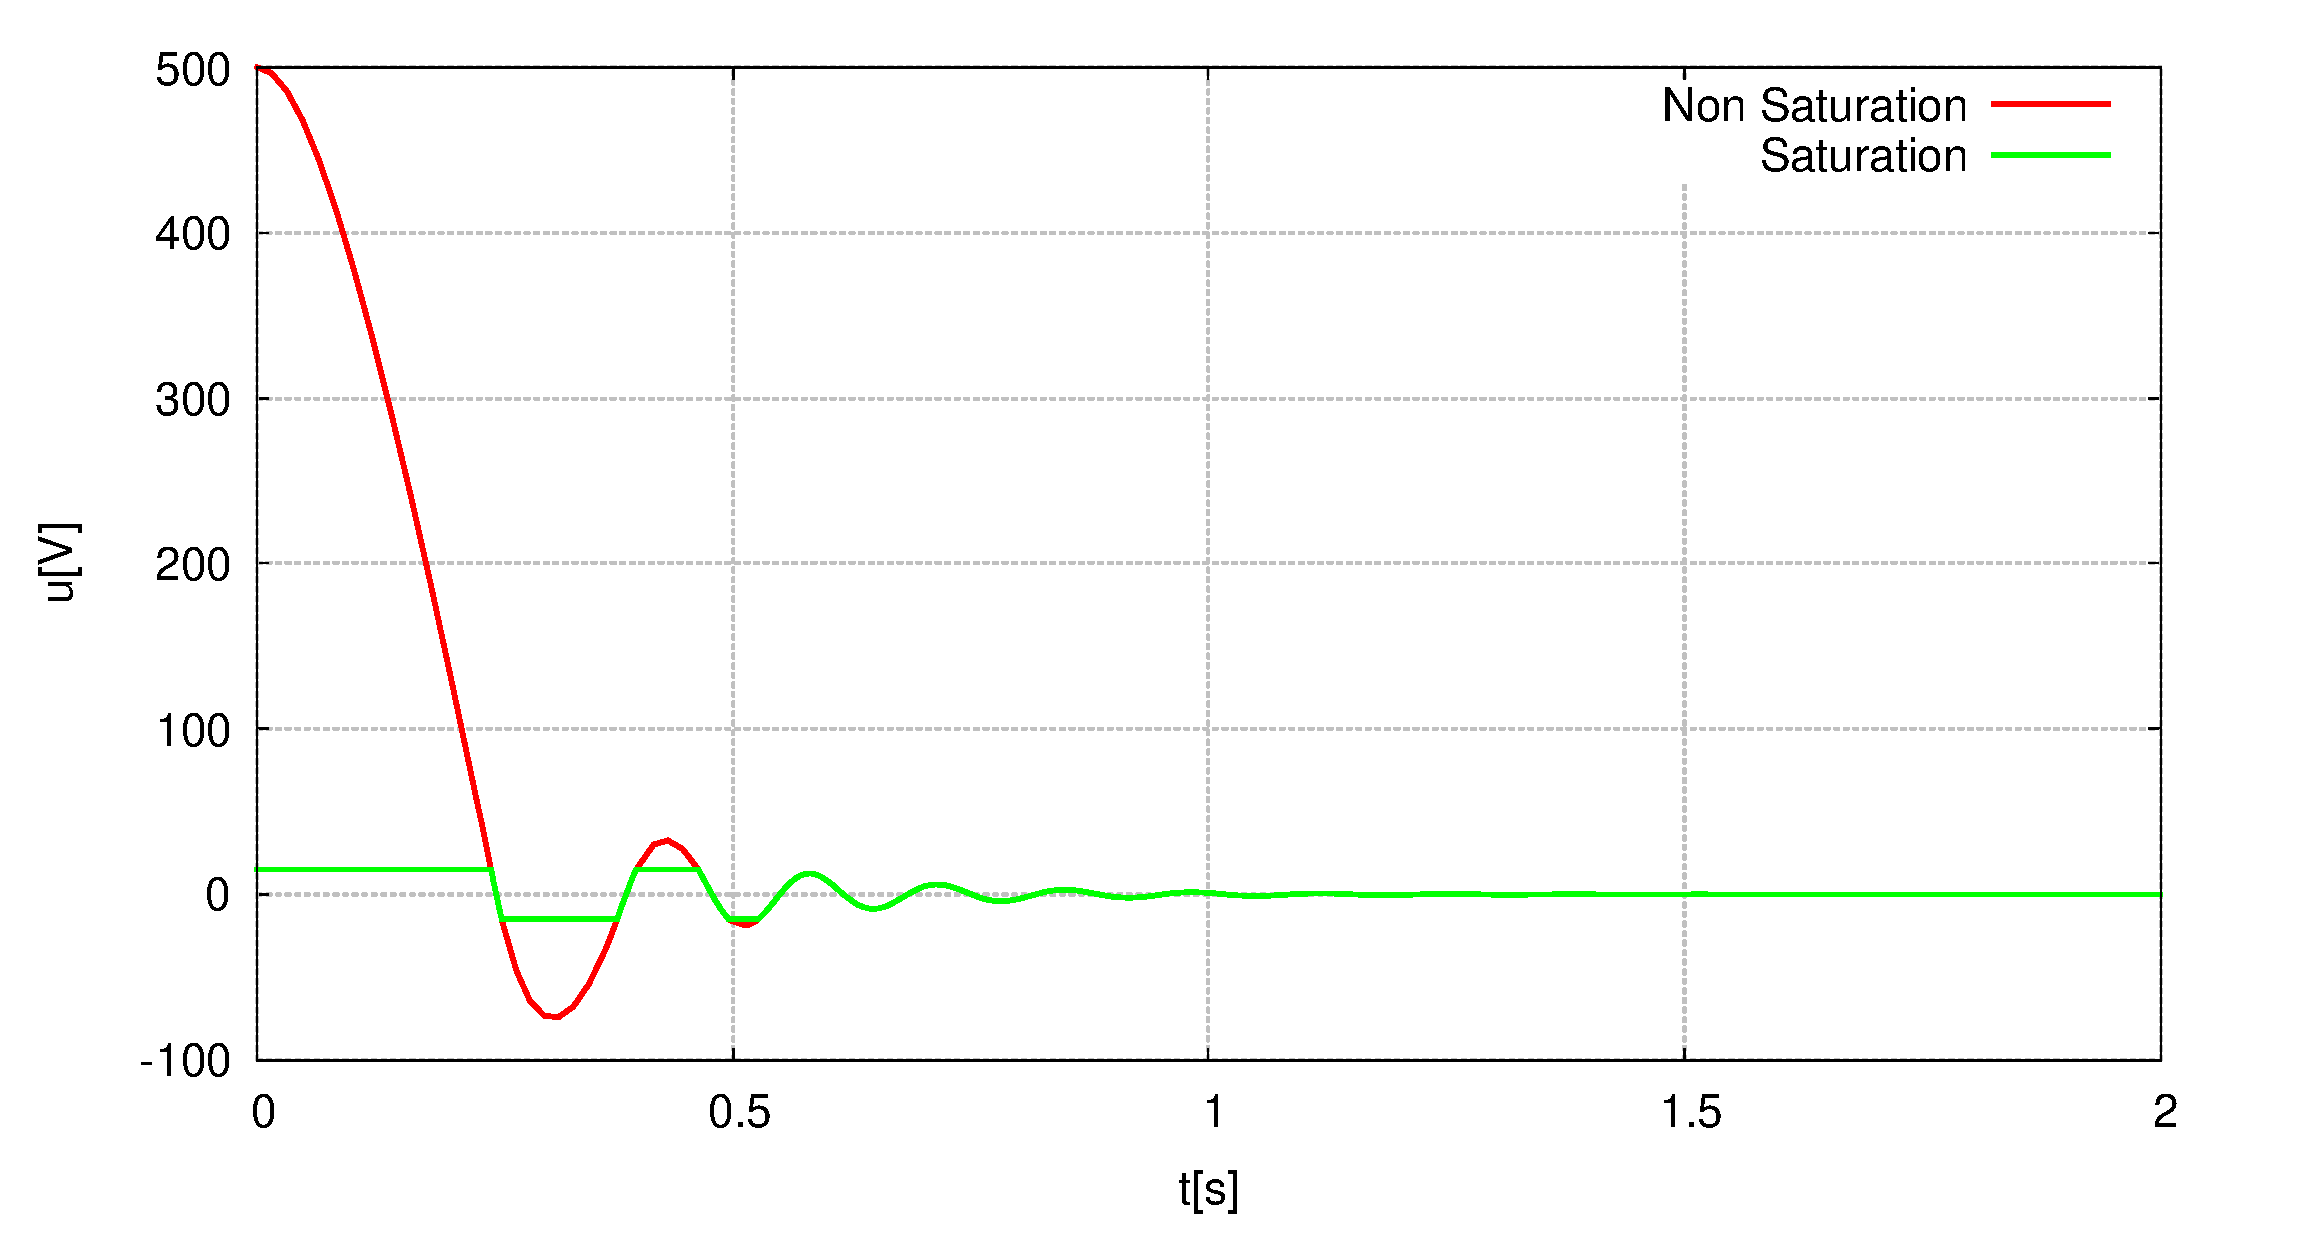
\includegraphics[width=0.8\linewidth]{gazo/feedback_input.eps}\\
		\caption{飽和器の有無によるフィードバック入力の比較}
		\label{image:feedback_saturation}
	\end{figure}
	図\ref{image:feedback_saturation}は図\ref{image:FeedBackCart}のブロック線図において
	飽和器を含めた場合の入力と飽和器を含めなかった場合の入力を描画させたものである。
	この図より、飽和器がない(non Saturation)場合、入力は最大500(V)まで加えられることがわかる。本実験で用いる倒立振子系の入力限界は
	$-15<u<15$であるので、飽和器を加えた場合、その範囲を超える入力は絶対値15(V)に制限されている。
	つまり、フィードバックによる方法で同定したパラメータは飽和器を考慮していないので、現実の倒立振子系とは違うパラメータであるといえる。
	また、今回はフィードバックゲインを2500としたが、
	フィードバックゲインを小さくすると、入力もそれに伴い小さくなるので、
	現実の倒立振子系に近いパラメータを同定することができるはずである。
	以上から本実験においてフィードバックを行う場合、入力が大きく跳ね上がる可能性があるので、必ず飽和システムが必要であるといえる。
	なので、飽和システムが存在する限り伝達関数を求めることができないので、
	正確なパラメータの計算を行うことができないといえる。
	以降、パラメータ$M,f$はステップ応答による方法で同定した値を用いる。
	
\subsection{$c_1$と$c_2$の測定}
	$c_1$と$c_2$に関しては
	\[
		c_1 = 1.0 [\rm{V/m}]
	\]
	\[
		c_2 = 1.0[\rm{V/rad}]
	\]
	というように
	ソフトウェアに設定してあるものを用いた。
\subsection{同定結果}
	同定実験において同定したパラメータを表にまとめる。
	\begin{table}[htb]
		\begin{center}
			\caption{同定したパラメータの一覧}
			\medskip
			
			\begin{tabular}{|l|l|}\hline
				パラメータ & 同定した値 \\ \hline\hline
				m[kg]  & 0.031\\ \hline
				l[m] & 0.15\\ \hline
				M[kg] & 0.69\\ \hline
				f[kg/s] & 7.6\\ \hline
				J[$\rm{kgm}^2$] & $2.5\times10^{-4}$\\ \hline
				c[$\rm{kgm}^2/\rm{s}$] & $5.4\times10^{-5}$\\ \hlinesa
				a[N/V] & 0.61\\ \hline
				$c_{1}$[V/m] & 1.0\\ \hline
				$c_{2}$[V/m] & 1.0\\ \hline
			\end{tabular}
		\end{center}
	\end{table}
%一次チェック完了:
%-----------------------------------------------------------------------------------------------------	
\section{パラメータの検証}
	前節では、実験によって倒立振子のパラメータを同定した。
	しかし、その同定したパラメータがどれほど有効性があるか現時点では全く分からない状況である。
	そこで、本節では同定したパラメータの有効性をがどれほどなのかシミュレーションを用いて検証を
	行う。シミュレーションに用いたツールはJAMOXである。ただし、直接同定を行った$m,l$や最初から
	設定してあった$c_1,c_2$については検証は行わない。
	\subsection{振子の自由振動シミュレーション}
		ここでは、$J,c$の検証を行う。
		以下にシミュレーションと実験データを描画したグラフを示す。
		\begin{figure}[H]
			\centering
			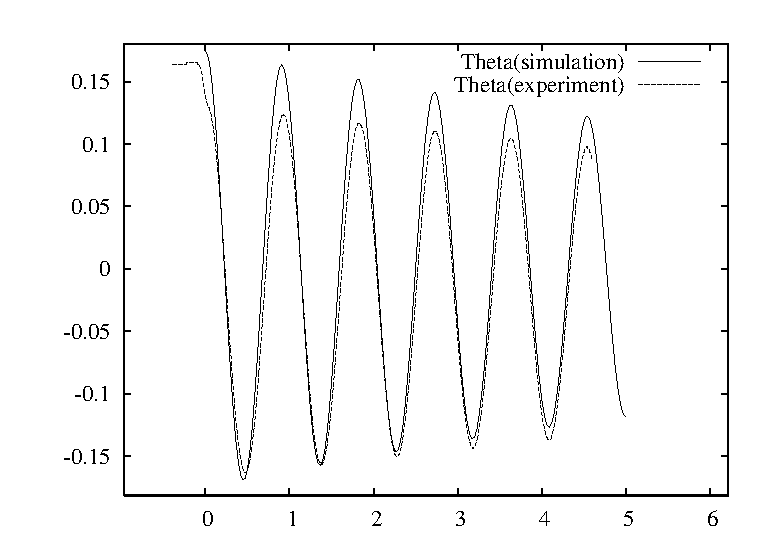
\includegraphics[width=0.8\linewidth]{gazo/free45Auto.eps}\\ 
			\caption{振子の自由振動シミュレーション}
			\label{image:freependulum}
		\end{figure}
		図\ref{image:freependulum}において、シミュレーションは0.32(s)程遅らせて実行しているので、それ以前の時間の角度は$0°$である。
		自由振動の初期角度は$180°$を基準として$10°$である。
		図\ref{image:freependulum}よりシミュレーションと実験結果に少し差異はあるが
		大きな違いはないといえる。よって同定したパラメータ$J,c$は有効な値であるといえる。
		\newpage
	\subsection{台車のステップ応答による方法のシミュレーション}
		ここでは、$M,f,a$の検証を行う。$M,f$はステップ応答による方法で求めた値を用いる。
		以下にシミュレーションと実験データを描画したグラフを示す。
		\begin{figure}[H]
			\centering
			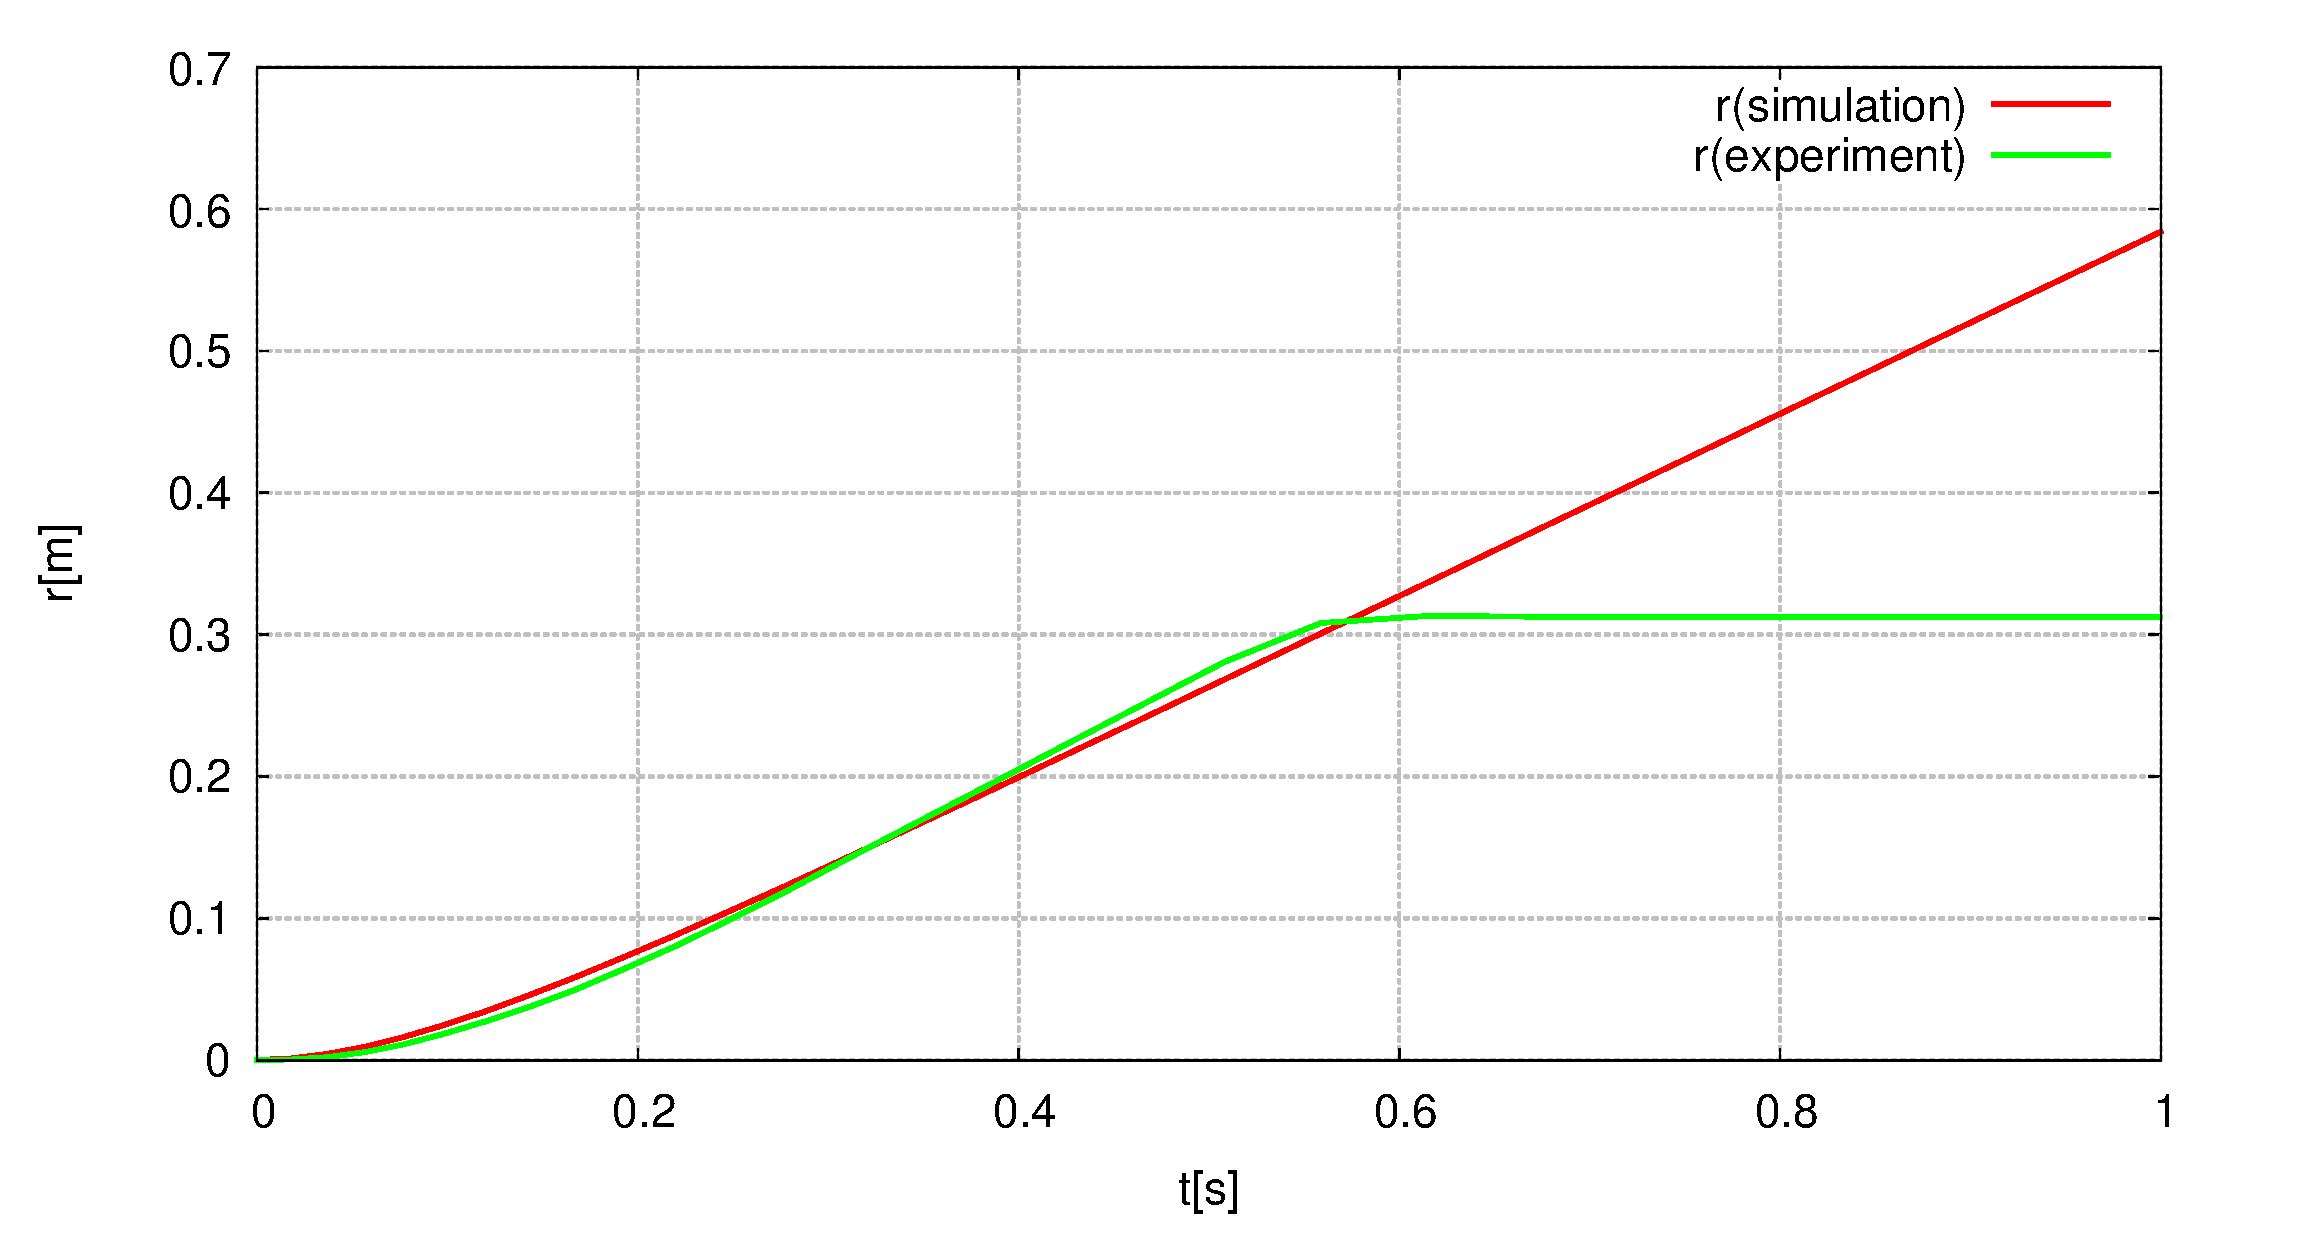
\includegraphics[width=0.8\linewidth]{gazo/nabe8.eps}\\
			\caption{台車のステップ応答シミュレーションと実験結果の比較}
			\label{image:step}
		\end{figure}
		図(\ref{image:step})よりシミュレーションと実験結果に少し差異はあるが
		大きな違いはないといえる。0.6秒以降のグラフが大幅に異なっているが、これはシミュレーションの場合は
		台車の可動範囲に制限がないためずっと台車が移動し続けるが、実験の場合は台車の可動範囲に
		制限があるため、ある時間を境に移動が止まっている。また、このときの入力電圧は$8[\rm{V}]$
		である。以上から同定したパラメータ$M,f,a$は有効な値といえる。
		\newpage
	\subsection{台車のフィードバック応答シミュレーション}
		ここでは、$M,f,a$の検証を行う。$M,f$はフィードバックによる方法で求めた値を用いる。
		%ここの画像はあやしいので差し替え推奨
		以下にシミュレーションと実験データを描画したグラフを示す。ただし、フィードバックゲインは$1500$である。
		\begin{figure}[H]
			\centering
			\includegraphics[width=0.8\linewidth]{gazo/feedbackExperiment.eps}
			\caption{フィードバックによる方法のシミュレーションと実験結果の比較}
			\label{image:feedback}
		\end{figure}
		図\ref{image:feedback}よりシミュレーションと実験結果には大きな差異があることが確認できる。
		上述した通りこの方法で同定したパラメータは現実の倒立振子系に即しておらず、結果実験で得られた波形との
		比較において大きな違いが出てきてしまう。よってこの方法で同定したパラメータ$M,f$には
		有効性がないといえる。
		
\section{設計(線形)モデルの決定}
	ここまでで、パラメータを同定し、その有効性についても確かめた。よって、同定すべきパラメータを決定できたので
	システム行列A、入力行列B、出力行列Cを\MaTX{}を用いて計算し、倒立振子の線形モデルを確定する。
	\MaTX{}で計算した各行列を以下に示す。
	\begin{equation}
		A=\left[
		\begin{array}{cccc}
			0 & 0 & 1 & 0 \\
			0 & 0 & 0 & 1 \\
			0 & -0.32 & -10.9 & 0.00038 \\
			0 & 50 & 53 & -0.059 \\
		\end{array}
		\right]
	\end{equation}
	\begin{equation}
		B=\left[
		\begin{array}{c}
			0 \\
			0 \\
			0.87 \\
			-4.3 \\
		\end{array}
		\right]
	\end{equation}
	\begin{equation}
		C=\left[
		\begin{array}{cccc}
			1 & 0 & 0 & 0 \\
			0 & 1 & 0 & 0 \\
		\end{array}
		\right]
	\end{equation}
	ただし、倒立振子を立たせることを目的とするので、上向きを基準としたときの線形状態方程式である。
	%一次チェック完了:
	%---------------------------------------------------------------
\chapter{制御系設計}  
	\section{システム解析}
	前章で確定した線形モデルについてシステム解析を行う。これにより今回用いるモデルが安定化制御可能か
	判定することができる。具体的には可制御性と可観測性を調べ、それらが存在すれば安定化制御可能であるといえる。
	以下で行う計算はすべて\MaTX{}を用いた。
	\subsection{安定性}
		システムの極(Aの固有値)を計算した結果$D$を以下に示す。
		\begin{equation}
			D=\left[
			\begin{array}{c}
				7.0+0i\\
				0+0i \\
				-6.8-0i \\
				-11+0i\\
			\end{array}
			\right]
			\label{eq:Aeig}
		\end{equation}
		(\ref{eq:Aeig})式より1行目が不安定であり、2行目が安定限界であるので、今回用いるモデルは
		不安定であるといえる。
	\subsection{可制御性}
		可制御性行列は以下のようになる。
		\begin{equation}
			N_{c} = \left[
			\begin{array}{cccc}
				C & CA & CA^{2} & CA^{3} \\
			\end{array}
			\right]
		\end{equation}
		上の行列よりランクは4になれば可制御性があるといえる。ランクを計算したところ
		\begin{equation}
			rank  = 4
		\end{equation}
		となった。よって可制御性を確認できる。\\
	\subsection{可制御性}
		可観測性行列は以下のようになる。
		\begin{equation}
			N_{o} = \left[
			\begin{array}{c}
				C\\
				CA\\
				CA^{2}\\
				CA^{3}\\
			\end{array}
			\right]
		\end{equation}
		上の行列よりランクは4になれば可観測性があるといえる。ランクを計算したところ
		\begin{equation}
			rank = 4
		\end{equation}
		となった。よって、可観測性を確認できる。\\
	\par
	以上から倒立振子系の上向き基準の線形モデルは不安定なシステムであるが、4つの状態を観測することができ、
	制御することが可能なシステムといえる。次の節では倒立振子を立たせるための制御器を設計していく。
	その際にここで計算したシステム行列Aと入力行列Bを用いる。
		
%----------------------------------------------------------------------------------
\section{状態フィードバックの設計}
	制御器を設計していく第一段階として、状態フィードバック$F$の設計を行う。
	$F$は、システムを安定化する状態フィードバック
	\[
		u = -Fx
	\]
	として求めればよい。
	また、本実験においては台車が目標値へ移動を行う場合があるので、目標値$x_{ref}$
	として以下を設計することになる。
	\begin{equation}
		u(t) = F(x_{ref} - x)
		\label{eq:Feq1}
	\end{equation}
	% TODO
	この状態フィードバックの設計法には、極配置に基づく状態フィードバック測と
	LQ最適制御に基づく状態フィードバック測の2通りがあるが今回は後者の方法を用いて設計を行う。
	\par
	さて、(\ref{eq:Feq1})式をLQ問題の解として得るために、2次形式評価関数
	\begin{equation}
		J = \int_{0}^{\infty}(x^{T}Qx+Ru^{2})dt
		\label{eq:Feq2}
	\end{equation}
	\begin{equation}
		Q = diag(q_{1}^2,q_{2}^2,q_{3}^2,q_{4}^2),\ \ R = 1
		\label{eq:Feq3}
	\end{equation}
	を考える。ただし、 $diag(\ldots)$は、対角行列を表す。これは
	\begin{equation}
		J=\int_{0}^{\infty}(q_{1}^{2}r^{2}+q_{2}^{2}\theta^{2}
		+q_{3}^{2}\dot{r}^{2}+q_{4}^{2}\dot{\theta}^{2})dt
	\end{equation}
	のように表されることから、$q_1,q_2,q_3,q_4$は台車位置$r$、振り子角度$\theta$、
	台車速度$\dot{\theta}$、振子角速度$\dot{\theta}$の間のバランスをとる重み係数である。
	\par
	(\ref{eq:Feq2})、(\ref{eq:Feq3})式を最小にする(\ref{eq:Feq1})式における$F$は、
	リカッチの方程式
	\[
		A^{T}P+PA-PBR^{-1}B^{T}P+Q = 0
	\]
	の解$P>0$を求めて
	\[
		F = R^{-1}B^{T}P
	\]
	のように与えられる。

%----------------------------------------------------------------------------------
\section{最小次元オブザーバの設計}
	第二段階として、状態を推定する状態観測器(最小次元オブザーバ)
	\begin{equation}
		
	\end{equation}

%----------------------------------------------------------------------------------
\section{コントローラの離散化}

%----------------------------------------------------------------------------------
\section{振り上げ制御及び安定化の実現}

%---------------------------------------------------------------------------------- 
\chapter{シミュレーション}
	目標値変更のシミュレーションによって制御器に関する各パラメータの有効な値を探索する。 シミュレーションにはJAMOXを用いた。
% --------------------------------------------------------------------------------------
\section{重み行列の変更による制御性能評価}
	LQ最適制御に基づく状態フィードバック$F$を設計するために
	連続時間線形二次レギュレーターを用いる。この時、連続時間線形二次レギュレーターには
	システム行列$A$と入力行列$B$と重み行列$Q,R$が必要である。
	重み行列は、(\ref{eq:Feq1})式で与え、この重み行列を
	調整することで倒立振子の安定化制御の性能を高めることができる。
	そこで、シミュレーションを用いて重み行列を変更させたときの制御性能について考察していく。
	\par
	今回は行列$R$の値は変更しないので、行列$Q$のみ値を変更してシミュレーション結果を考察する。
	便宜上、重み行列$Q$の対角成分を左から第1成分、第2成分、第3成分、第4成分と呼ぶことにする。
	以下にシミュレーションを行う異なるパターンのパラメータをまとめた表とその時のシミュレーション結果を示す。
	\begin{table}[htb]
		\begin{center}
			\caption{重み行列の変更パターン}
			%\medskip
			\begin{tabular}{|c|c|c|c|}\hline
				& 重み行列$Q$ & オブザーバの極$P$ & サンプリング周期$\Delta[\rm{s}]$ \\ \hline\hline
				パターン1 & $Q_1$:$\rm{diag}(1E5,1E5,1,1)$ & $P_1$:$((-60,0),(-60,0))^{'}$ & $\Delta_1$:0.005 \\ \hline
				パターン2 & $Q_2$:$\rm{diag}(1E6,1E5,1,1)$ & $P_2$:$((-60,0),(-60,0))^{'}$ & $\Delta_2$:0.005 \\ \hline
				パターン3 & $Q_3$:$\rm{diag}(1E5,1E6,1,1)$ & $P_3$:$((-60,0),(-60,0))^{'}$ & $\Delta_3$:0.005 \\ \hline
			\end{tabular}
		\end{center}
		\label{table:QRF}
	\end{table}
	
	\begin{figure}[H]
		\centering
		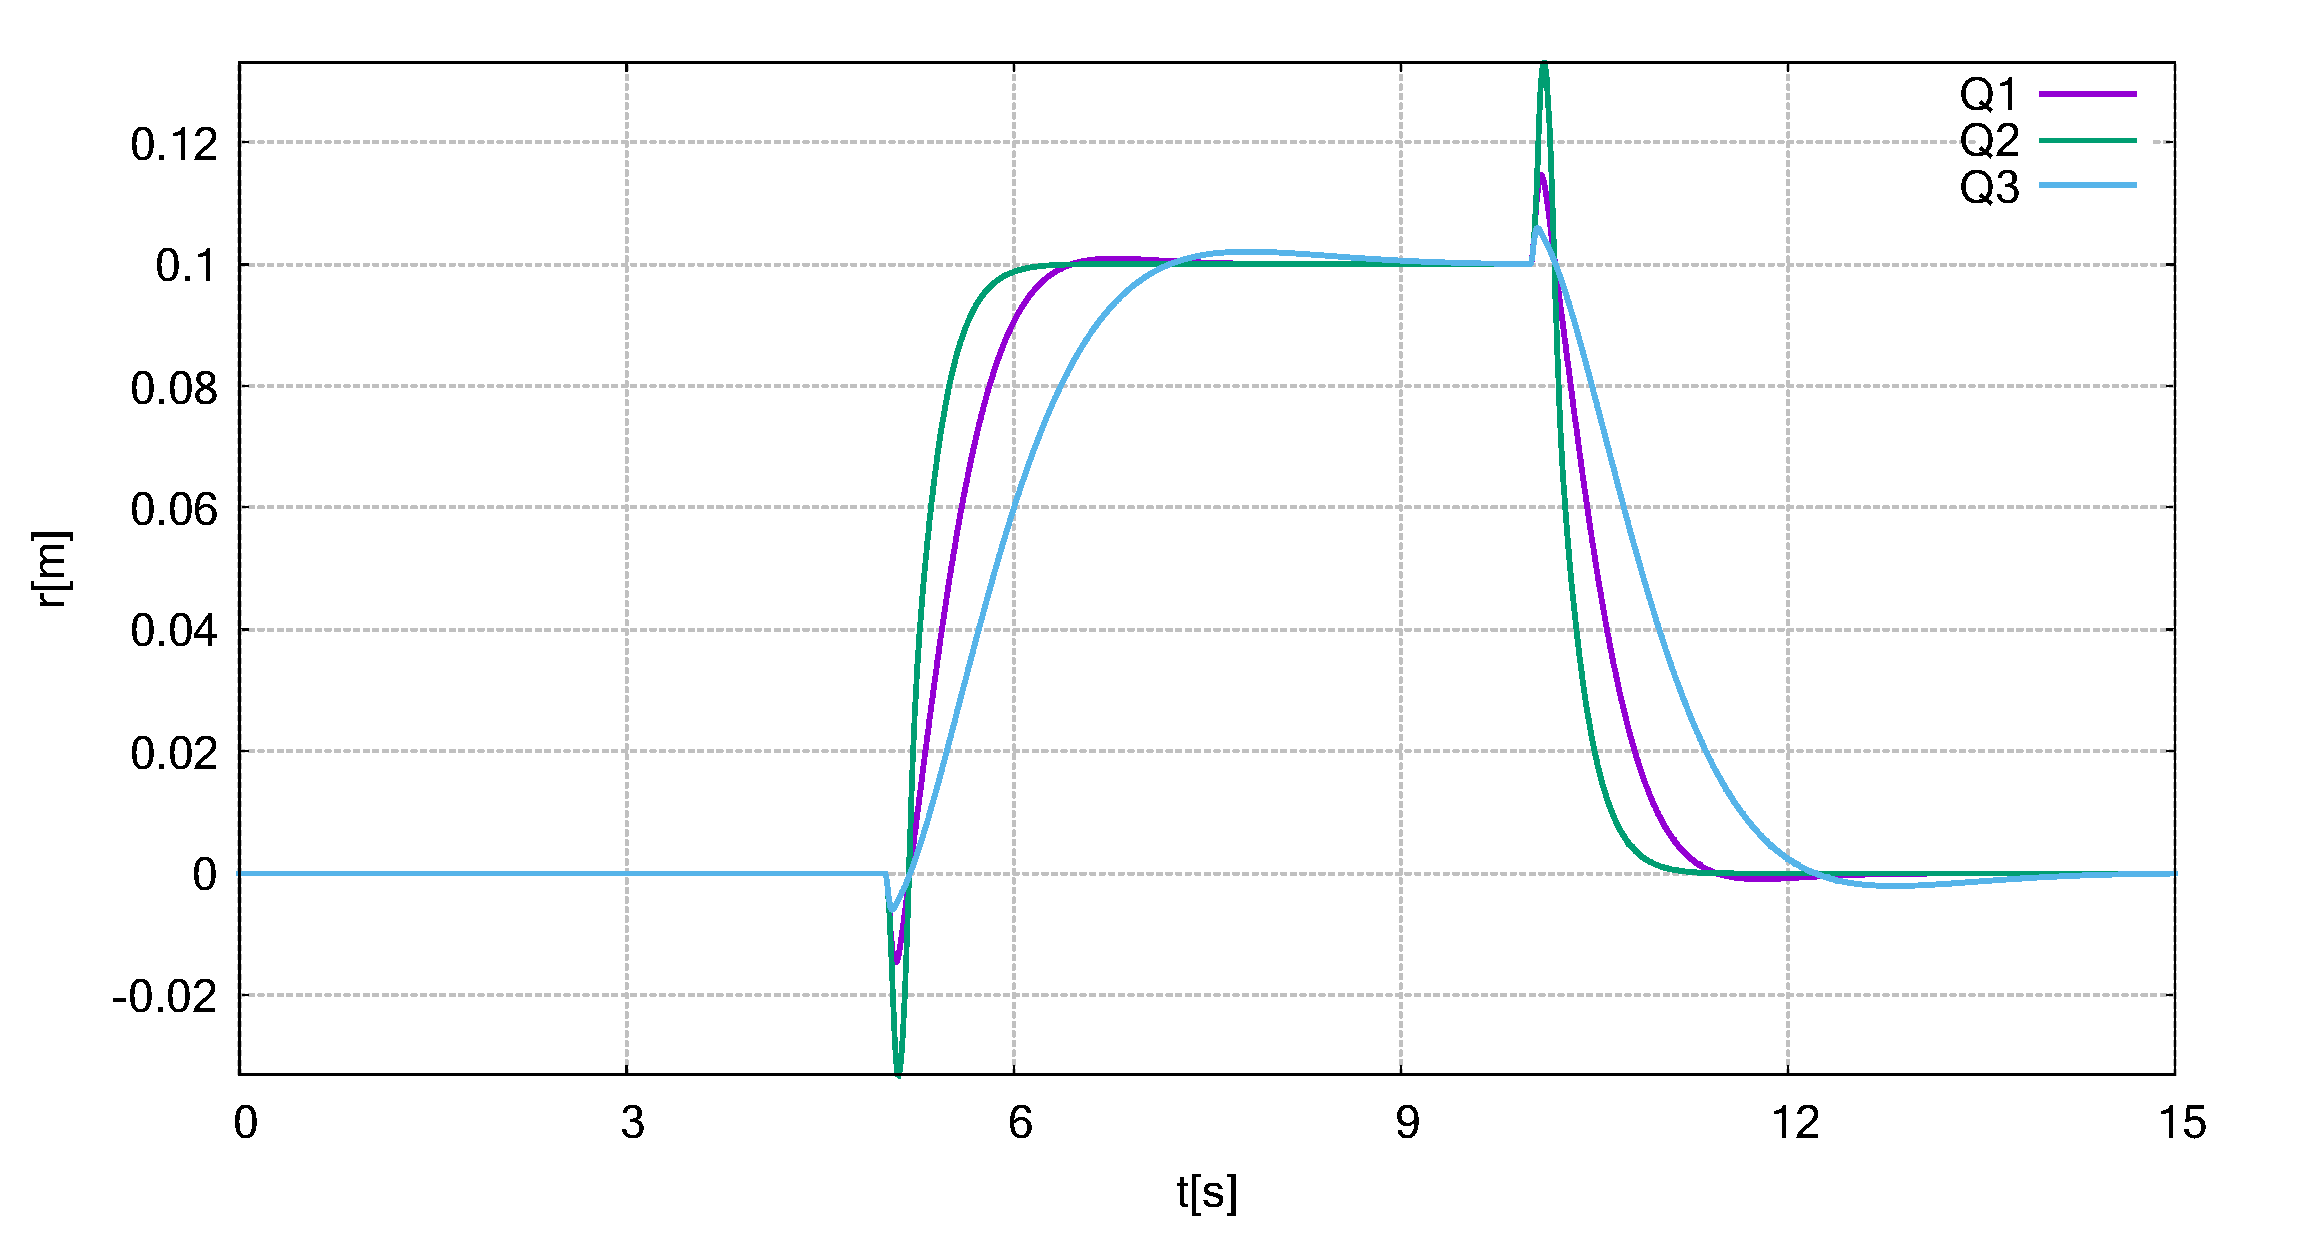
\includegraphics[width=0.8\linewidth]{gazo/simulation_QRF_compare_R.eps}
		\caption{重み行列での比較結果(台車位置)}
		\label{image:simulation_QRF_r}
	\end{figure}
	\begin{figure}[H]
		\centering
		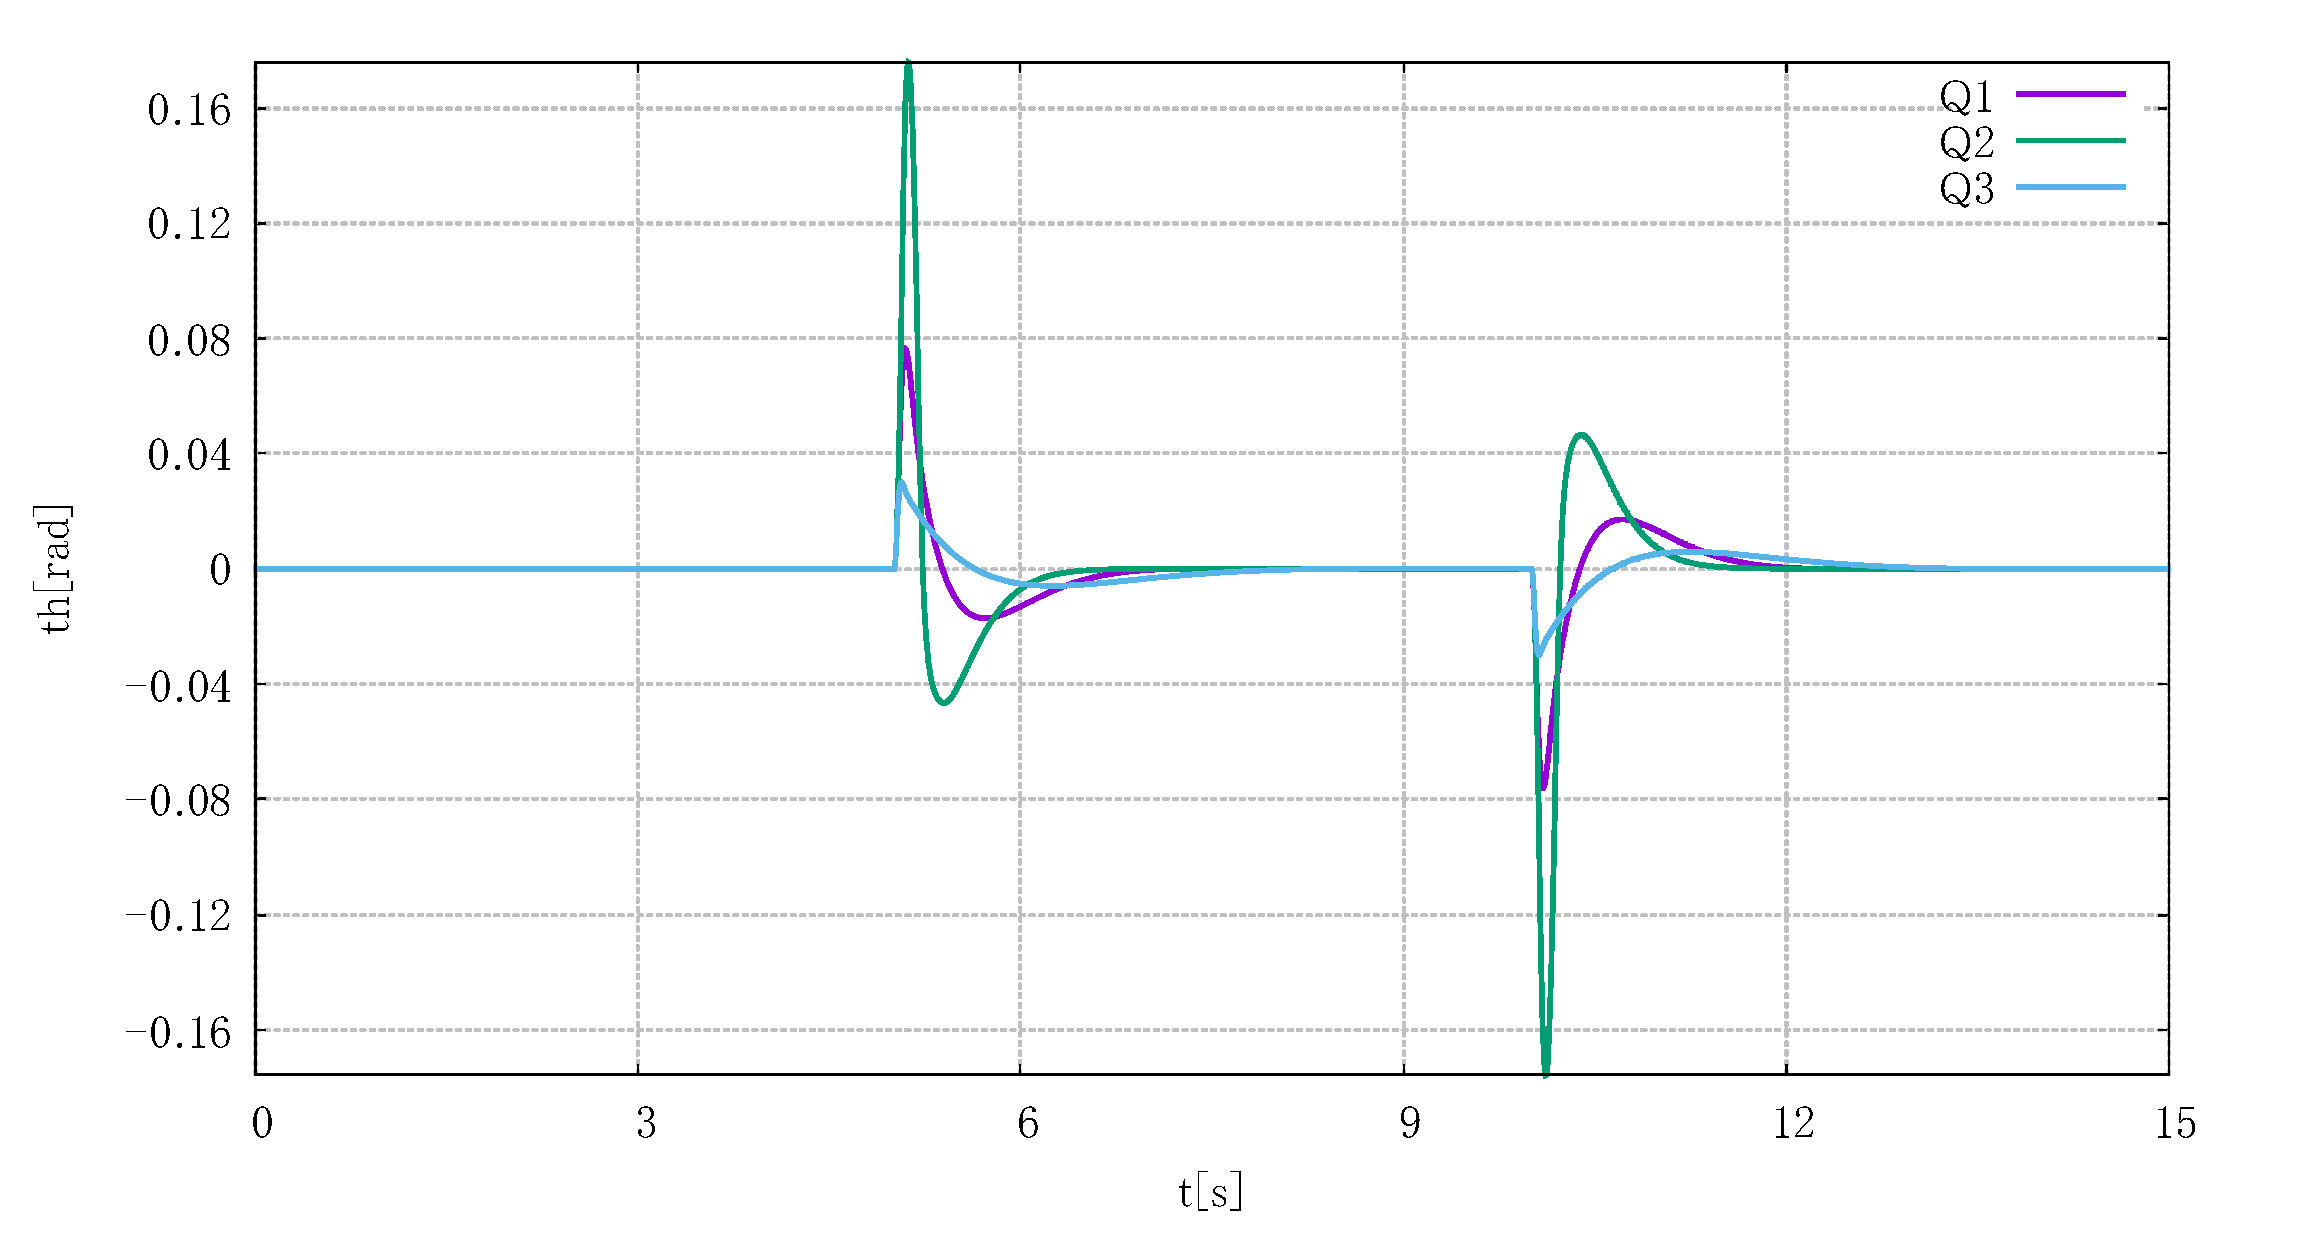
\includegraphics[width=0.8\linewidth]{gazo/simulation_QRF_compare_THETA.eps}
		\caption{重み行列での比較結果(振子角度)}
		\label{image:simulation_QRF_th}
	\end{figure}
	図(\ref{image:simulation_QRF_r})より$Q_2$の応答が一番早く、$Q_3$の応答が一番遅いことが確認できる。このことから台車の位置$r$の応答をよくするには
	重み行列$Q$の第1成分を大きくすればよいとわかる。また、$Q_1$と$Q_3$の第1成分は同じであるのにもかかわらず、$Q_1$の方が応答が早いことが確認できる。これは
	振子の角度$\theta$の応答をよくする第2成分を大きくした分、バランスが第2成分のほうに偏ってしまい、台車の位置の応答が悪くなったといえる。
	\par
	図(\ref{image:simulation_QRF_th})より、振子の角度についても同じことが言え、第2成分を大きくしている$Q_3$の応答が一番よく、$Q_2$の応答が一番悪い結果となっている。
	\par
	以上から重み行列の調整については以下のことが言える。
	\begin{itemize}
	  \item 重み行列$Q$の各成分は$r,\theta,\dot{r},\dot{\theta}$に対応している
	  \item 応答をよくしたい状態があれば、その状態に対応する成分の値を大きくすればよい
	  \item その場合、大きくした成分に対応する状態にバランスが偏る(つまり、ほかの状態の応答が悪くなる)
	\end{itemize}
	
	
% --------------------------------------------------------------------------------------
\section{オブザーバの極の変更による制御性能評価}
	前章で述べたように、最小次元オブザーバを設計するためにゴピナスの方法を用いる。
	この時、システム行列$A$、入力行列$B$、出力行列$C$、オブザーバの極$P$が必要である。
	オブザーバの極$P$を調整することで倒立振子の安定化制御の性能を高めることができる。
	同様にシミュレーションによって制御性能を考察していく。
	\par
	1つ考慮しなければならないのは、オブザーバの極と
	閉ループ系の極(つまり、$(A-BF)$の固有値)との位置関係である。
	閉ループ系の極のうち虚軸に最も近い極を$\lambda_{max}$としたとき、オブザーバーの極$P$は
	\[
		\rm{Re}(P) <5\rm{Re}(\lambda_{max})
	\]
	を満たす考慮して設定する必要がある。
	表(\ref{table:QRF})の$Q_2$を用いて設計した状態フィードバック$F$における閉ループ系の極は
	\begin{equation}
		D=\left[
		\begin{array}{c}
			-0.08\\
			-6.3+1.3i\\
			-6.3+1.3i\\
			-13\\
		\end{array}
		\right]
		\label{eq:Aeig}
	\end{equation}
	である。この中で一番虚軸に近い極は$-0.08$である。よって、少なくともオブザーバーの極$P$は$-0.4$
	より小さい値をとればよいとわかる。
	\par
	以下にシミュレーションを行う異なるパターンのパラメータをまとめた表とその時のシミュレーション結果を示す。
	\begin{table}[htb]
		\begin{center}
			\caption{オブザーバの極の変更パターン}
			\medskip
			
			\begin{tabular}{|c|c|c|c|}\hline
				\ \ & 重み行列$Q$ & オブザーバの極$P$ & サンプリング周期$\Delta[\rm{s}]$ \\ \hline\hline
				パターン1 & $Q_1$:$\rm{diag}(1E5,1E5,1,1)$ & $P_1$:$((-100,0),(-100,0))^{'}$ & $\Delta_1$:0.005 \\ \hline
				パターン2 & $Q_2$:$\rm{diag}(1E5,1E5,1,1)$ & $P_2$:$((-20,0),(-20,0))^{'}$ & $\Delta_2$:0.005 \\ \hline
			\end{tabular}
		\end{center}
		\label{table:QRF}
	\end{table}
	%TODO : シミュレーションを行い図を張り付ける。そのあと考察を述べる
	
	
%--------------------------------------------------------------------------------------
\section{サンプリング周期の変更による制御性能評価}
	離散化を行うサンプリング周期$\Delta$を調整することで倒立振子の安定化制御の性能を高めることができる。
	同様にシミュレーションによって制御性能を考察していく。
	ただし、サンプリング周期が短すぎると実験で用いる倒立振子系においてシステム全体がハングアップする恐れ
	があるため、そのような値においてはシミュレーションを行わない。
	\par
	以下にシミュレーションを行う異なるパターンのパラメータをまとめた表とその時のシミュレーション結果を示す。
	\begin{table}[htb]
		\begin{center}
			\caption{サンプリング周期の変更パターン}
			\medskip
			
			\begin{tabular}{|c|c|c|c|}\hline
				\ \ & 重み行列$Q$ & オブザーバの極$P$ & サンプリング周期$\Delta[\rm{s}]$ \\ \hline\hline
				パターン1 & $Q_1$:$\rm{diag}(1E5,1E5,1,1)$ & $P_1$:$((-20,0),(-20,0))^{'}$ & $\Delta_1$:0.005 \\ \hline
				パターン2 & $Q_2$:$\rm{diag}(1E5,1E5,1,1)$ & $P_2$:$((-20,0),(-20,0))^{'}$ & $\Delta_2$:0.01 \\ \hline
			\end{tabular}
		\end{center}
		\label{table:QRF}
	\end{table}
	%TODO : シミュレーションを行い図を張り付ける。そのあと考察を述べる
%--------------------------------------------------------------------------------------
\section{振り上げ制御及び安定化に対する制御性能評価}
	前節までにおいて、安定化制御における有効なパラメータを考察してきた。
	ここでは、振り上げ制御におけるパラメータ$k,n$を調整することで振り上げ制御の制御性能を考察する。
	\par
	この時、使用した制御器のパラメータの組は以下の表の通りである。
	\begin{table}[htb]
		\begin{center}
			\caption{振り上げ後の安定化制御の際に用いるパラメータの組}
			\medskip
			
			\begin{tabular}{|c|c|c|c|}\hline
				重み行列$Q$ & オブザーバの極$P$ & サンプリング周期$\Delta[\rm{s}]$ \\ \hline\hline
				$Q_1$:$\rm{diag}(1E5,1E5,1,1)$ & $P_1$:$((-20,0),(-20,0))^{'}$ & $\Delta_1$:0.005 \\ \hline
			\end{tabular}
		\end{center}
		\label{table:QRF}
	\end{table}
	
	\begin{table}[htb]
		\begin{center}
			\caption{重み行列の変更}
			\medskip
			
			\begin{tabular}{|c|c|c|c|}\hline
				\ \ & $n$ & $k$ \\ \hline\hline
				パターン1 & $todo$ & $todo$  \\ \hline
				パターン2 & $todo$ & $doto$  \\ \hline
				パターン3 & $todo$ & $doto$  \\ \hline
			\end{tabular}
		\end{center}
		\label{table:QRF}
	\end{table}
	
	
%--------------------------------------------------------------------------------------
\chapter{実験}
	\section{安定化制御実験}
	振子を上向きに配置したときに安定化制御が可能か実験を行う(実験目的の第一項目)。
	その際に、振子を真上に配置するのではなく、十数度角度をつけてから実験を始める。
	実験に用いたパラメータを以下の表に示す。
	\begin{table}[H]
		\begin{center}
			\caption{安定化制御実験で使用したパラメータの組}
			\medskip
			
			\begin{tabular}{|c|c|c|c|}\hline
				重み行列$Q$ & オブザーバの極$P$ & サンプリング周期$\Delta[\rm{s}]$ \\ \hline\hline
				$Q_1$:$\rm{diag}(1E5,1E5,1,1)$ & $P_1$:$((-30,0),(-30,0))^{'}$ & $\Delta_1$:0.005 \\ \hline
			\end{tabular}
		\end{center}
		\label{table:huriage_control}
	\end{table}
	以下に実験結果とシミュレーション結果の比較した図を示す。
	\begin{figure}[H]
		\centering
		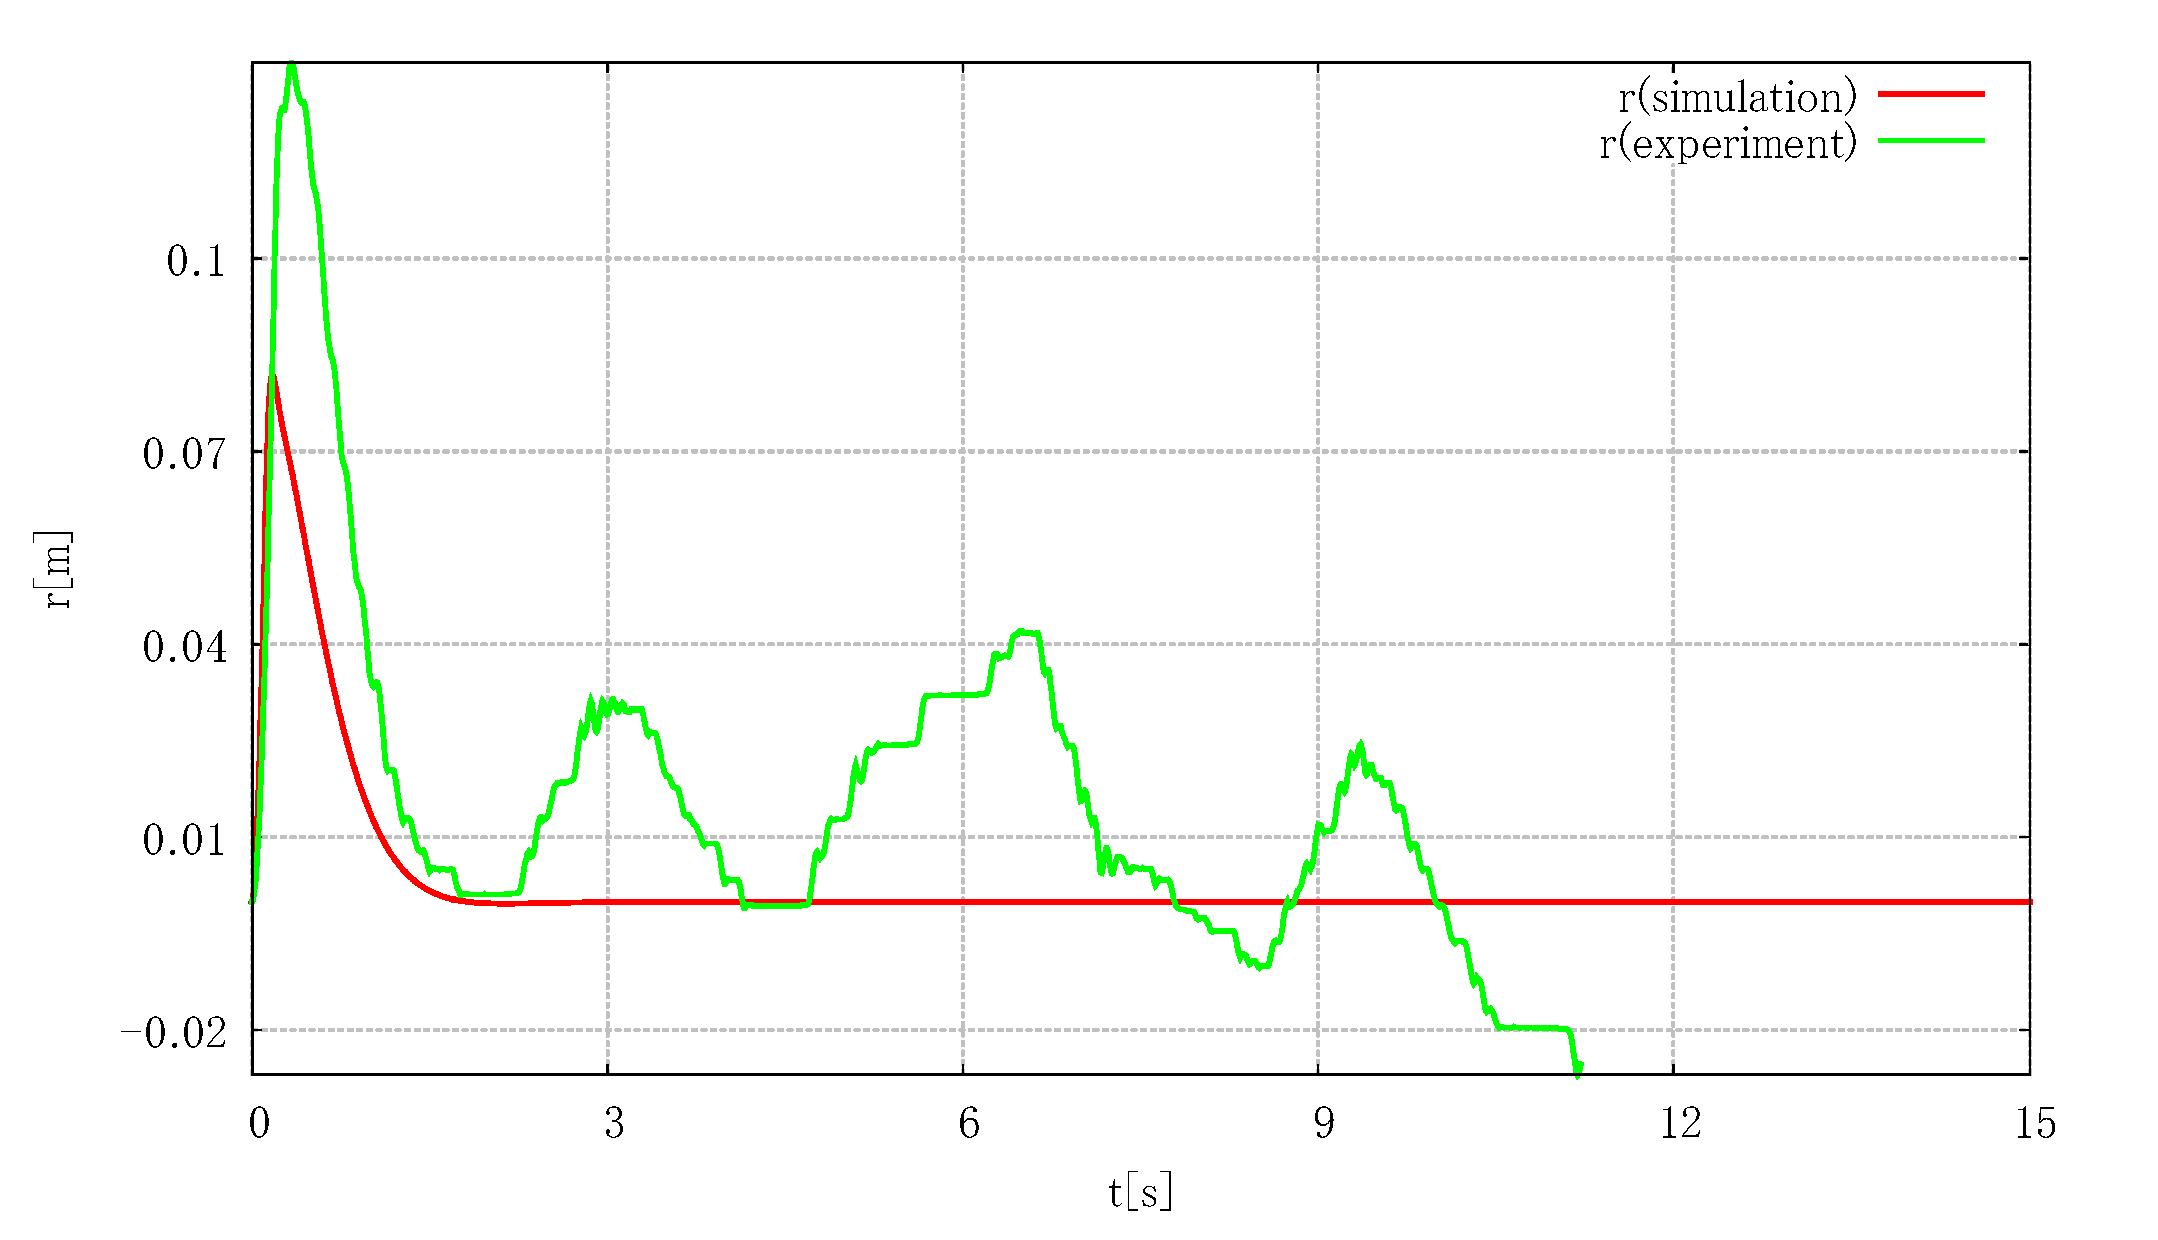
\includegraphics[width=0.8\linewidth]{gazo/experiment_control_R.eps}
		\caption{安定化制御実験結果(台車位置)}
		\label{image:experiment_control_R}
	\end{figure}
	\begin{figure}[H]
		\centering
		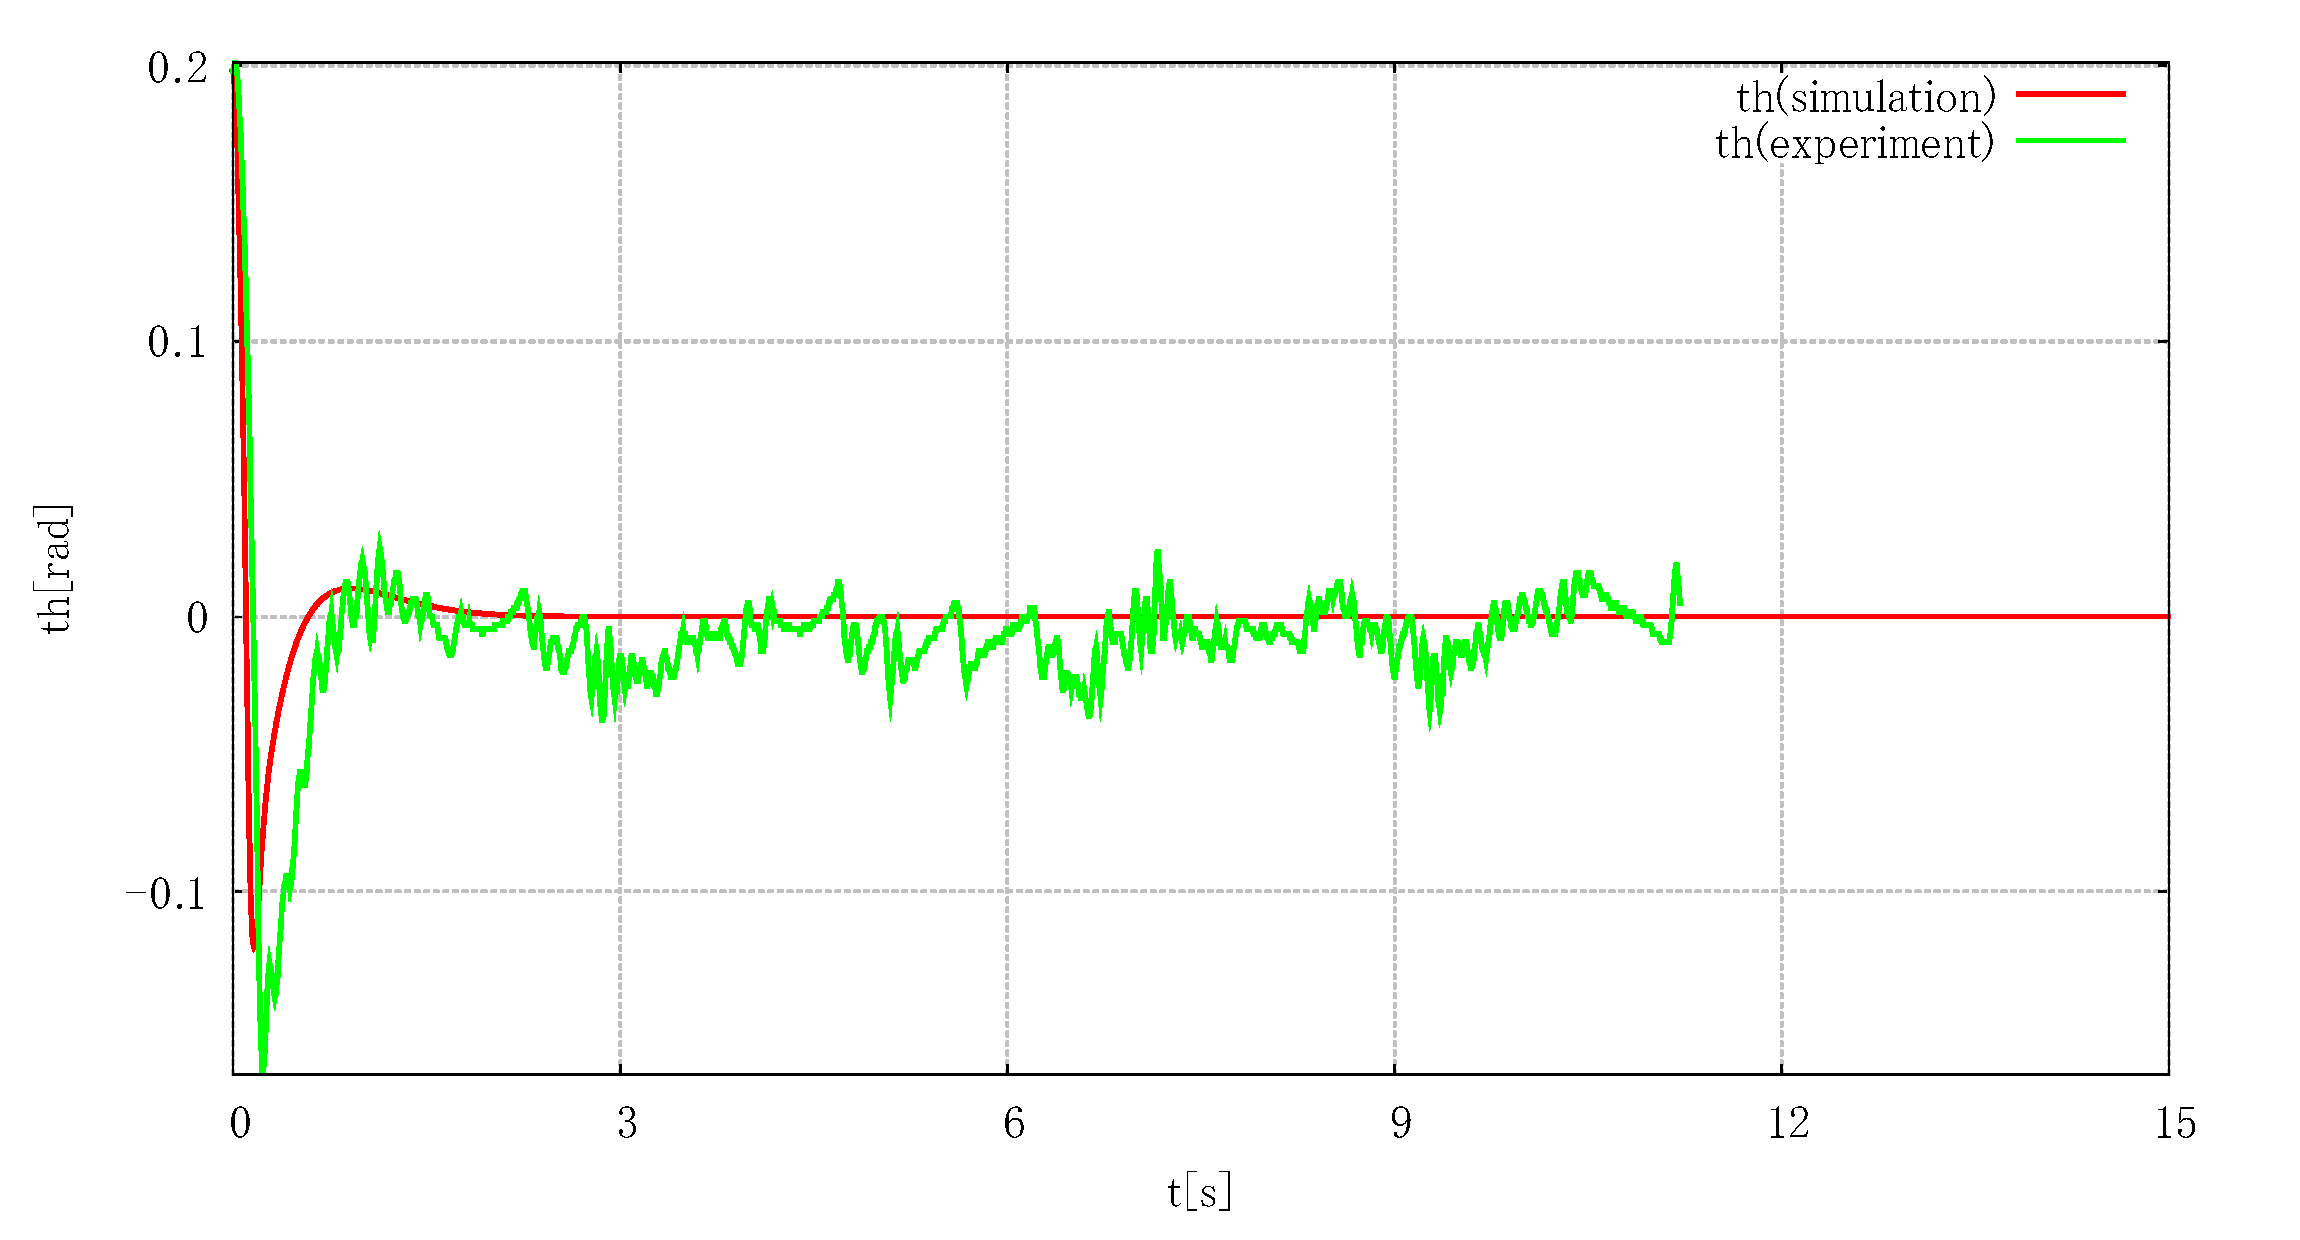
\includegraphics[width=0.8\linewidth]{gazo/experiment_control_TH.eps}
		\caption{安定化制御実験結果(振子角度)}
		\label{image:experiment_control_TH}
	\end{figure}
	図\ref{image:experiment_control_R}と図\ref{image:experiment_control_TH}
	より一番最初の山は実験のほうが大幅に大きくなっていることと、ノイズが乗っている点を除いてシミュレーションと実験結果は
	概ね一致しているといえる。これは、実験のほうではデータの計測を開始して振子から手を離したためその影響が出たといえる。
	この時の初期角度は$11.34°$である。
	よって、初期角度が十数度ある中で実験を開始し、安定化制御を行うことができたため、
	実験目的の第一項目を達成できたといえる。
	
	
	
%-----------------------------------------------------------
\newpage
\section{目標値の変更実験}
	台車に目標値を与えて、その目標値に台車が移動しても安定化制御可能か実験を行う(実験項目の第二項目)。
	なお、目標値は5秒ごとに0→0.1→0のように変更される。
	以下に、重み行列を変更した場合の比較、オブザーバの極を変更した場合の比較、サンプリング周期を変更した場合の比較を
	行った図を示す。
	\par
	%-----------------------------------------------------------------------------------
	\subsection{重み行列の違いによる実験結果の比較}
	最初に重み行列を変更した場合の実験結果の比較を見てみる。
	\begin{figure}[H]
		\centering
		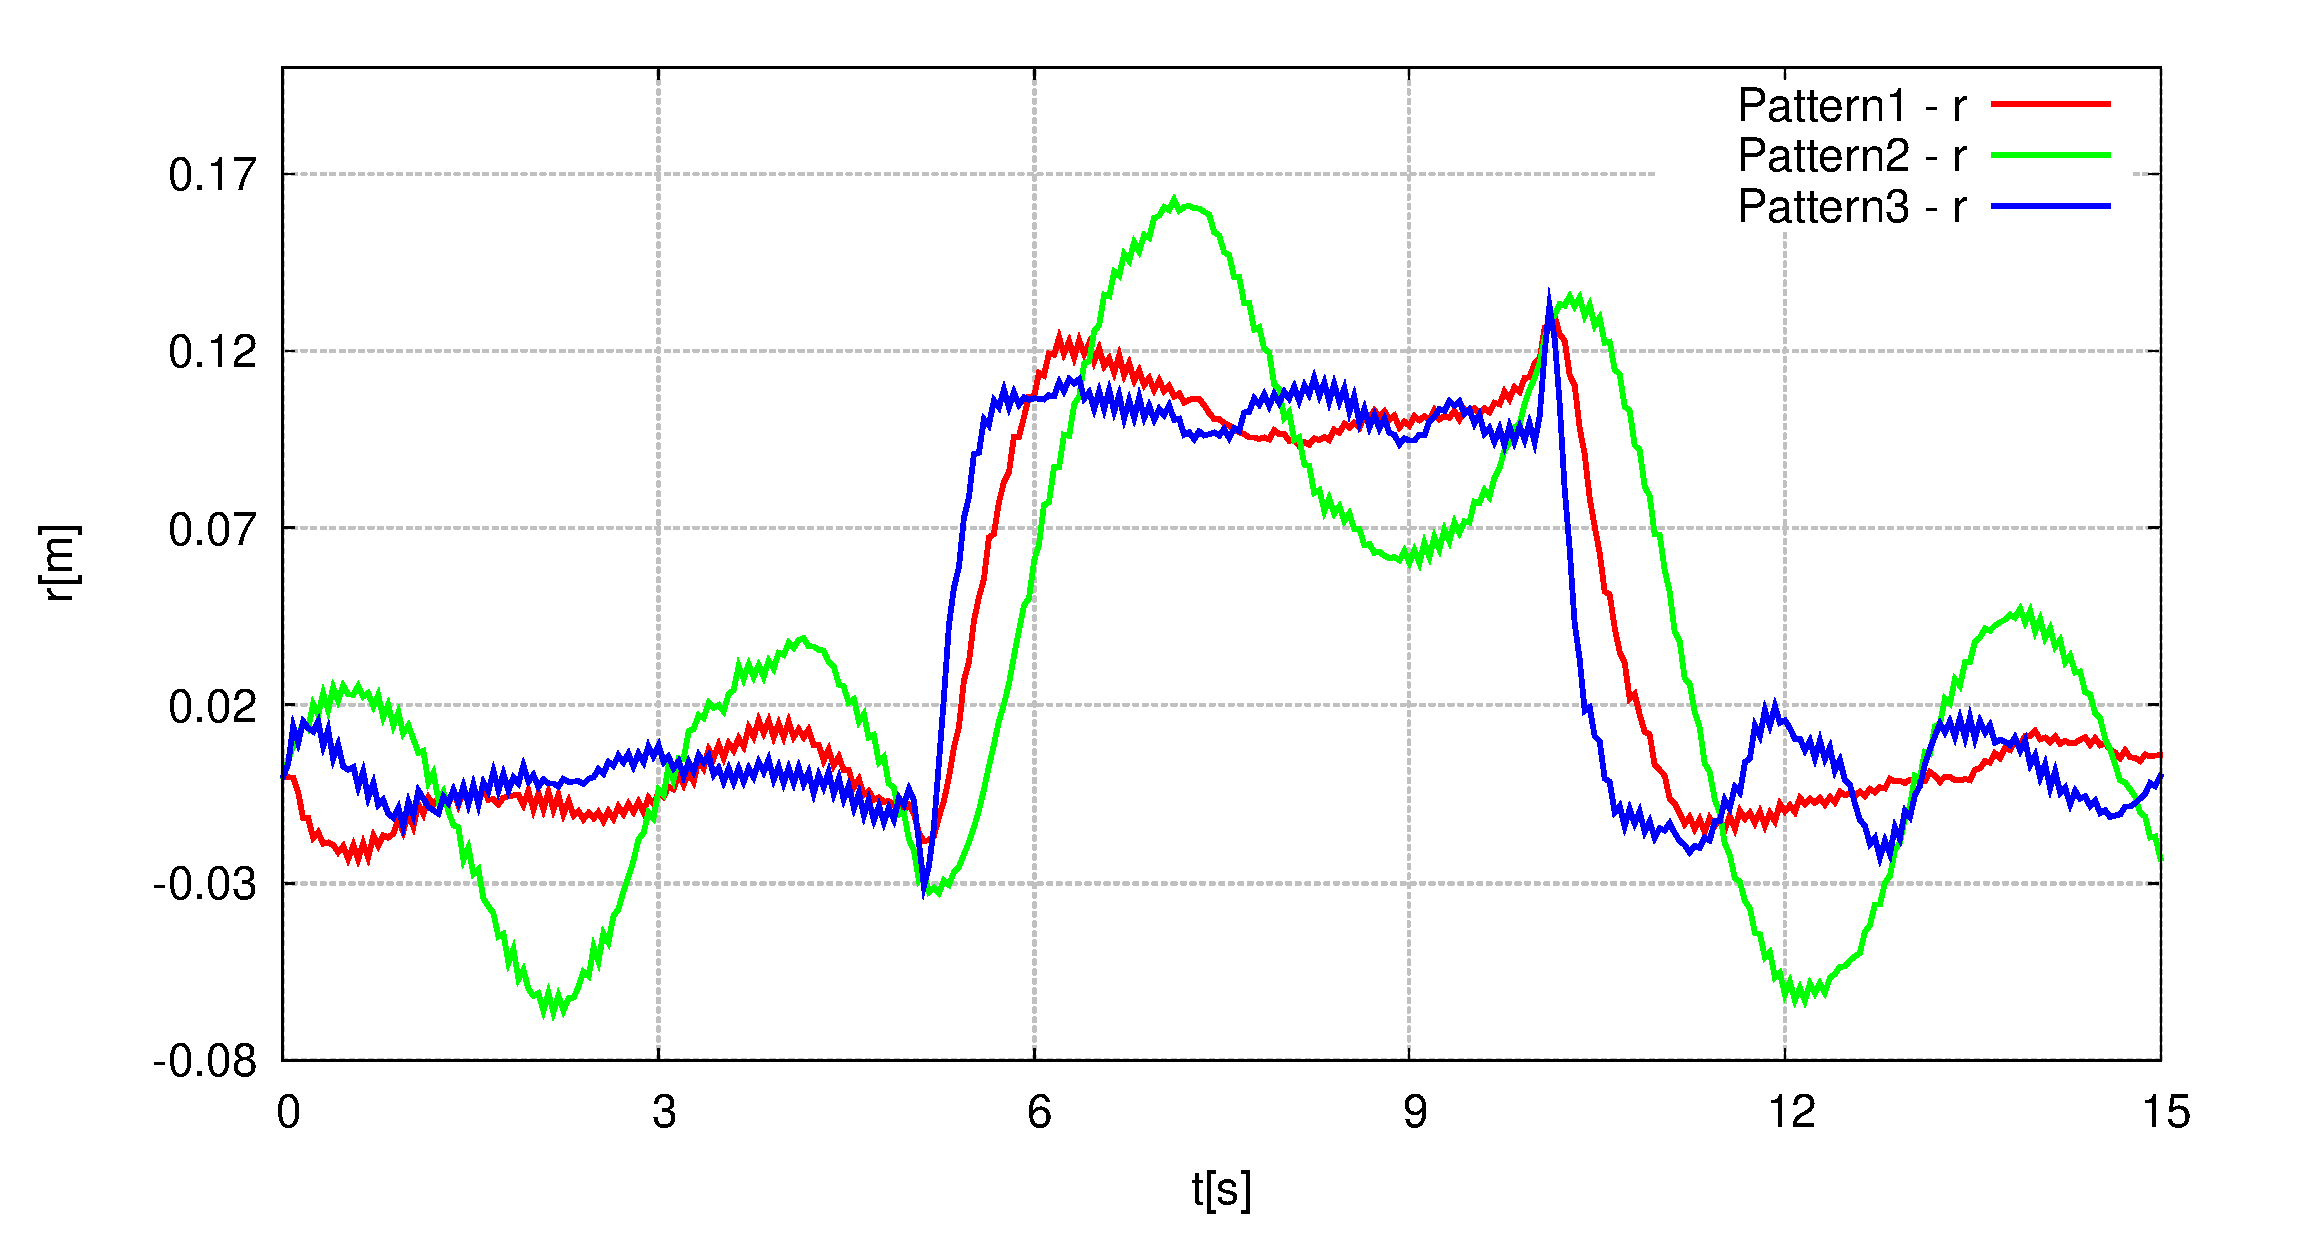
\includegraphics[width=0.49\linewidth]{gazo/Compare_Q_R2.eps}
		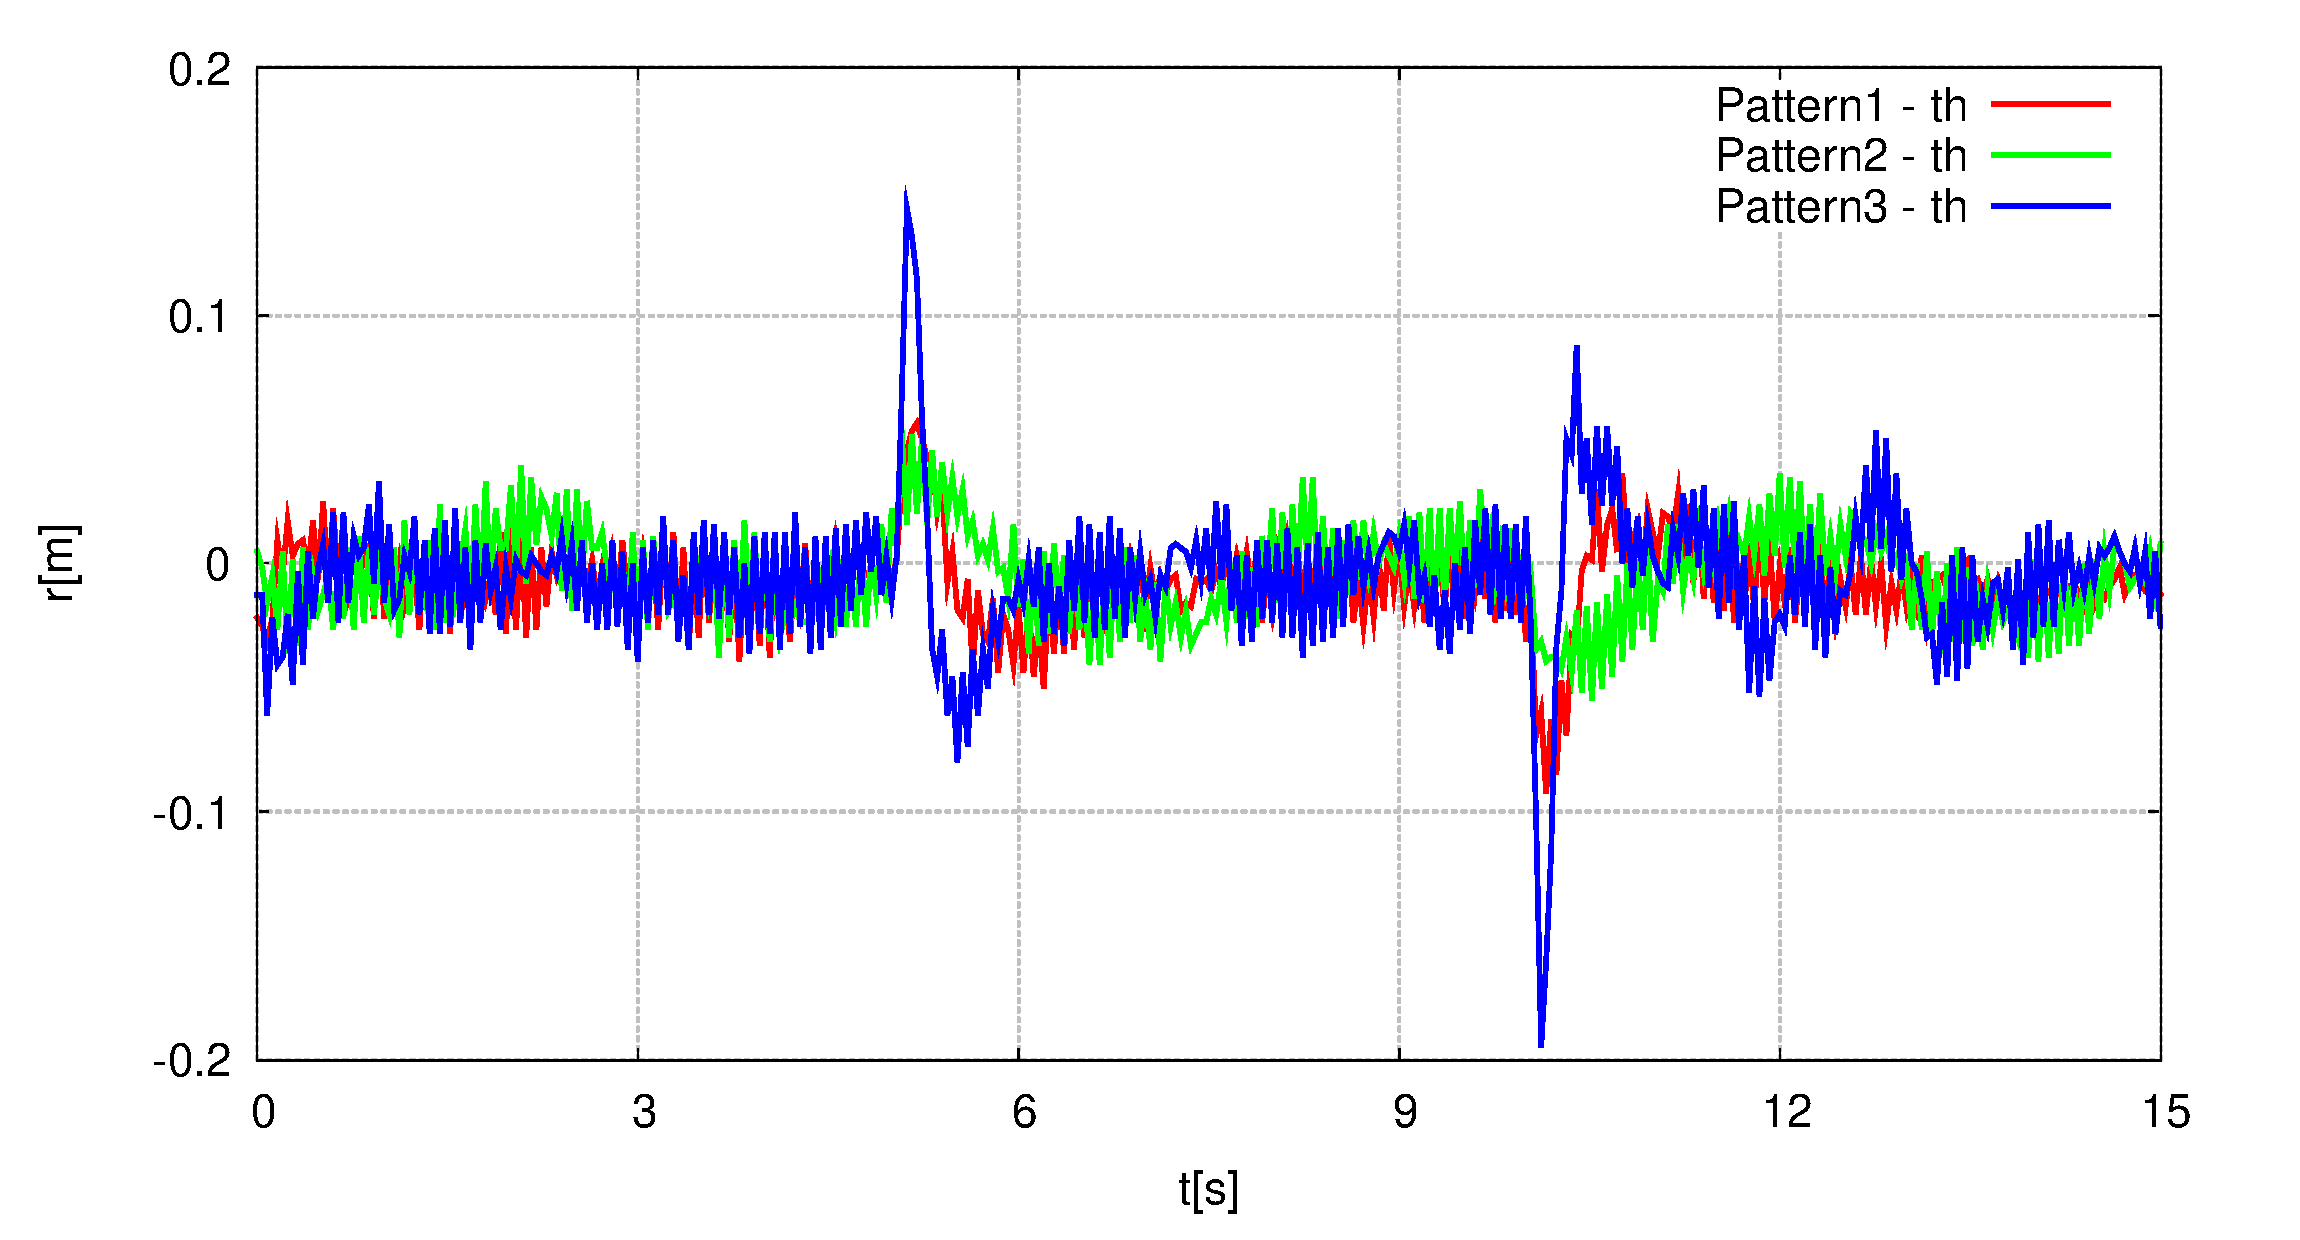
\includegraphics[width=0.49\linewidth]{gazo/Compare_Q_TH2.eps}
		\caption{重み行列の違いによる実験結果の比較}
		\label{image:comp_Q}
	\end{figure}
	図中のPatternは以下の表に対応するパラメータである。
	\begin{table}[H]
		\begin{center}
			\caption{パターンとパラメータの対応表}
			\medskip
			
			\begin{tabular}{|c|c|c|c|}\hline
				パターン & 重み行列$Q$ & オブザーバの極$P$ & サンプリング周期$\Delta[\rm{s}]$ \\ \hline\hline
				Pattern1 & $Q_1$:$\rm{diag}(1E5,1E5,1,1)$ & $P_1$:$((-30,0),(-30,0))^{'}$ & $\Delta_1$:0.005 \\ \hline
				Pattern2 & $Q_1$:$\rm{diag}(1E5,1E6,1,1)$ & $P_1$:$((-30,0),(-30,0))^{'}$ & $\Delta_1$:0.005 \\ \hline
				Pattern3 & $Q_1$:$\rm{diag}(1E6,1E5,1,1)$ & $P_1$:$((-30,0),(-30,0))^{'}$ & $\Delta_1$:0.005 \\ \hline
			\end{tabular}
		\end{center}
		\label{table:huriage_control}
	\end{table}
	図\ref{image:comp_Q}の左図を見えると、台車の位置に関しては、パターン3→パターン1→パターン2の順に応答が遅くなっていることがわかる。
	特にパターン2の方は目標値変更に対して台車が移動してはいるが、波打って動いていることがわかる。つまり、
	重み行列の第一成分を大きくしているパターン3の応答が一番よく、重み行列の第二成分を大きくしたパターン2
	はバランスがくずれてしまい応答が一番悪いといえる。
	右図の振子の角度についても同様のことが言える。パターン3は台車が動く時に角度が大きく傾いてしまっているが、パターン2は台車が動く時においても、大きな角度の傾きは確認できない。
	つまり、重み行列の第二成分を大きくしているパターン2の応答が一番よく、重み行列の第一成分を大きくしたパターン3は
	バランスが崩れてしまい応答が一番悪いといえる。
	シミュレーションの章でも述べたように重み行列の各成分は各状態に対応しており、応答を良くしたい状態があれば、それに対応する
	成分をおおきくすればよいということが実験でも確認できる。
	\par
	%--------------------------------------------------------------------------------------------------------
	\subsection{オブザーバの極の違いによる実験結果の比較}
	次にオブザーバの極の違いによる実験結果の比較を見てみる。
	\begin{figure}[H]
		\centering
		\includegraphics[width=0.49\linewidth]{gazo/Compare_obs_R2.eps}
		\includegraphics[width=0.49\linewidth]{gazo/Compare_obs_TH2.eps}
		\caption{オブザーバの極の違いによる実験結果の比較}
		\label{image:comp_obs}
	\end{figure}
	図中のPatternは以下の表に対応するパラメータである。
	\begin{table}[H]
		\begin{center}
			\caption{パターンとパラメータの対応表}
			\medskip
			
			\begin{tabular}{|c|c|c|c|}\hline
				パターン & 重み行列$Q$ & オブザーバの極$P$ & サンプリング周期$\Delta[\rm{s}]$ \\ \hline\hline
				Pattern1 & $Q_1$:$\rm{diag}(1E5,1E5,1,1)$ & $P_1$:$((-30,0),(-30,0))^{'}$ & $\Delta_1$:0.005 \\ \hline
				Pattern2 & $Q_1$:$\rm{diag}(1E5,1E5,1,1)$ & $P_1$:$((-60,0),(-60,0))^{'}$ & $\Delta_1$:0.005 \\ \hline
			\end{tabular}
		\end{center}
		\label{table:huriage_control}
	\end{table}
	図\ref{image:comp_obs}の左図より、台車の位置についてはパターン1とパターン2において応答の速さで大きな違いはないといえる。
	しかし、台車の位置が0.1になったときのパターン2の波形はパターン1の波形と比べて振動的になっていいることがわかる。このことから、
	オブザーバーの極が虚軸から遠くなると応答は振動的になると考えられる。
	右図より、振子の角度については、パターン1とパターン2では大きな違いは確認できないといえる。
	\newpage
	%--------------------------------------------------------------------------------------------------
	\subsection{サンプリング周期の違いによる実験結果の比較}
	次にサンプリング周期の違いによる実験結果の比較を見てみる。
	\begin{figure}[H]
		\centering
		\includegraphics[width=0.49\linewidth]{gazo/Compare_dt_R2.eps}
		\includegraphics[width=0.49\linewidth]{gazo/Compare_dt_TH2.eps}
		\caption{サンプリング周期の違いによる実験結果の比較}
		\label{image:comp_dt}
	\end{figure}
	図中のPatternは以下の表に対応するパラメータである。
	\begin{table}[H]
		\begin{center}
			\caption{パターンとパラメータの対応表}
			\medskip
			
			\begin{tabular}{|c|c|c|c|}\hline
				パターン & 重み行列$Q$ & オブザーバの極$P$ & サンプリング周期$\Delta[\rm{s}]$ \\ \hline\hline
				Pattern1 & $Q_1$:$\rm{diag}(1E5,1E5,1,1)$ & $P_1$:$((-30,0),(-30,0))^{'}$ & $\Delta_1$:0.005 \\ \hline
				Pattern2 & $Q_1$:$\rm{diag}(1E5,1E5,1,1)$ & $P_1$:$((-30,0),(-30,0))^{'}$ & $\Delta_1$:0.010 \\ \hline
			\end{tabular}
		\end{center}
		\label{table:huriage_control}
	\end{table}
	図\ref{image:comp_dt}の左図より、台車の位置についてはサンプリング周期が長い方のパターン2の方が0.1に移動した際の台車の位置と0に移動する直前の台車の位置に大きな
	ズレがないことがわかる。これはサンプリング周期が長いため台車の動きが緩やかになったためと考える。右図より、振子の角度については
	目標値が0に戻る時点での角度のズレがパターン2の方が小さいことがわかる。台車の位置が大きくズレなかった結果、振子の角度のズレも小さくなったといえるが、
	サンプリング周期が長い影響であるともいえる。つまり、サンプリング周期が長くなったことで、拾いきれない情報が存在し、台車の動きが緩やかになったといえる。
	\newpage
	%---------------------------------------------------------------------------------------------------------
	\subsection{シミュレーション結果と実験結果の比較}
	以下に実験結果とシミュレーション結果との比較を行った図を示す。
	また、図の数が多いので図のキャプションとその図における各パラメータの対応表を示す。
	\begin{table}[H]
		\begin{center}
			\caption{図に対応するパラメータの組}
			\begin{tabular}{|c|c|c|c|}\hline
				図のキャプション & 重み行列$Q$ & オブザーバの極$P$ & サンプリング周期$\Delta[\rm{s}]$ \\ \hline\hline
				比較結果その1 & $Q_1$:$\rm{diag}(1E5,1E5,1,1)$ & $P_1$:$((-30,0),(-30,0))^{'}$ & $\Delta_1$:0.005 \\ \hline
				比較結果その2 & $Q_1$:$\rm{diag}(1E5,1E6,1,1)$ & $P_1$:$((-30,0),(-30,0))^{'}$ & $\Delta_1$:0.005 \\ \hline
				比較結果その3 & $Q_1$:$\rm{diag}(1E6,1E5,1,1)$ & $P_1$:$((-30,0),(-30,0))^{'}$ & $\Delta_1$:0.005 \\ \hline
				比較結果その4 & $Q_1$:$\rm{diag}(1E5,1E5,1,1)$ & $P_1$:$((-60,0),(-60,0))^{'}$ & $\Delta_1$:0.005 \\ \hline
				比較結果その5 & $Q_1$:$\rm{diag}(1E5,1E6,1,1)$ & $P_1$:$((-60,0),(-60,0))^{'}$ & $\Delta_1$:0.005 \\ \hline
				比較結果その6 & $Q_1$:$\rm{diag}(1E6,1E5,1,1)$ & $P_1$:$((-60,0),(-60,0))^{'}$ & $\Delta_1$:0.005 \\ \hline
				比較結果その7 & $Q_1$:$\rm{diag}(1E5,1E5,1,1)$ & $P_1$:$((-30,0),(-30,0))^{'}$ & $\Delta_1$:0.010 \\ \hline
				比較結果その8 & $Q_1$:$\rm{diag}(1E5,1E6,1,1)$ & $P_1$:$((-30,0),(-30,0))^{'}$ & $\Delta_1$:0.010 \\ \hline
				比較結果その9 & $Q_1$:$\rm{diag}(1E6,1E5,1,1)$ & $P_1$:$((-30,0),(-30,0))^{'}$ & $\Delta_1$:0.010 \\ \hline
				比較結果その10 & $Q_1$:$\rm{diag}(1E5,1E5,1,1)$ & $P_1$:$((-60,0),(-60,0))^{'}$ & $\Delta_1$:0.010 \\ \hline
				比較結果その11 & $Q_1$:$\rm{diag}(1E5,1E6,1,1)$ & $P_1$:$((-60,0),(-60,0))^{'}$ & $\Delta_1$:0.010 \\ \hline
				比較結果その12 & $Q_1$:$\rm{diag}(1E6,1E5,1,1)$ & $P_1$:$((-60,0),(-60,0))^{'}$ & $\Delta_1$:0.010 \\ \hline
			\end{tabular}
		\end{center}
		\label{table:huriage_control}
	\end{table}
	
	\begin{figure}[H]
		\centering
		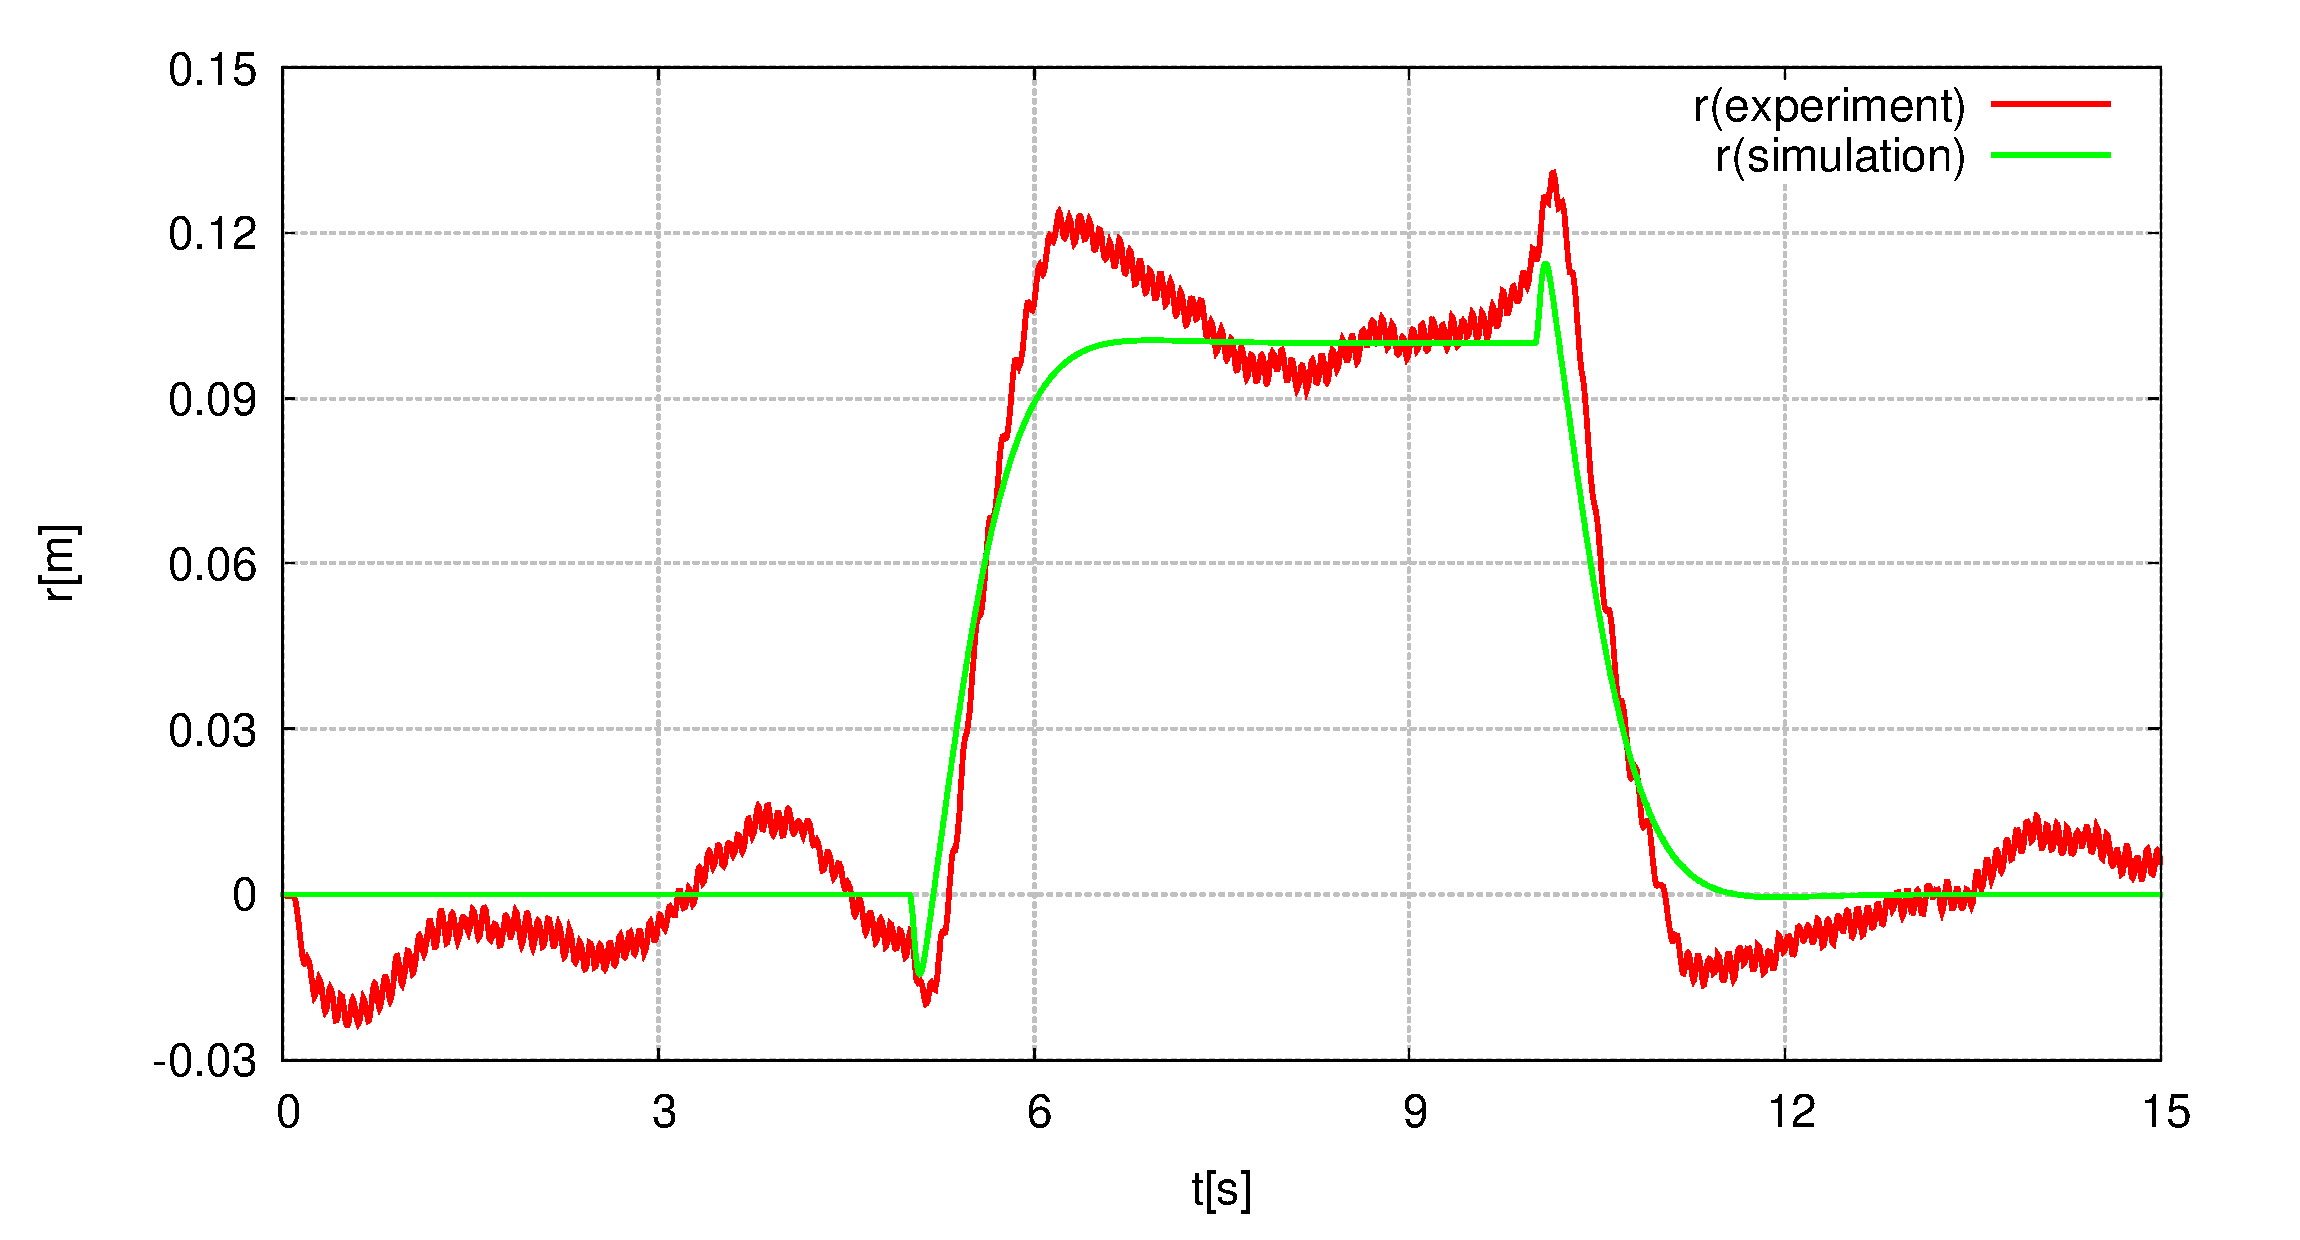
\includegraphics[width=0.49\linewidth]{gazo/experiment_Q55obs30dt05R2.eps}
		\includegraphics[width=0.49\linewidth]{gazo/experiment_Q55obs30dt05TH2.eps}
		\caption{比較結果その1(左図がr,右図が$\theta$)}
		\label{image:sono1}
	\end{figure}
	\begin{figure}[H]
		\centering
		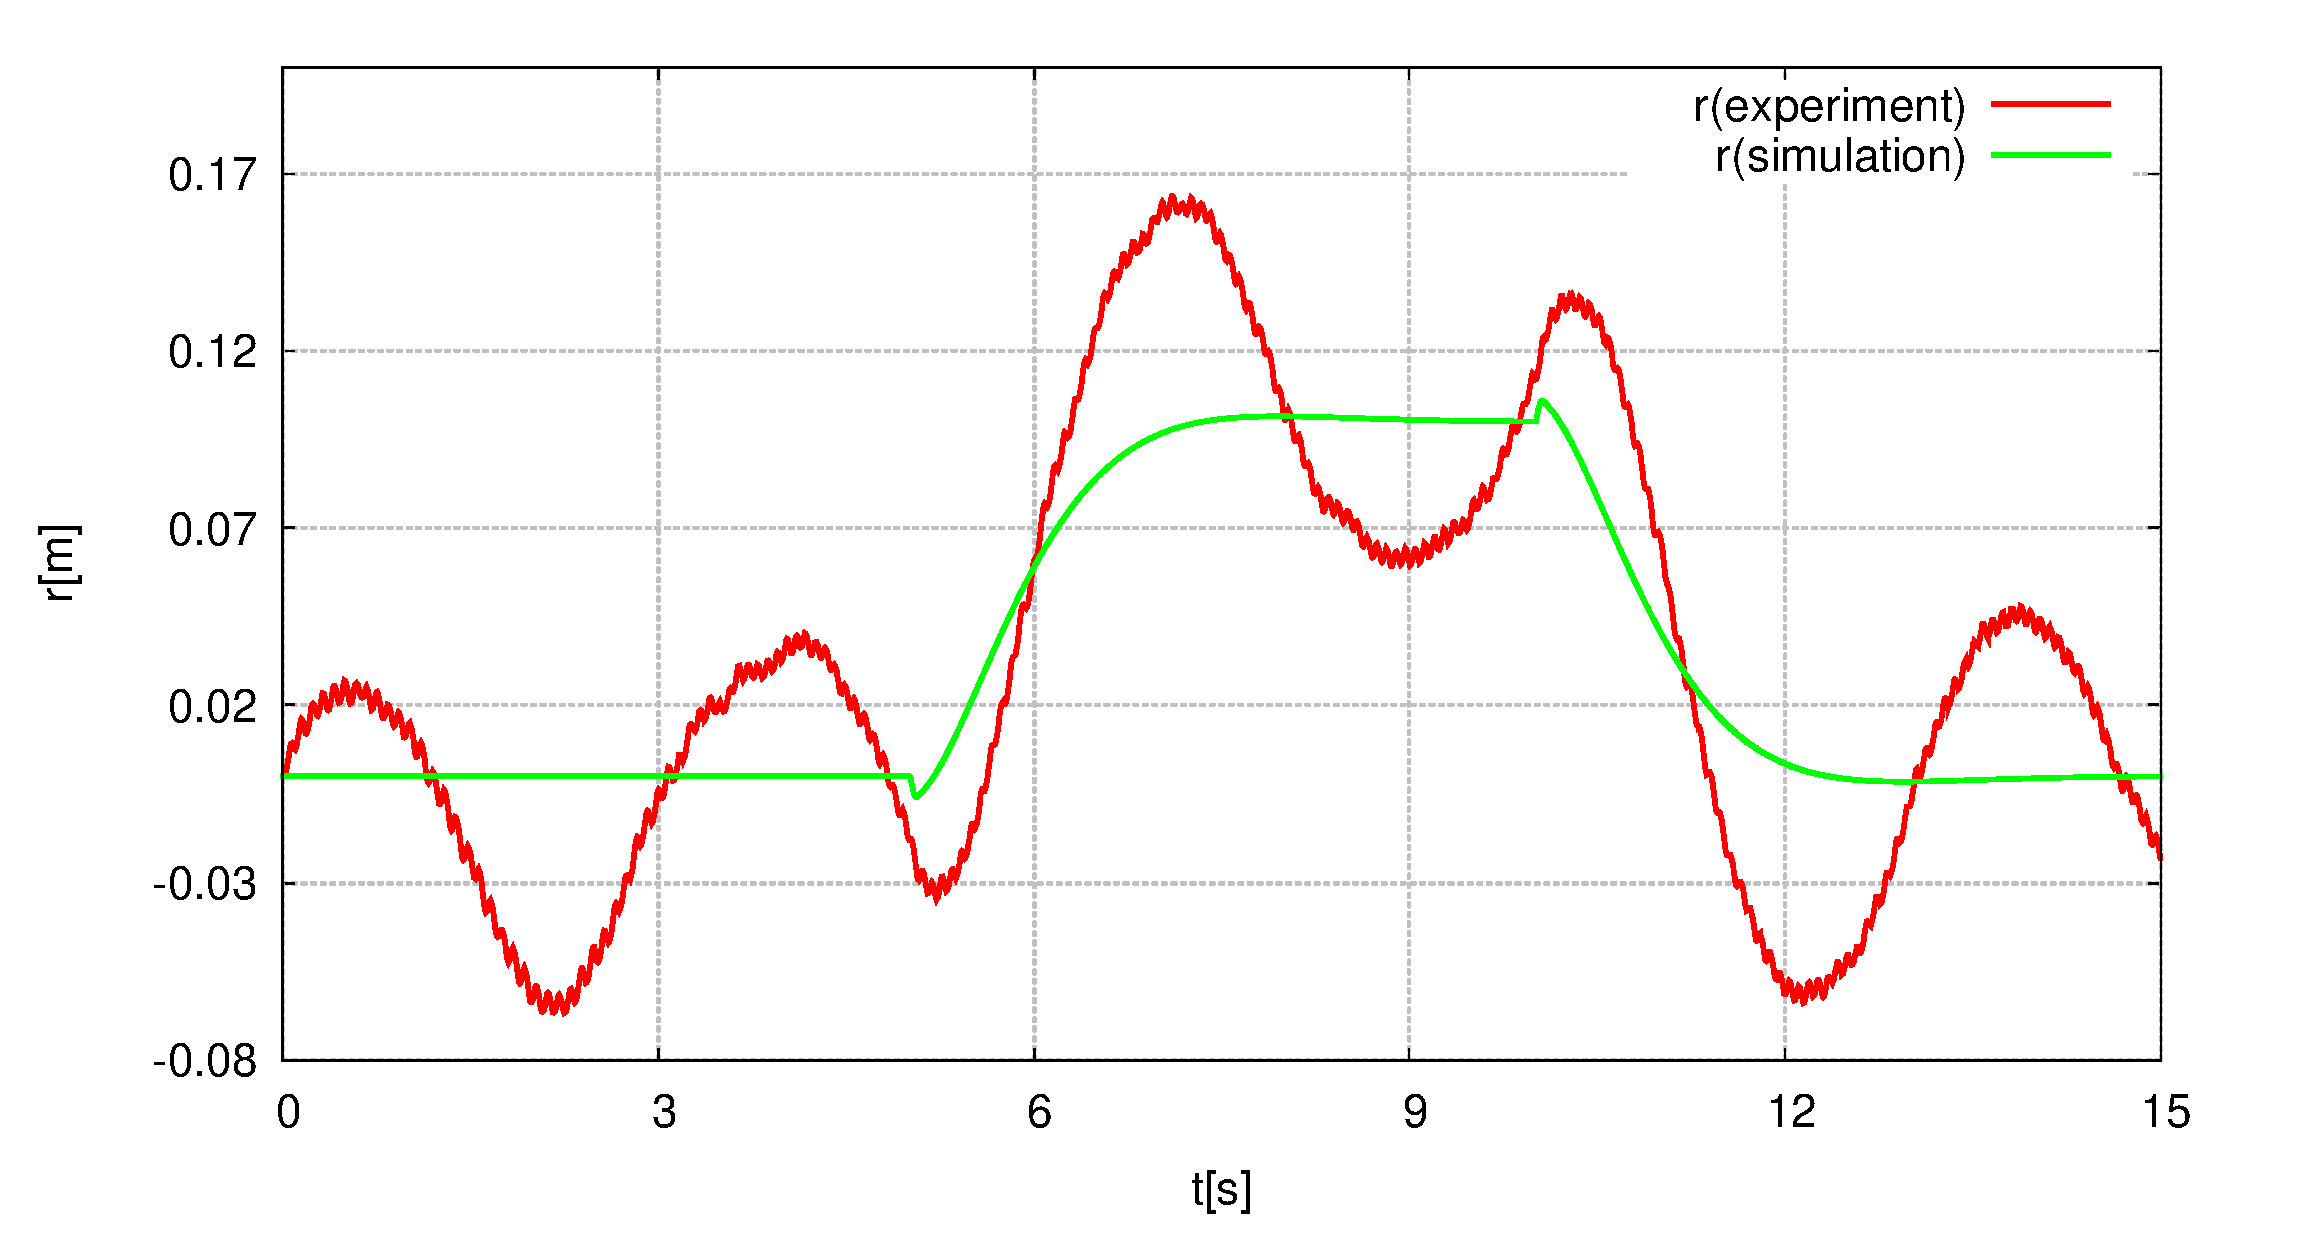
\includegraphics[width=0.49\linewidth]{gazo/experiment_Q56obs30dt05R2.eps}
		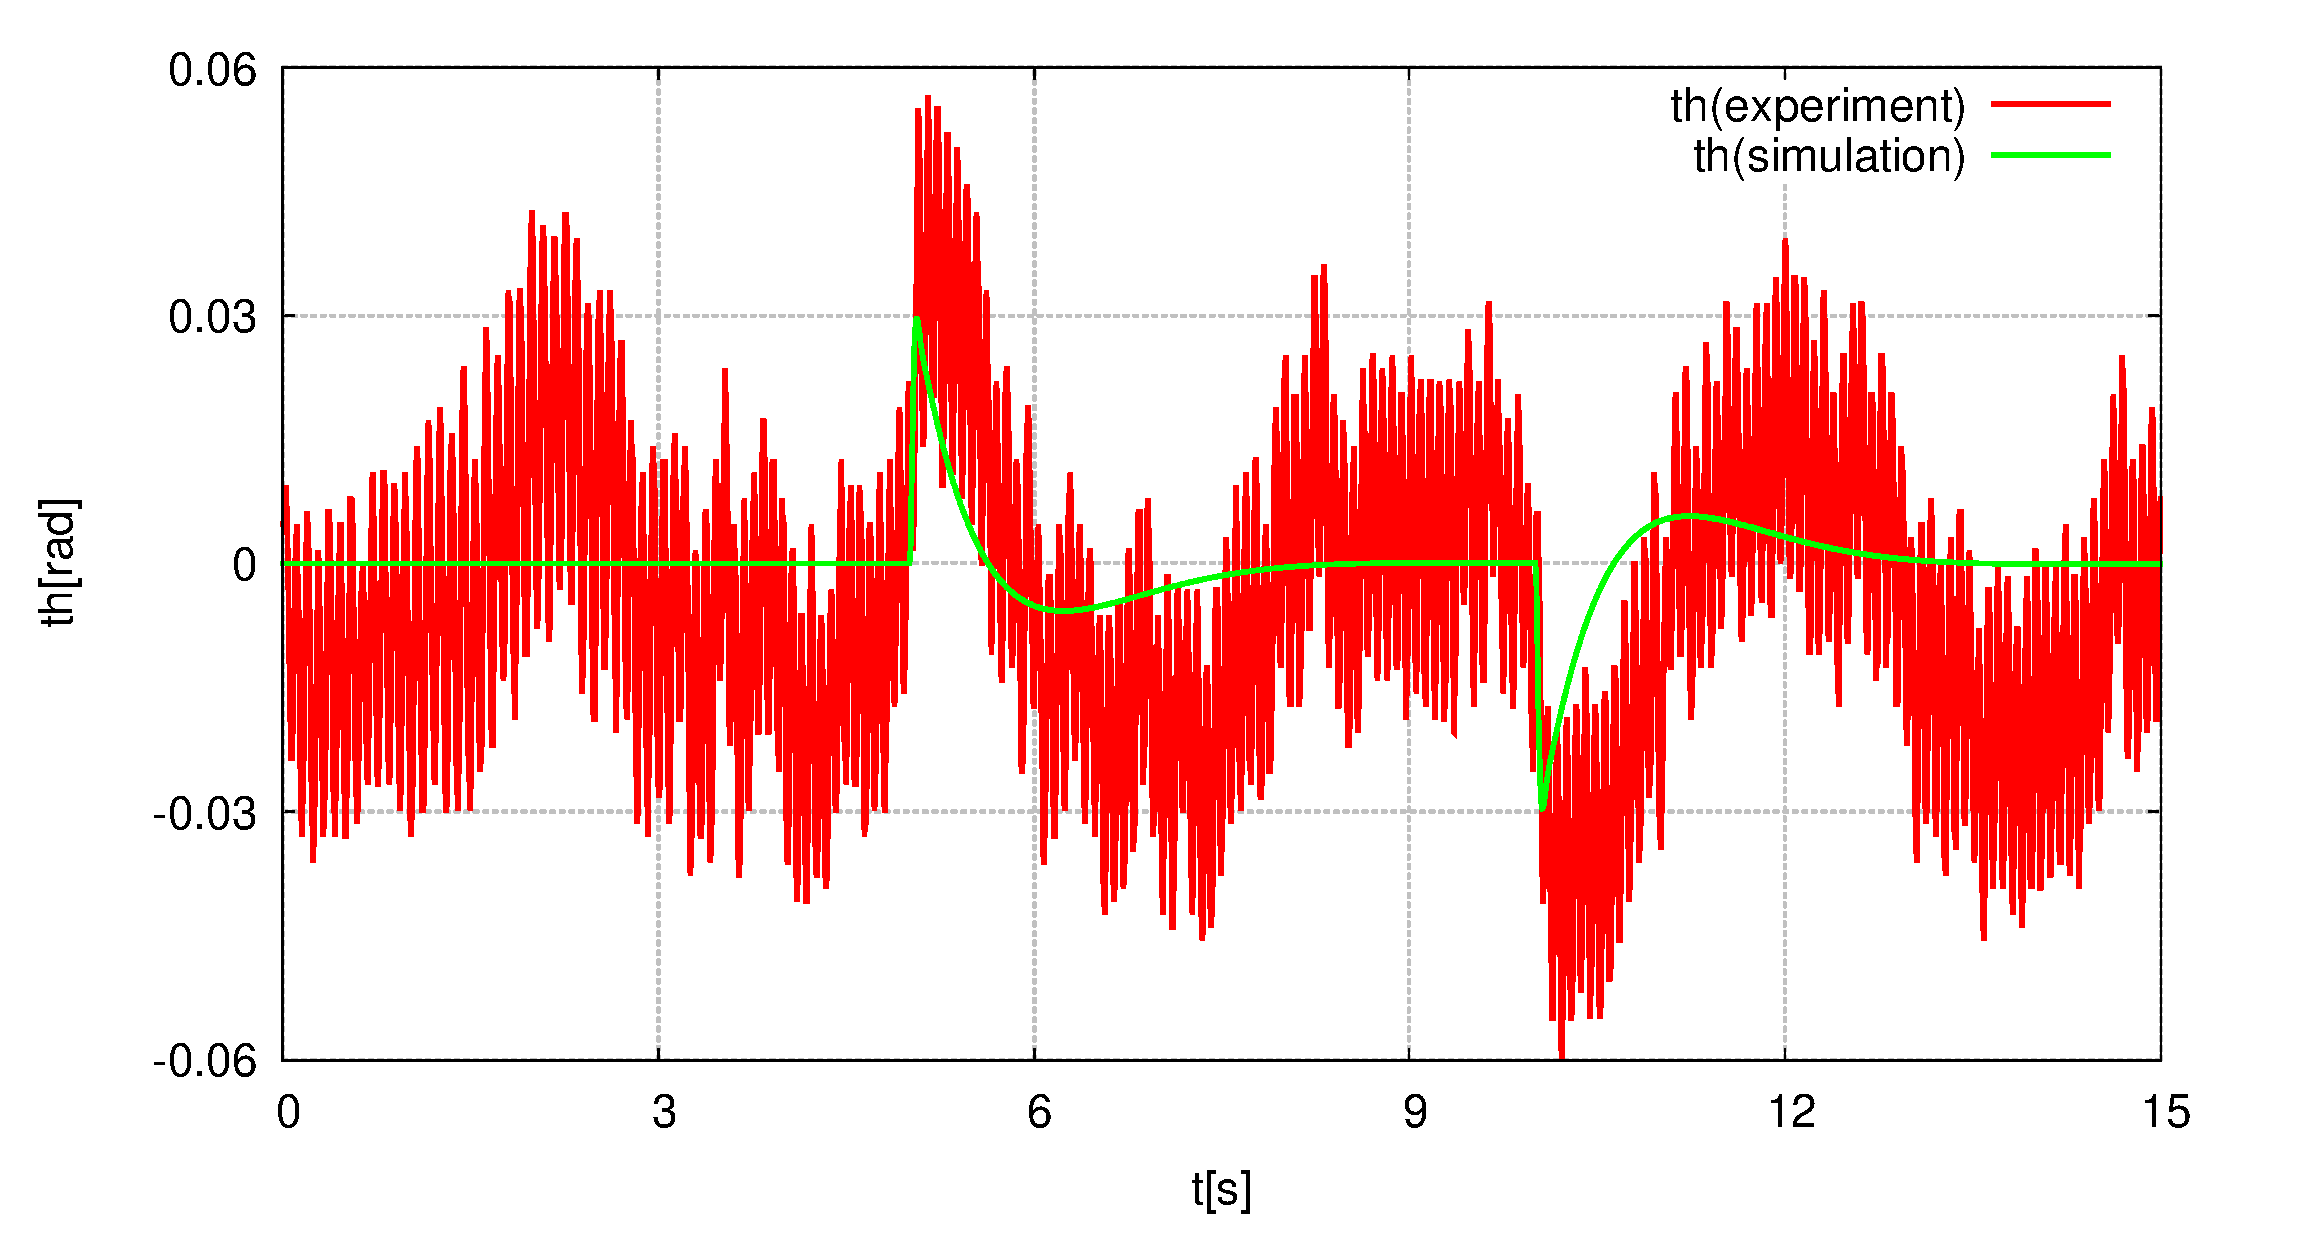
\includegraphics[width=0.49\linewidth]{gazo/experiment_Q56obs30dt05TH2.eps}
		\caption{比較結果その2(左図がr,右図が$\theta$)}
		\label{image:sono2}
	\end{figure}
	\begin{figure}[H]
		\centering
		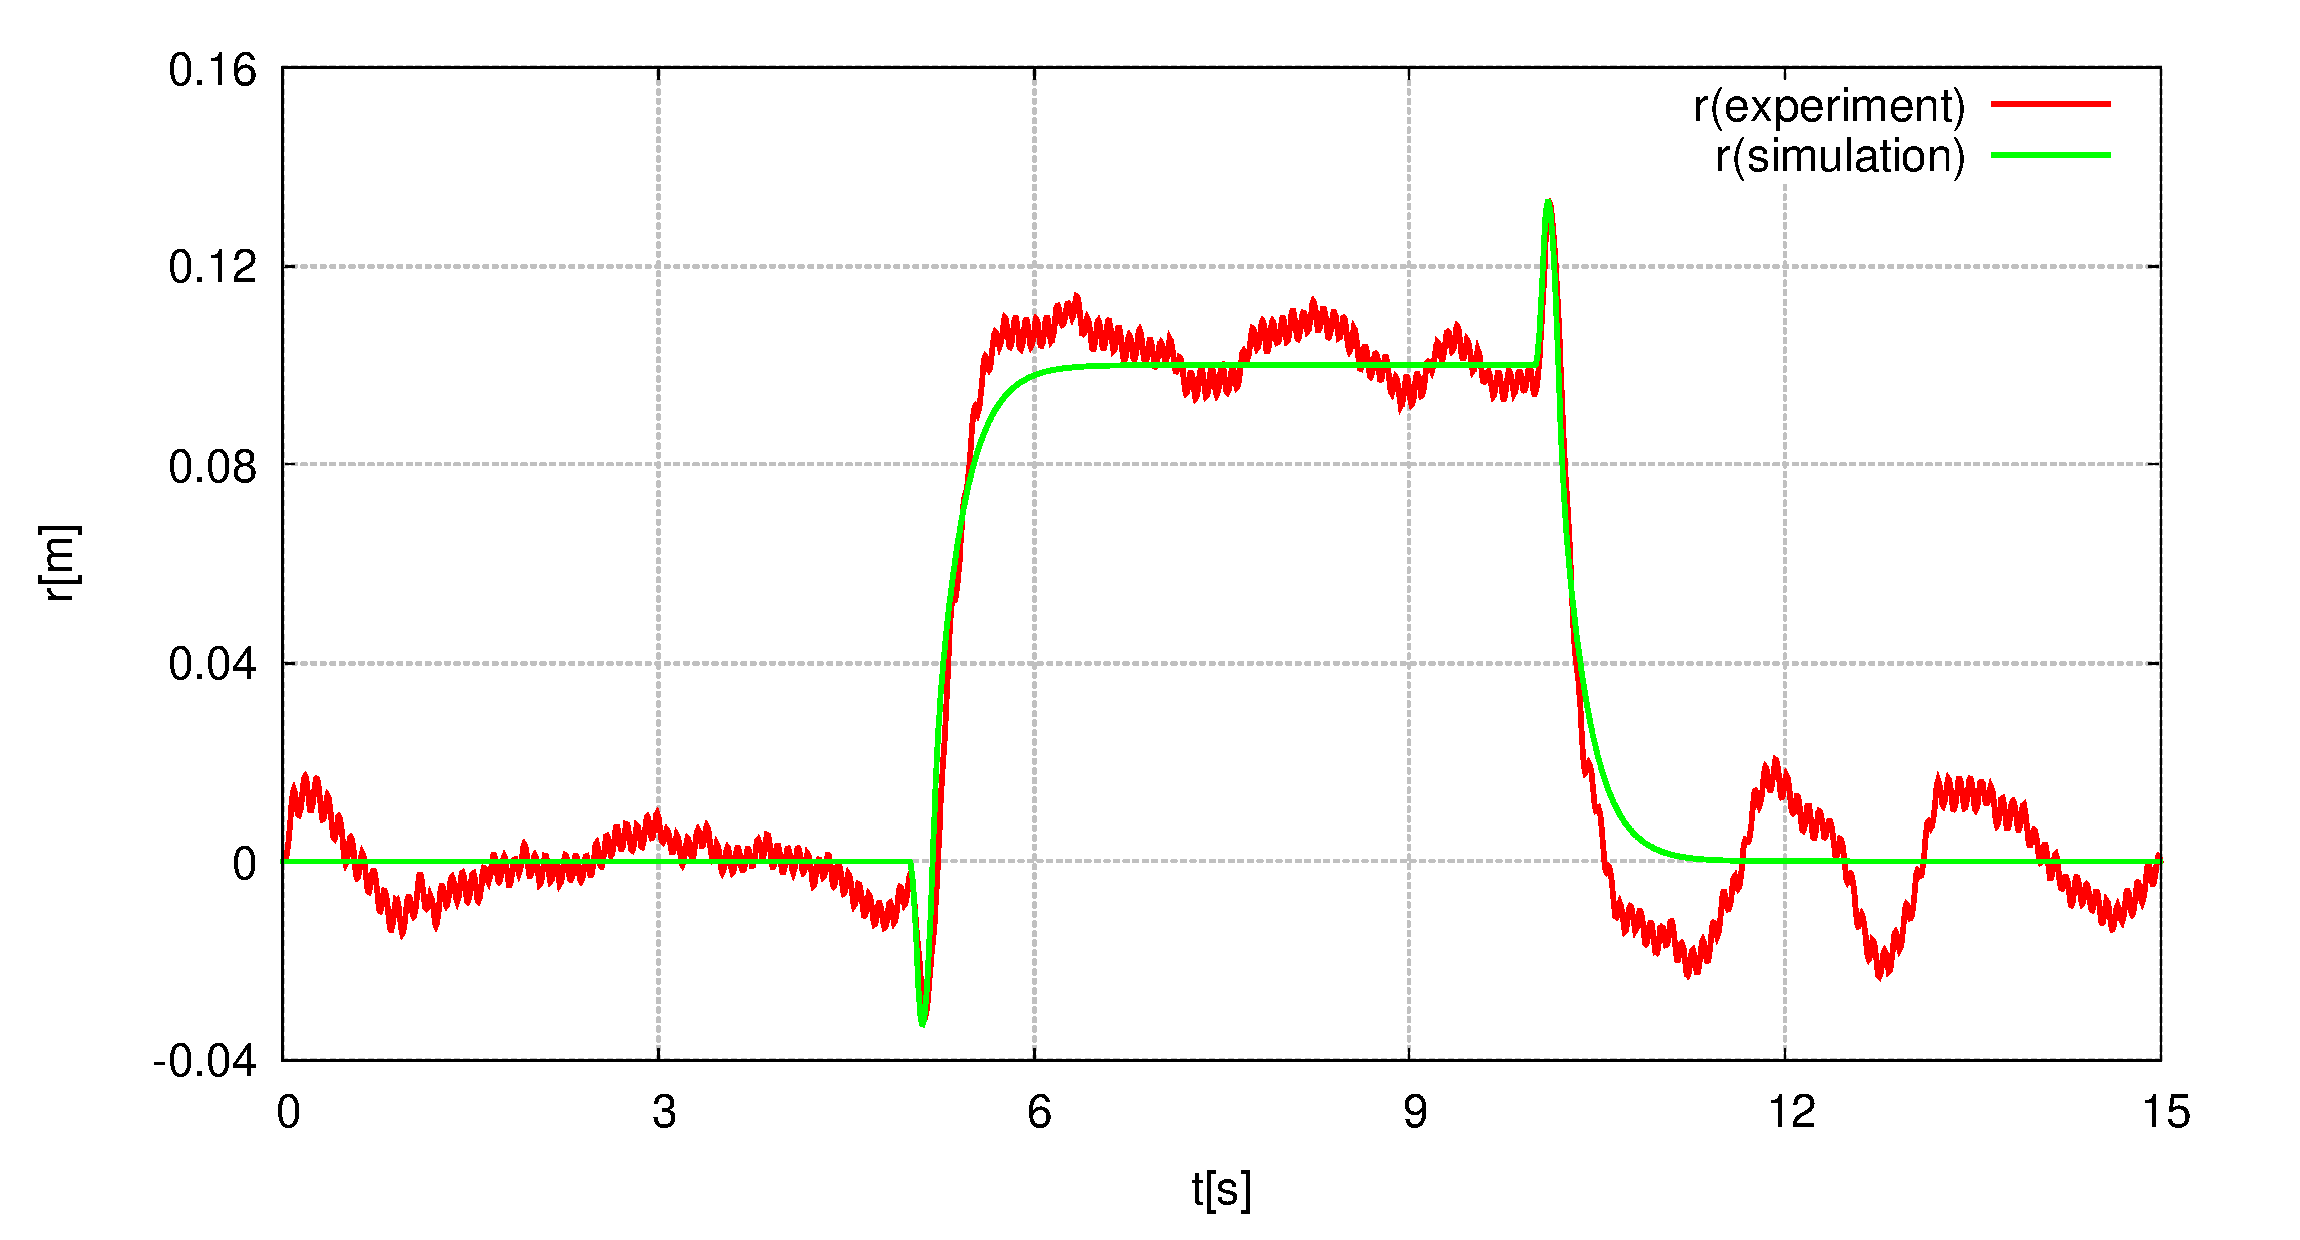
\includegraphics[width=0.49\linewidth]{gazo/experiment_Q65obs30dt05R2.eps}
		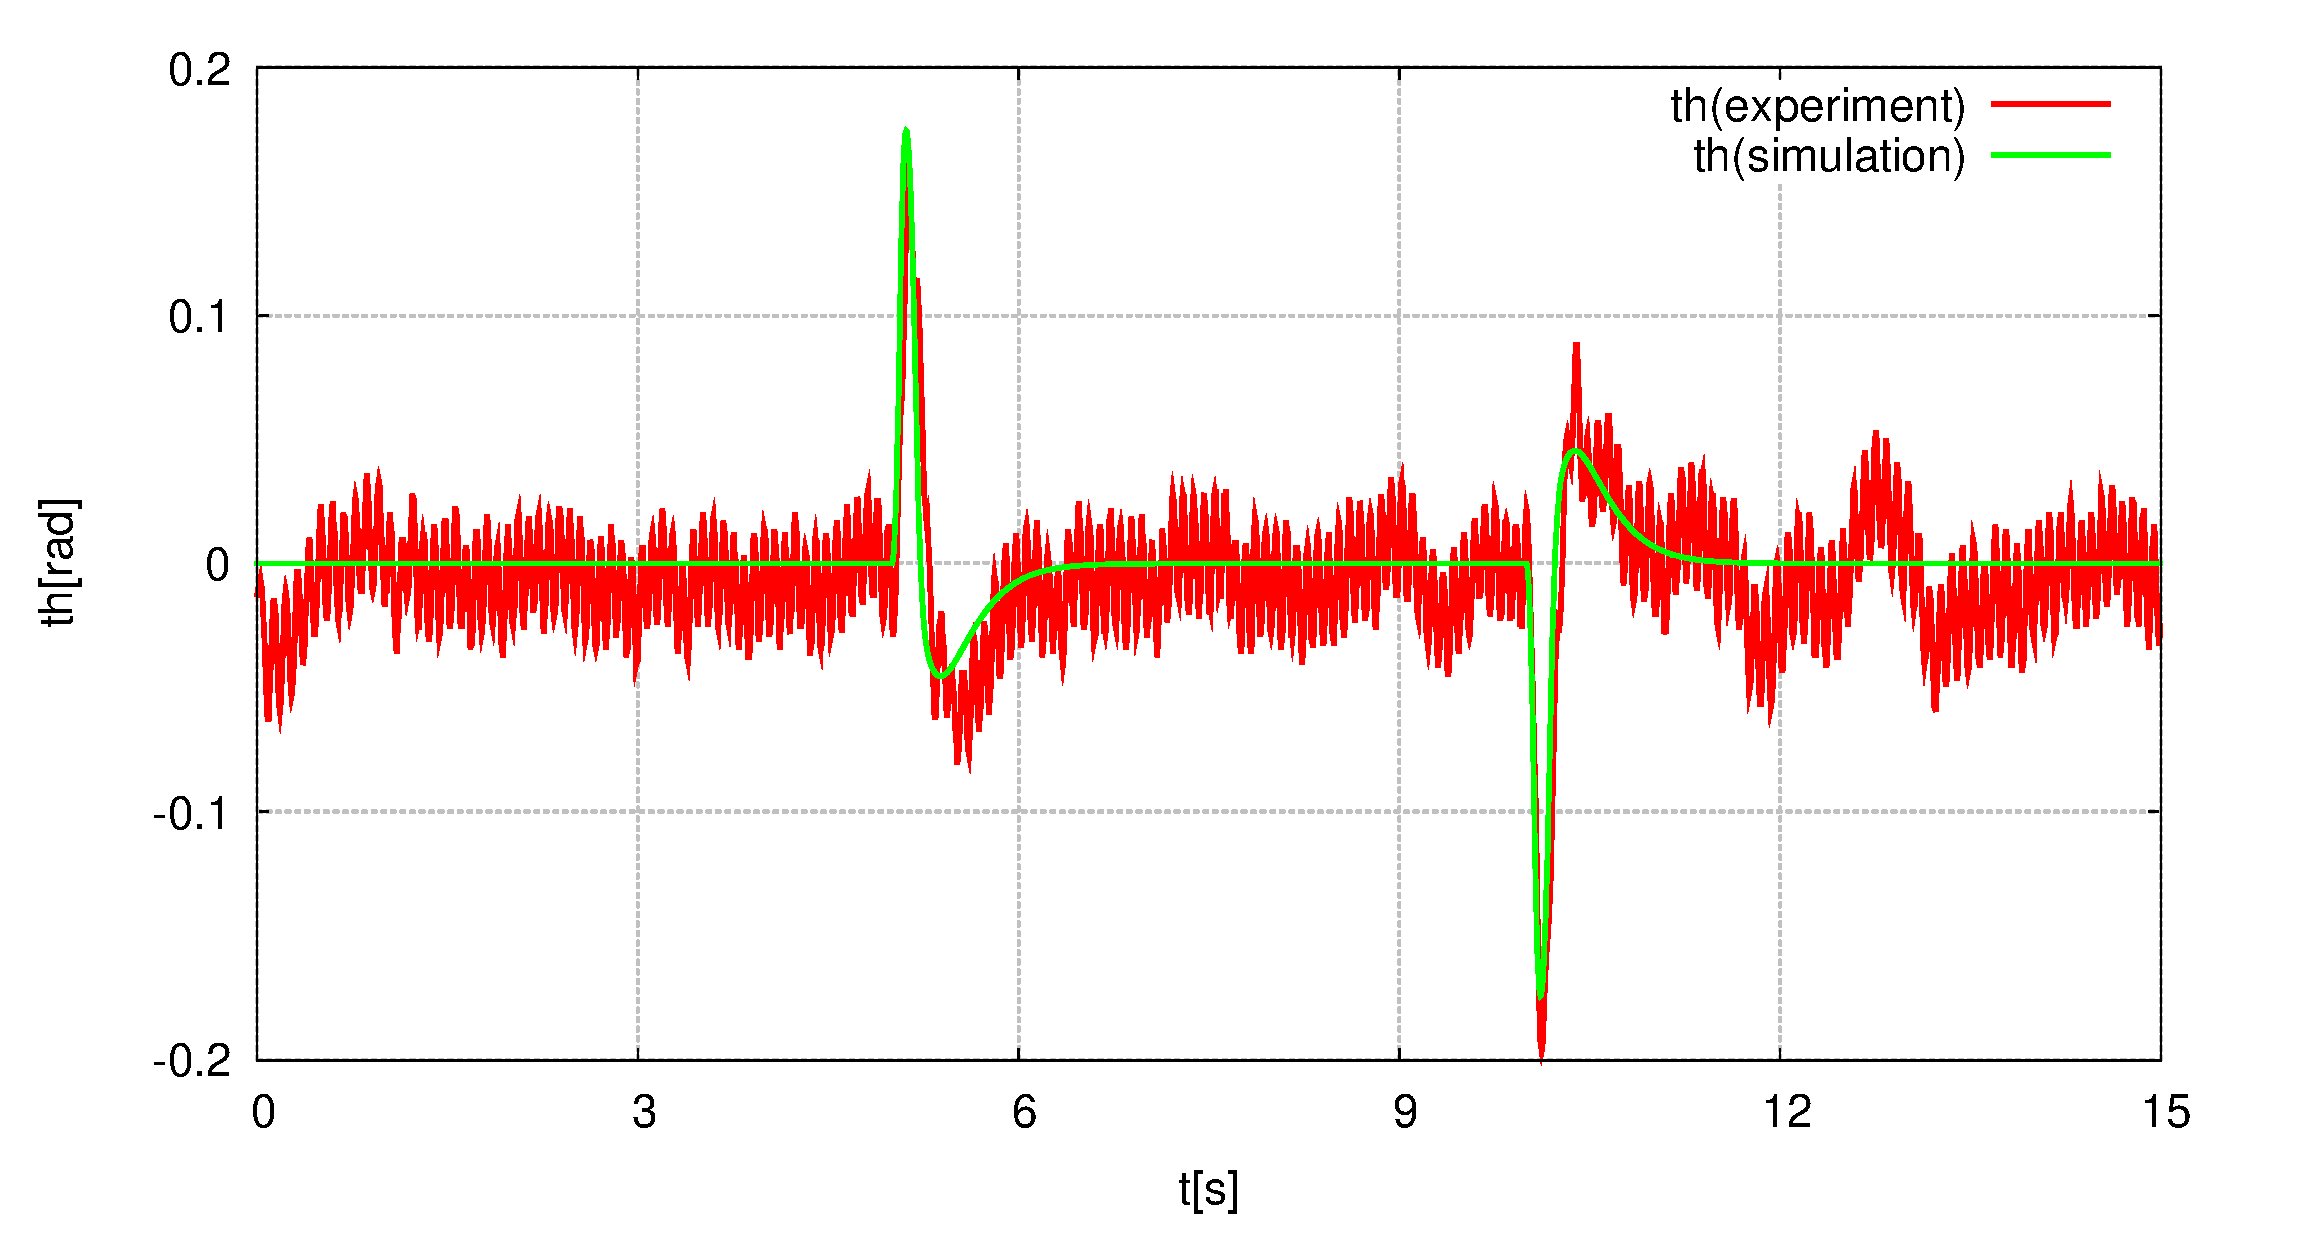
\includegraphics[width=0.49\linewidth]{gazo/experiment_Q65obs30dt05TH2.eps}
		\caption{比較結果その3(左図がr,右図が$\theta$)}
		\label{image:sono3}
	\end{figure}
	\begin{figure}[H]
		\centering
		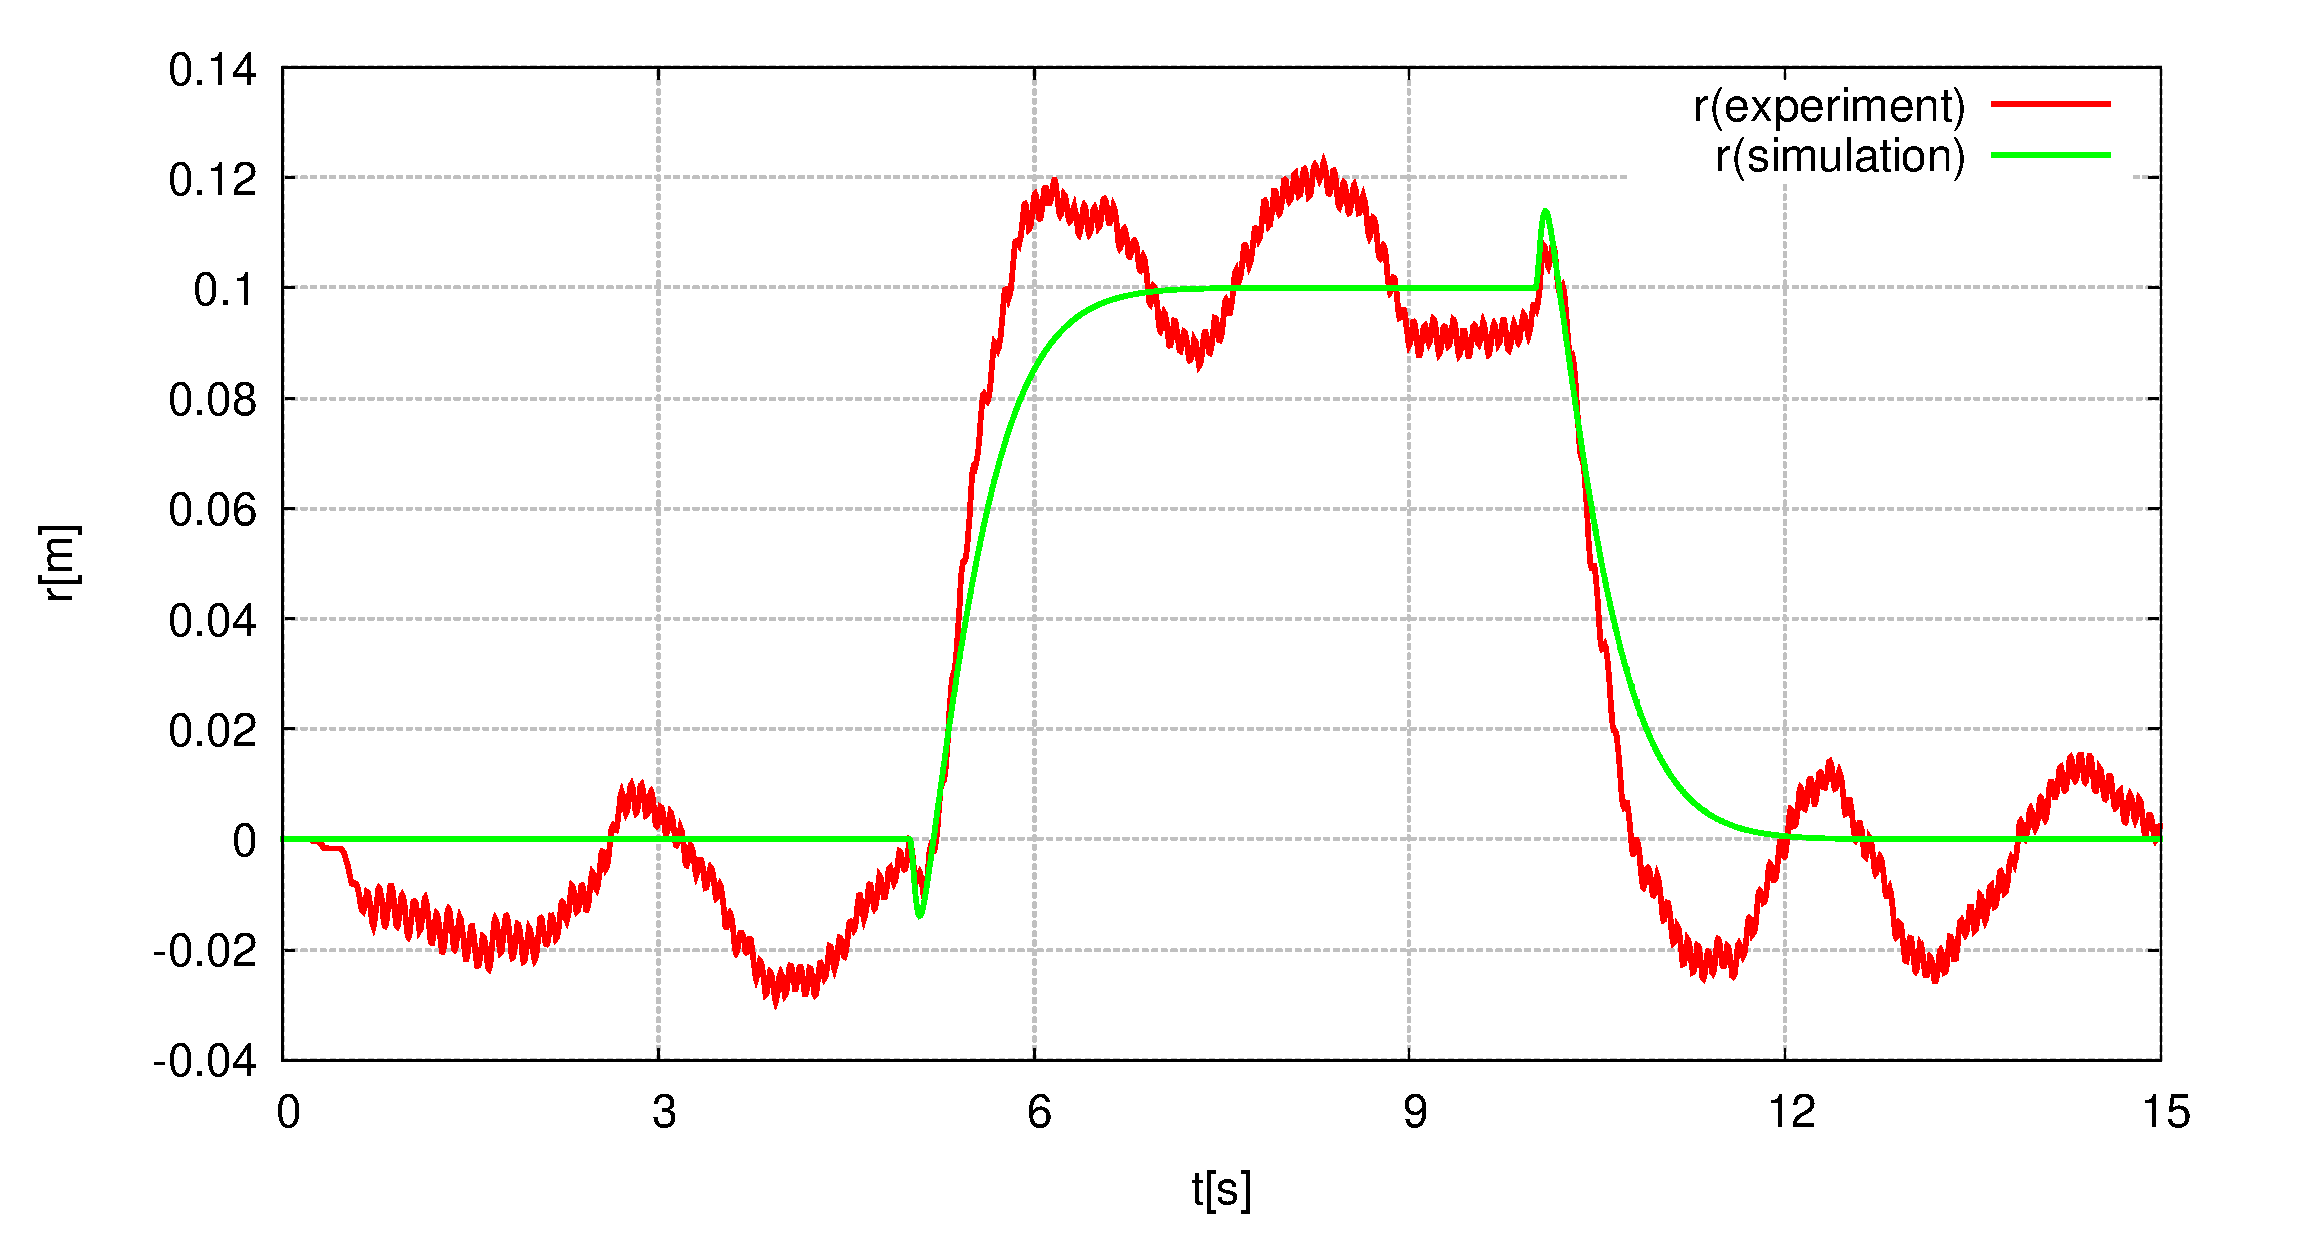
\includegraphics[width=0.49\linewidth]{gazo/experiment_Q55obs60dt05R2.eps}
		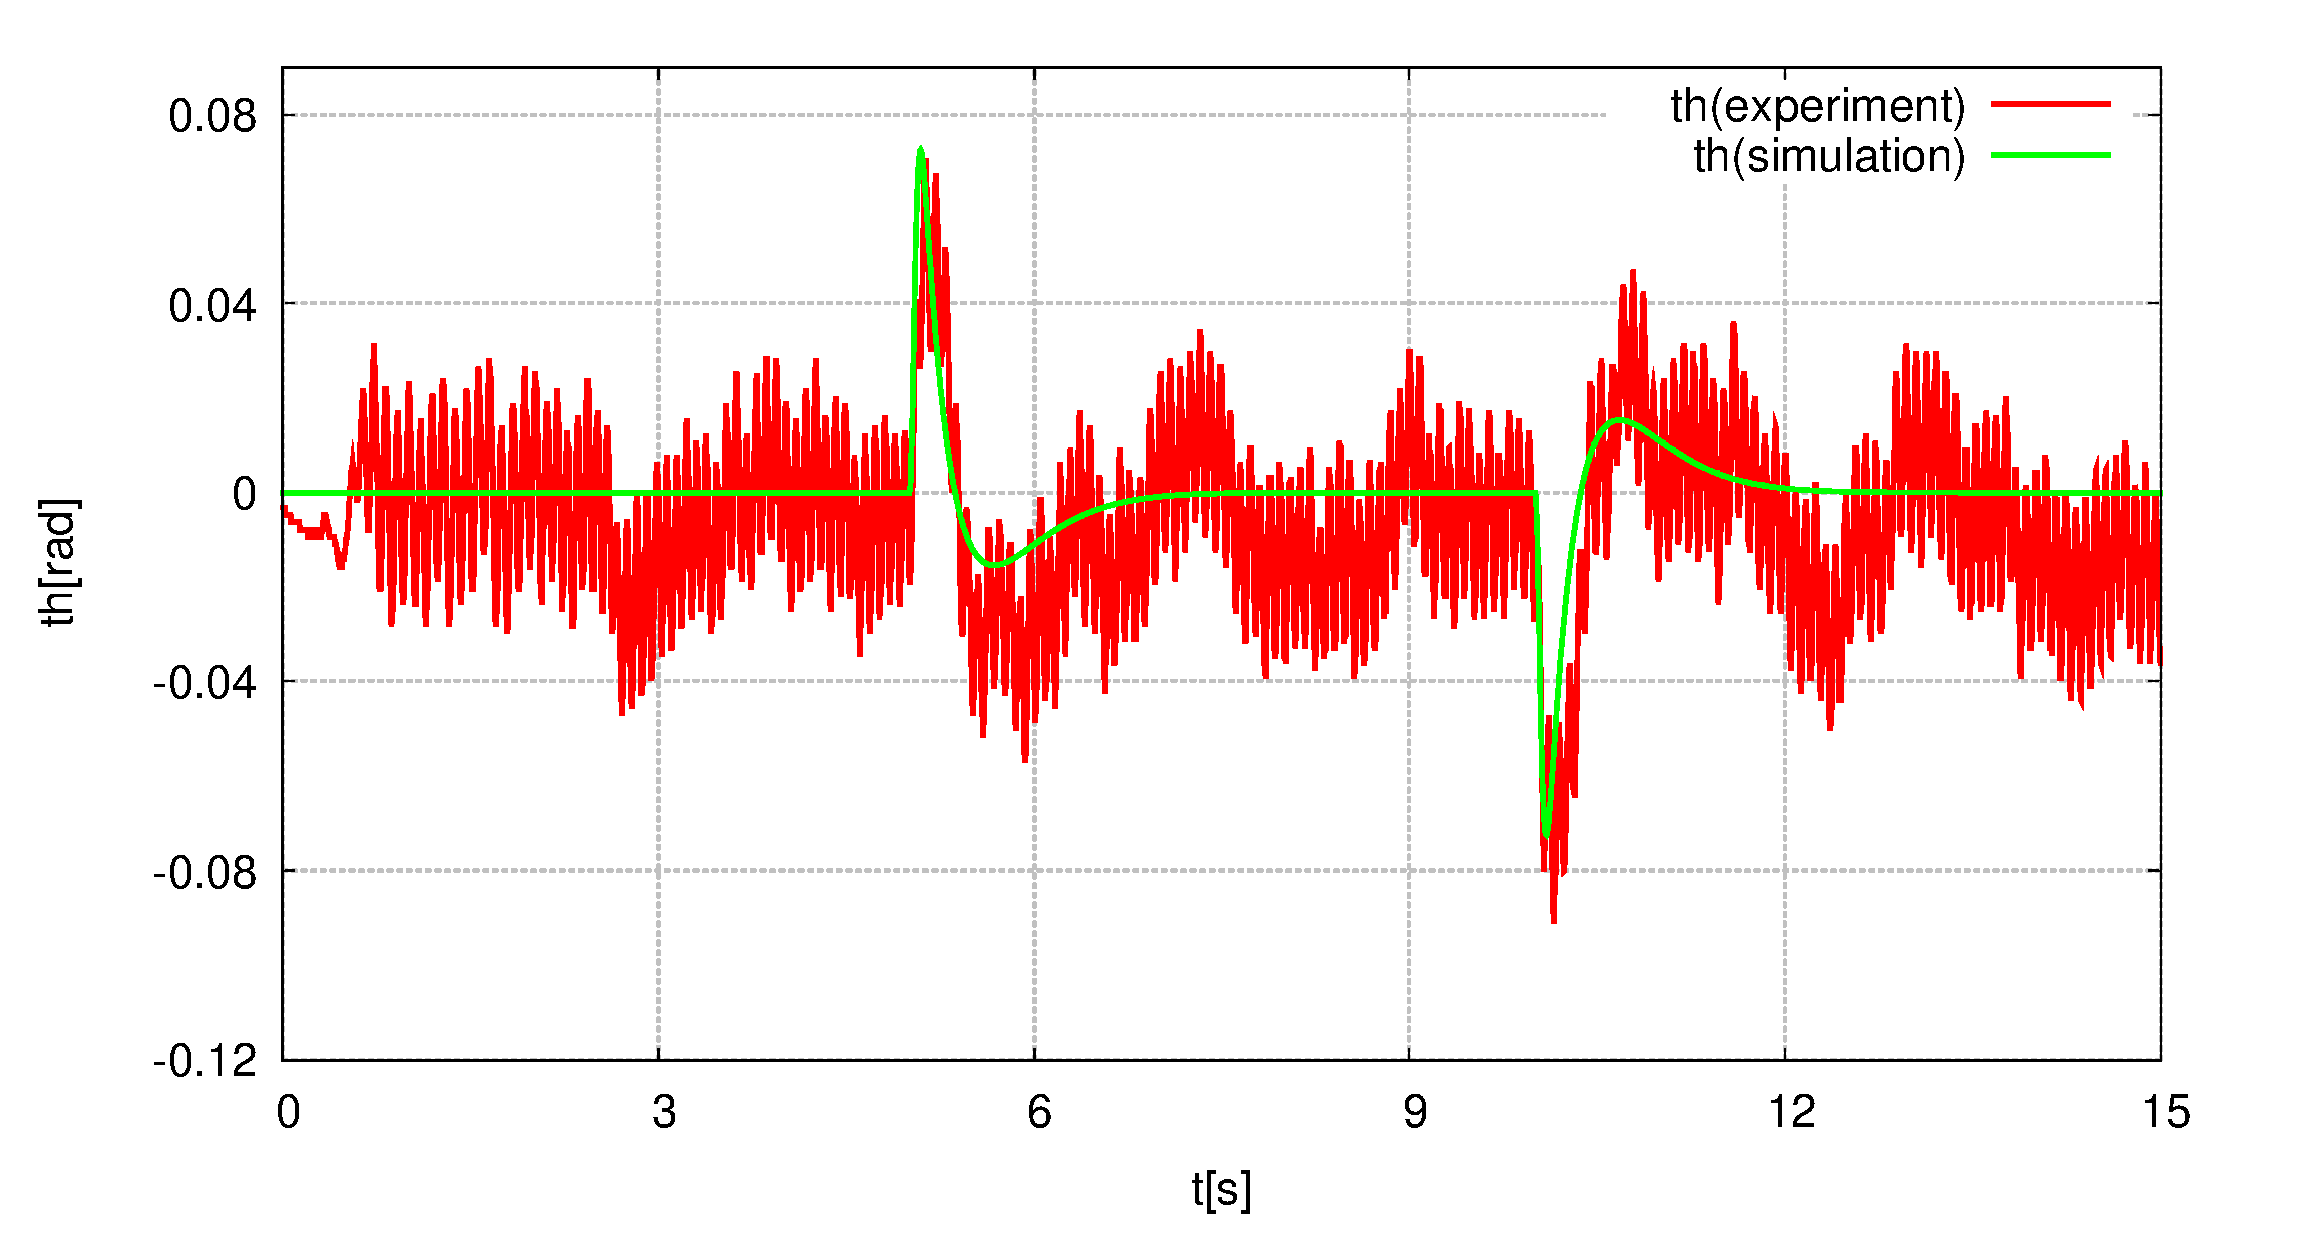
\includegraphics[width=0.49\linewidth]{gazo/experiment_Q55obs60dt05TH2.eps}
		\caption{比較結果その4(左図がr,右図が$\theta$)}
		\label{image:sono4}
	\end{figure}
	\begin{figure}[H]
		\centering
		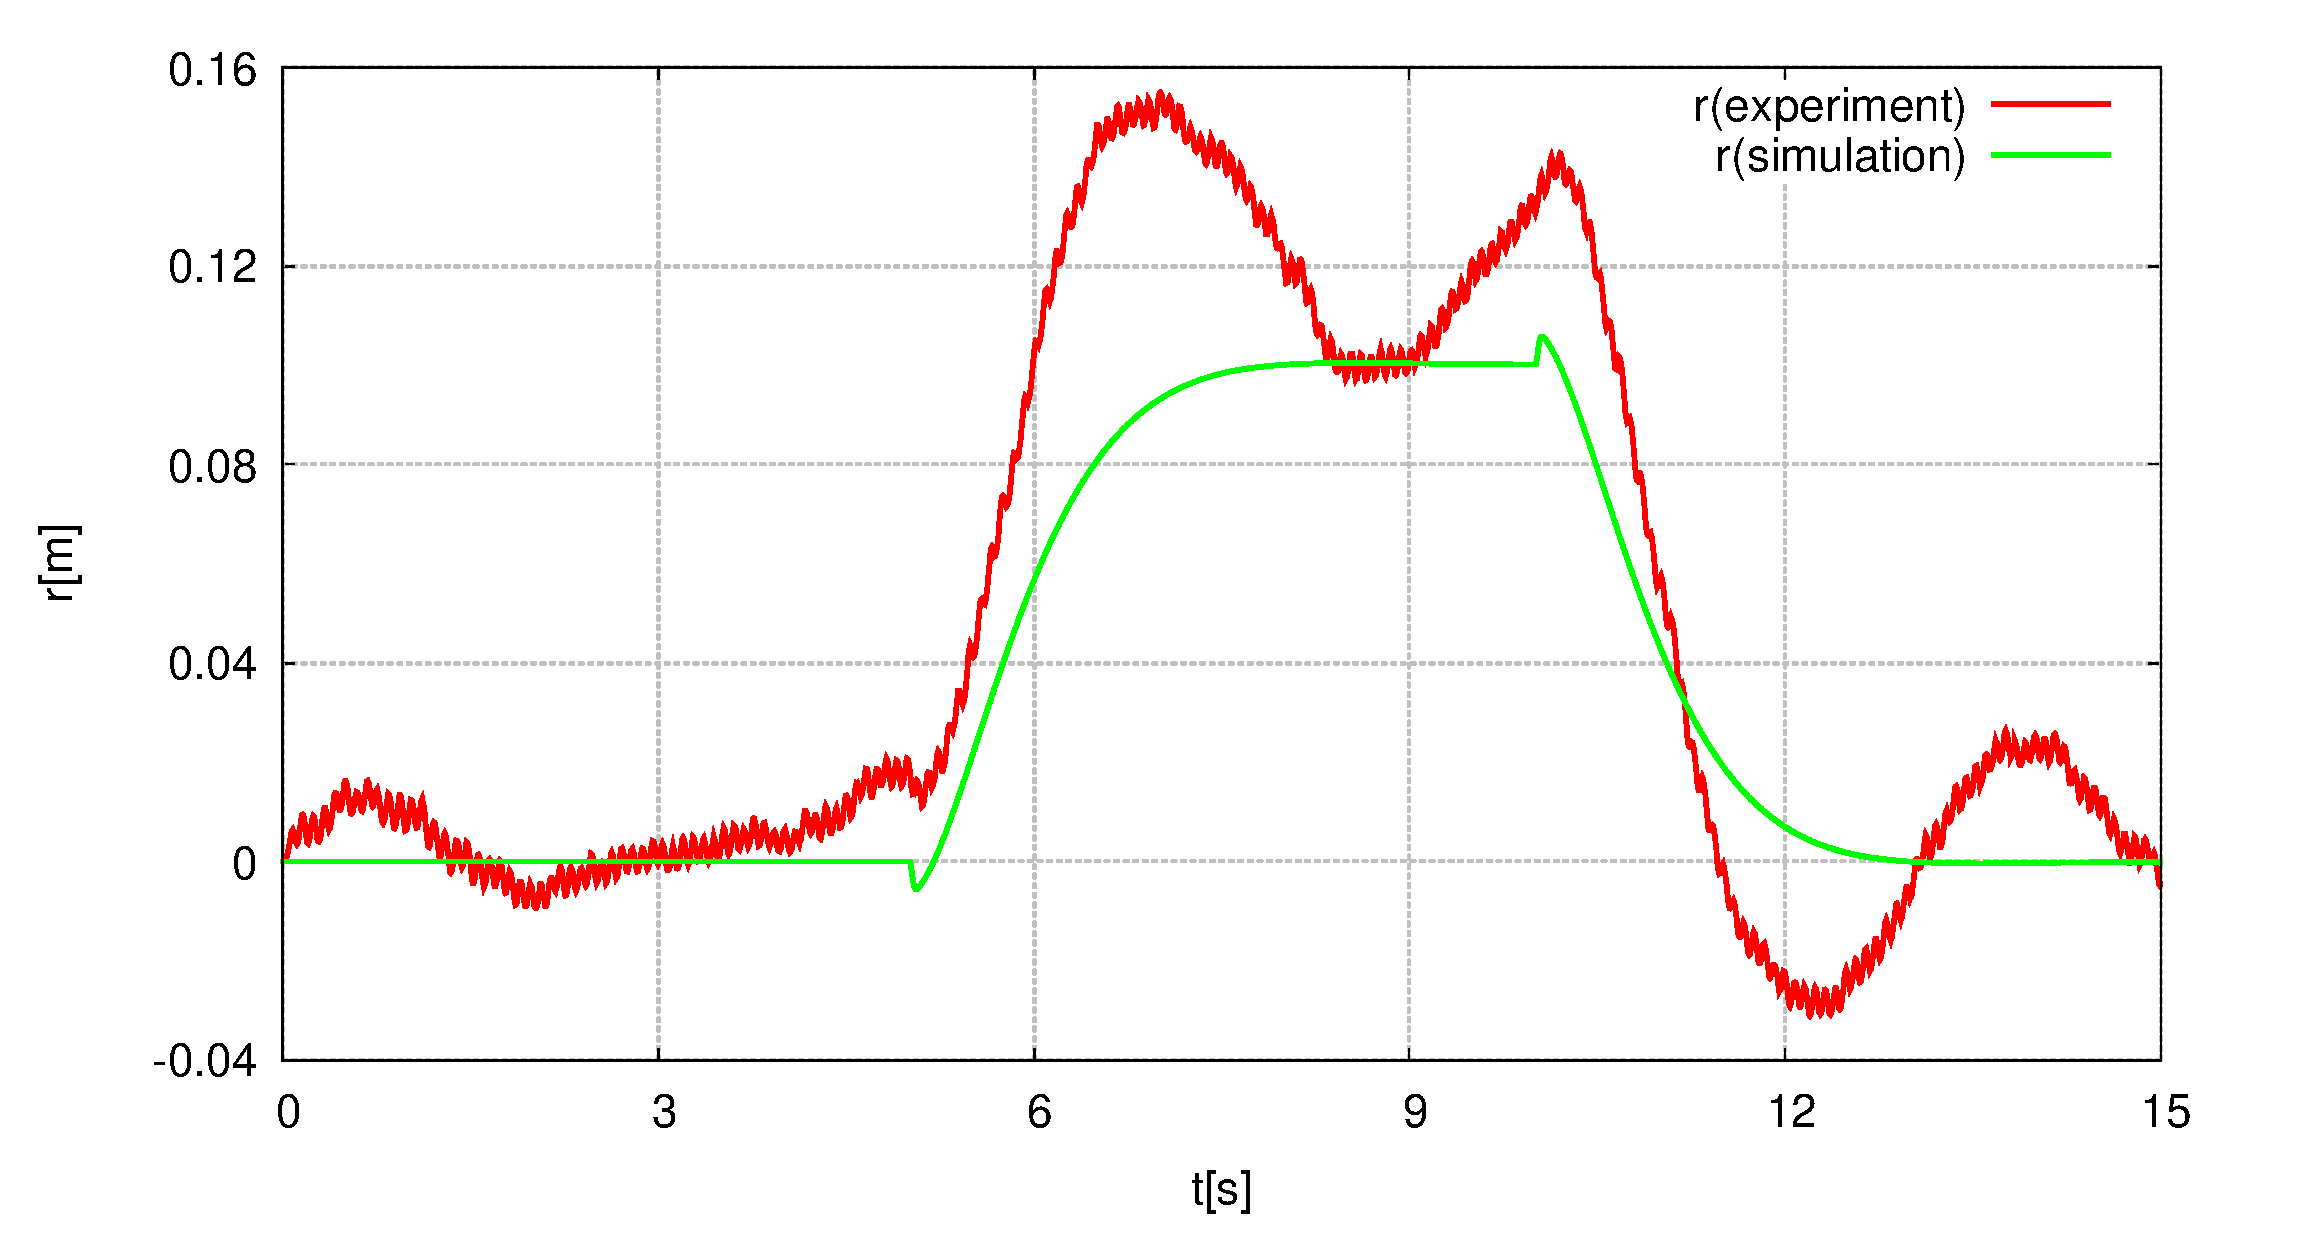
\includegraphics[width=0.49\linewidth]{gazo/experiment_Q56obs60dt05R2.eps}
		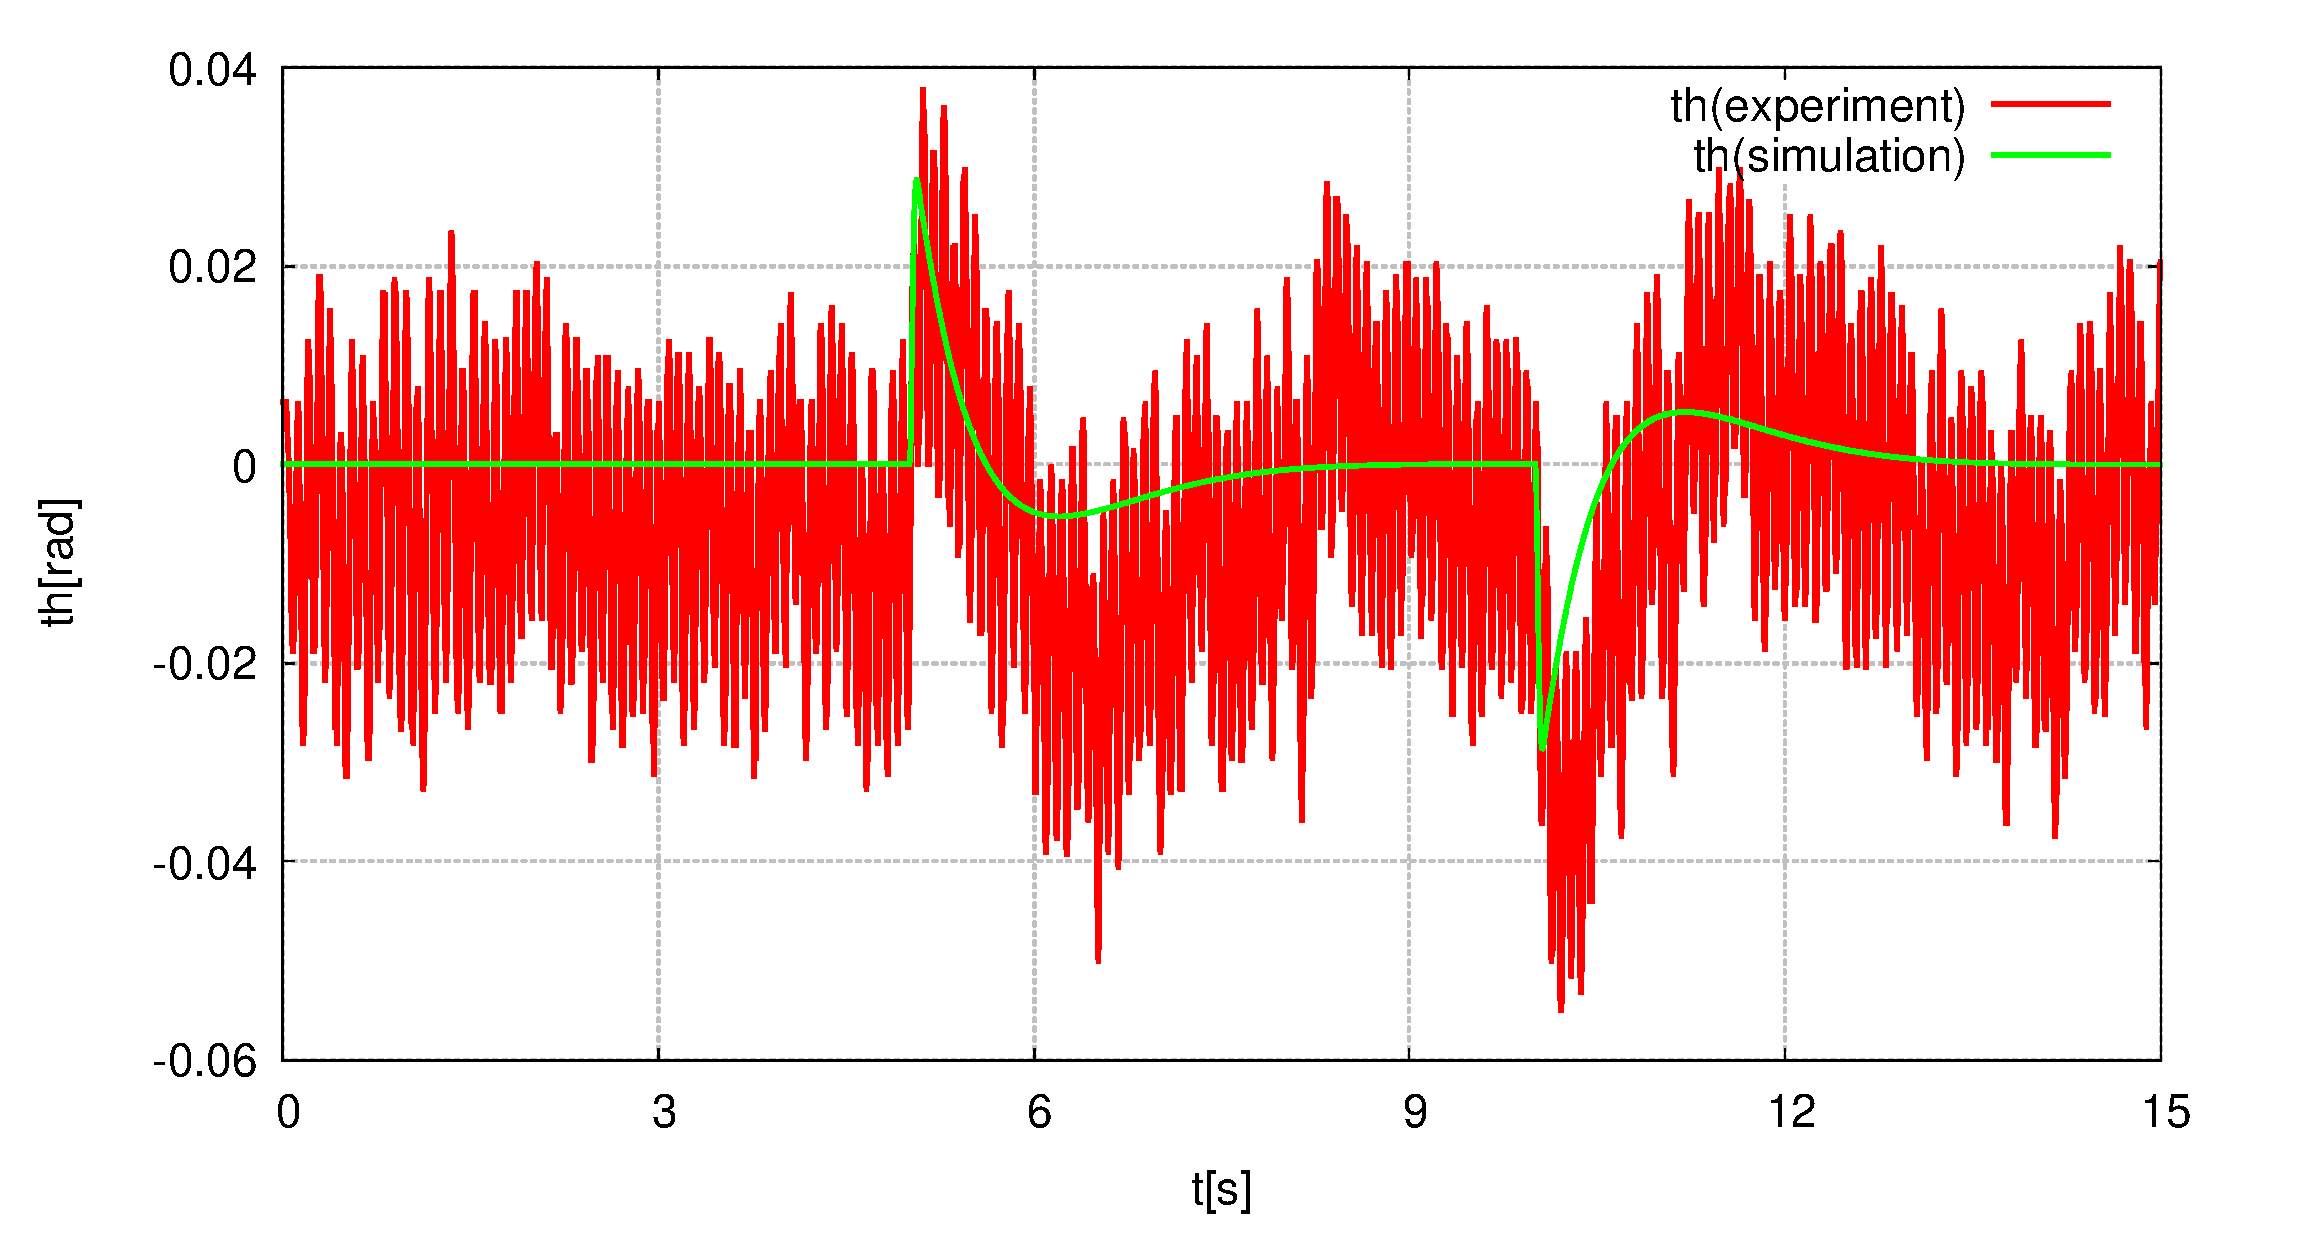
\includegraphics[width=0.49\linewidth]{gazo/experiment_Q56obs60dt05TH2.eps}
		\caption{比較結果その5(左図がr,右図が$\theta$)}
		\label{image:sono5}
	\end{figure}
	\begin{figure}[H]
		\centering
		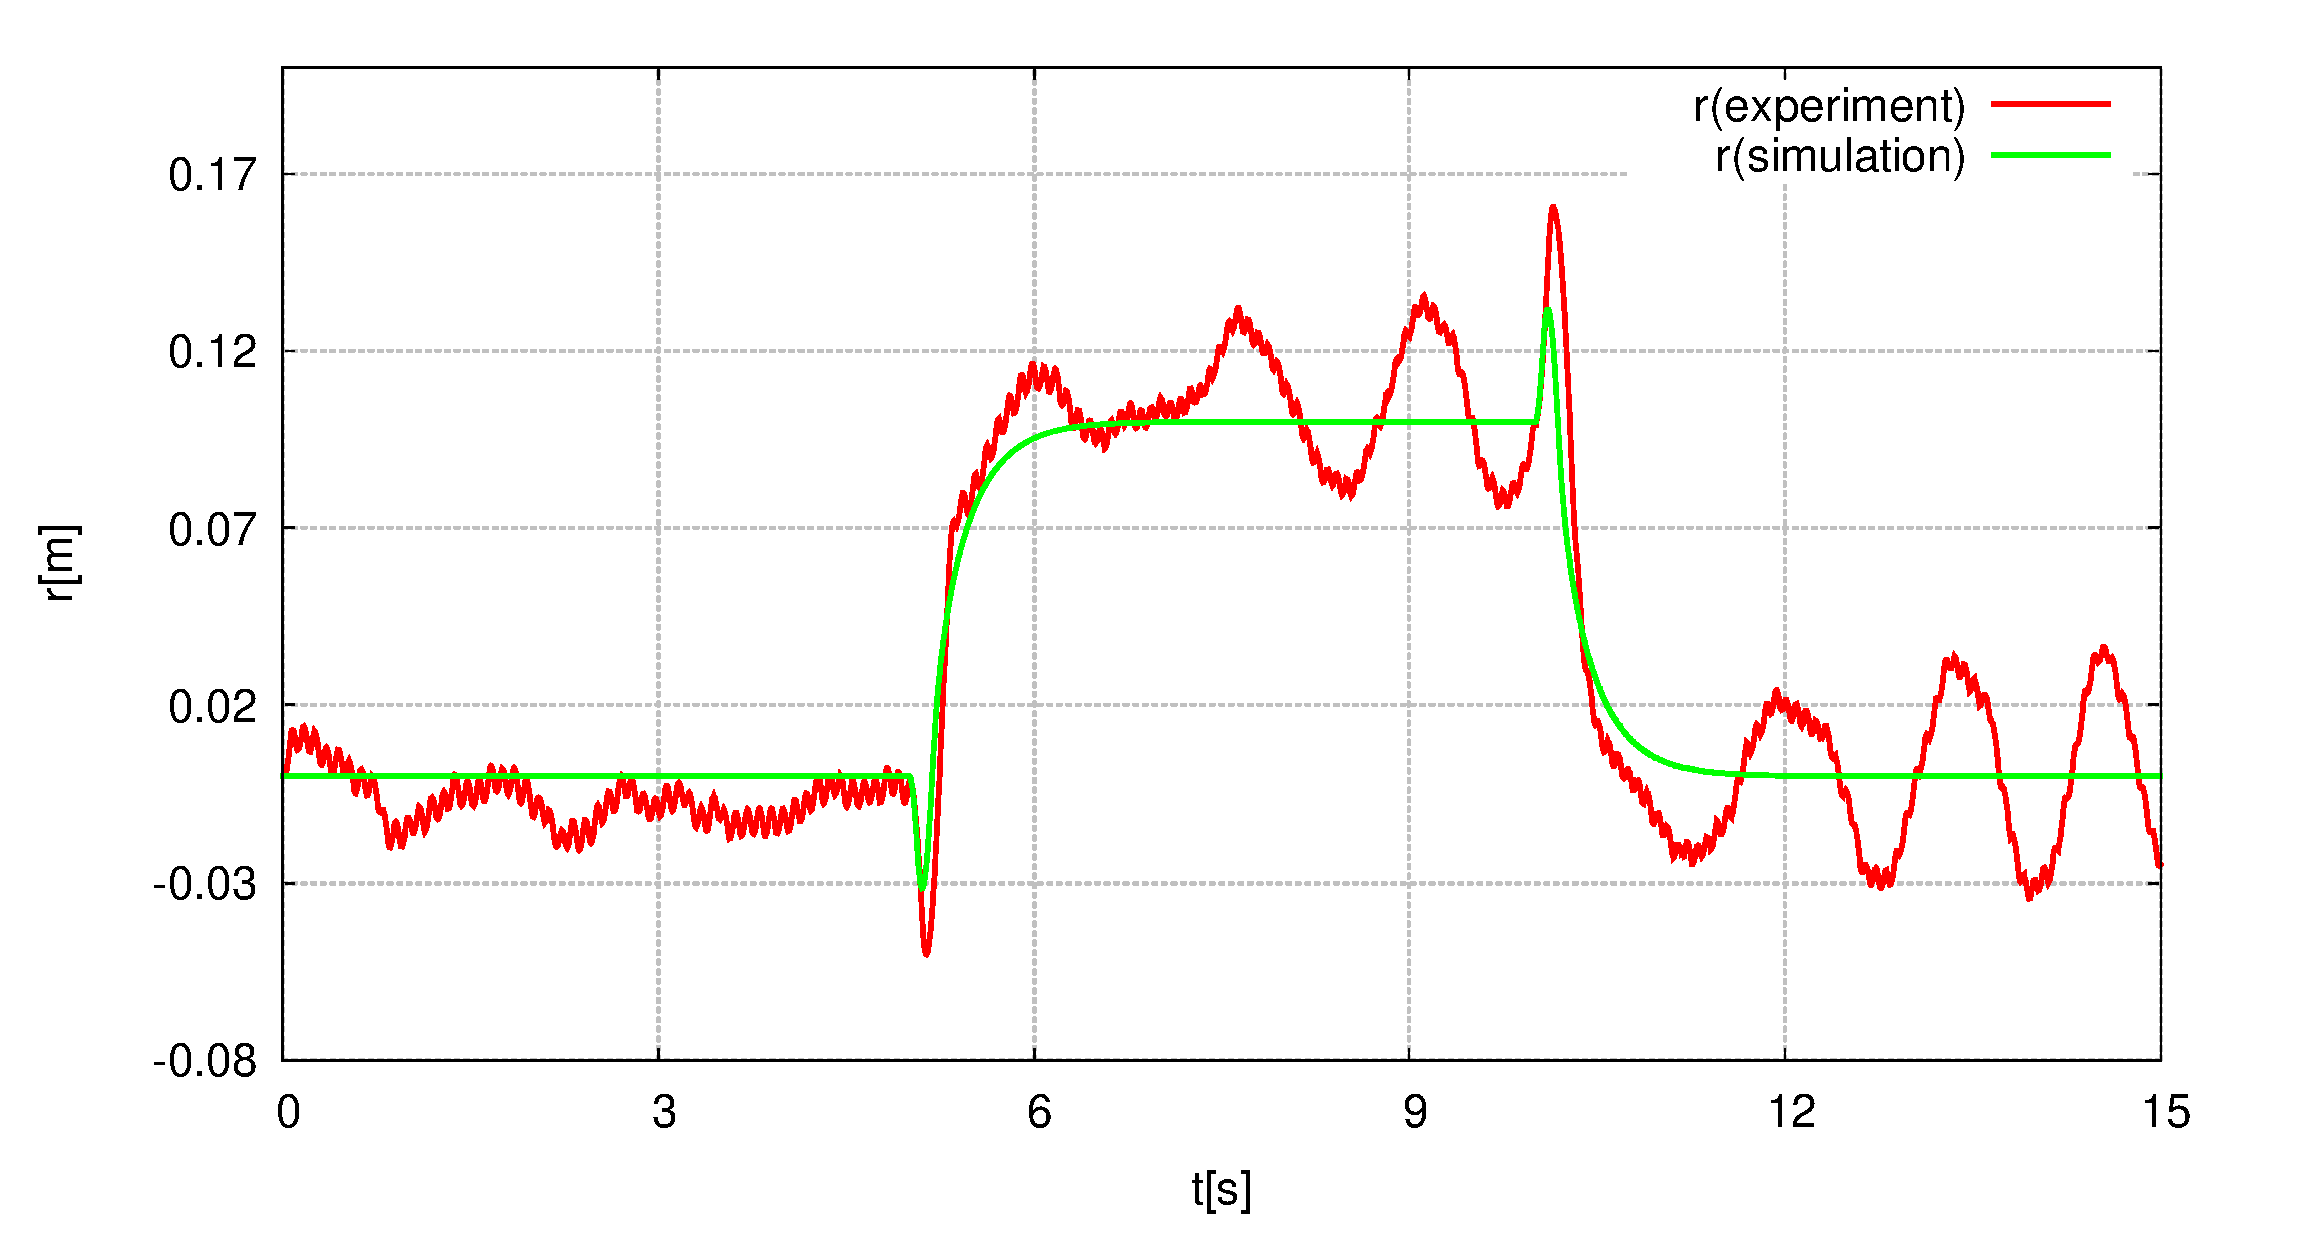
\includegraphics[width=0.49\linewidth]{gazo/experiment_Q65obs60dt05R2.eps}
		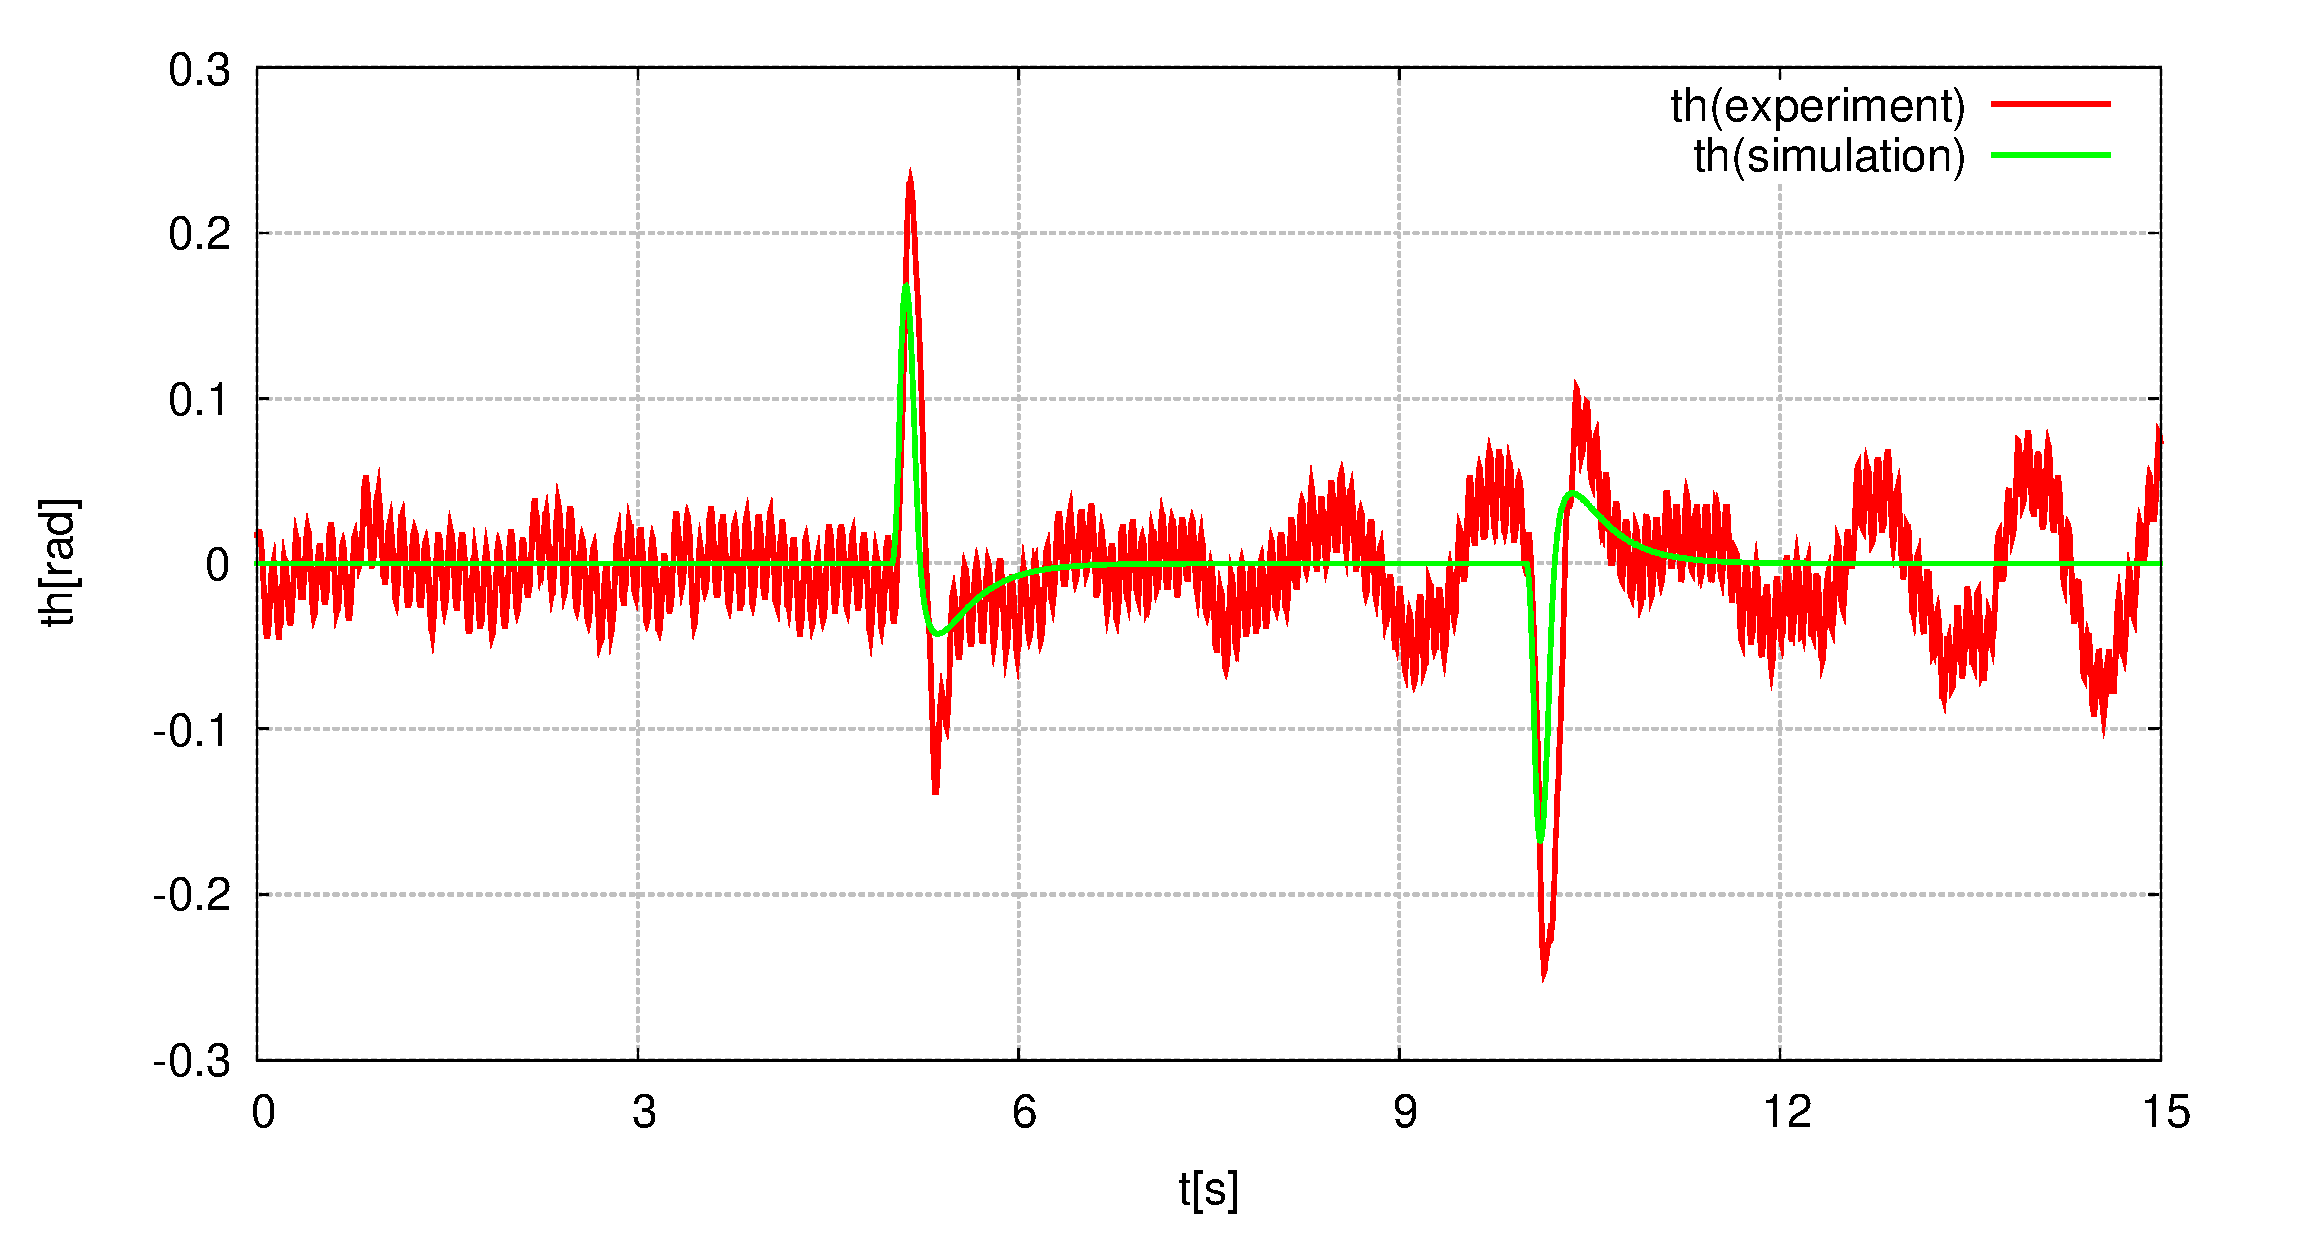
\includegraphics[width=0.49\linewidth]{gazo/experiment_Q65obs60dt05TH2.eps}
		\caption{比較結果その6(左図がr,右図が$\theta$)}
		\label{image:sono6}
	\end{figure}
	\begin{figure}[H]
		\centering
		\includegraphics[width=0.49\linewidth]{gazo/experiment_Q55obs30dt10R2.eps}
		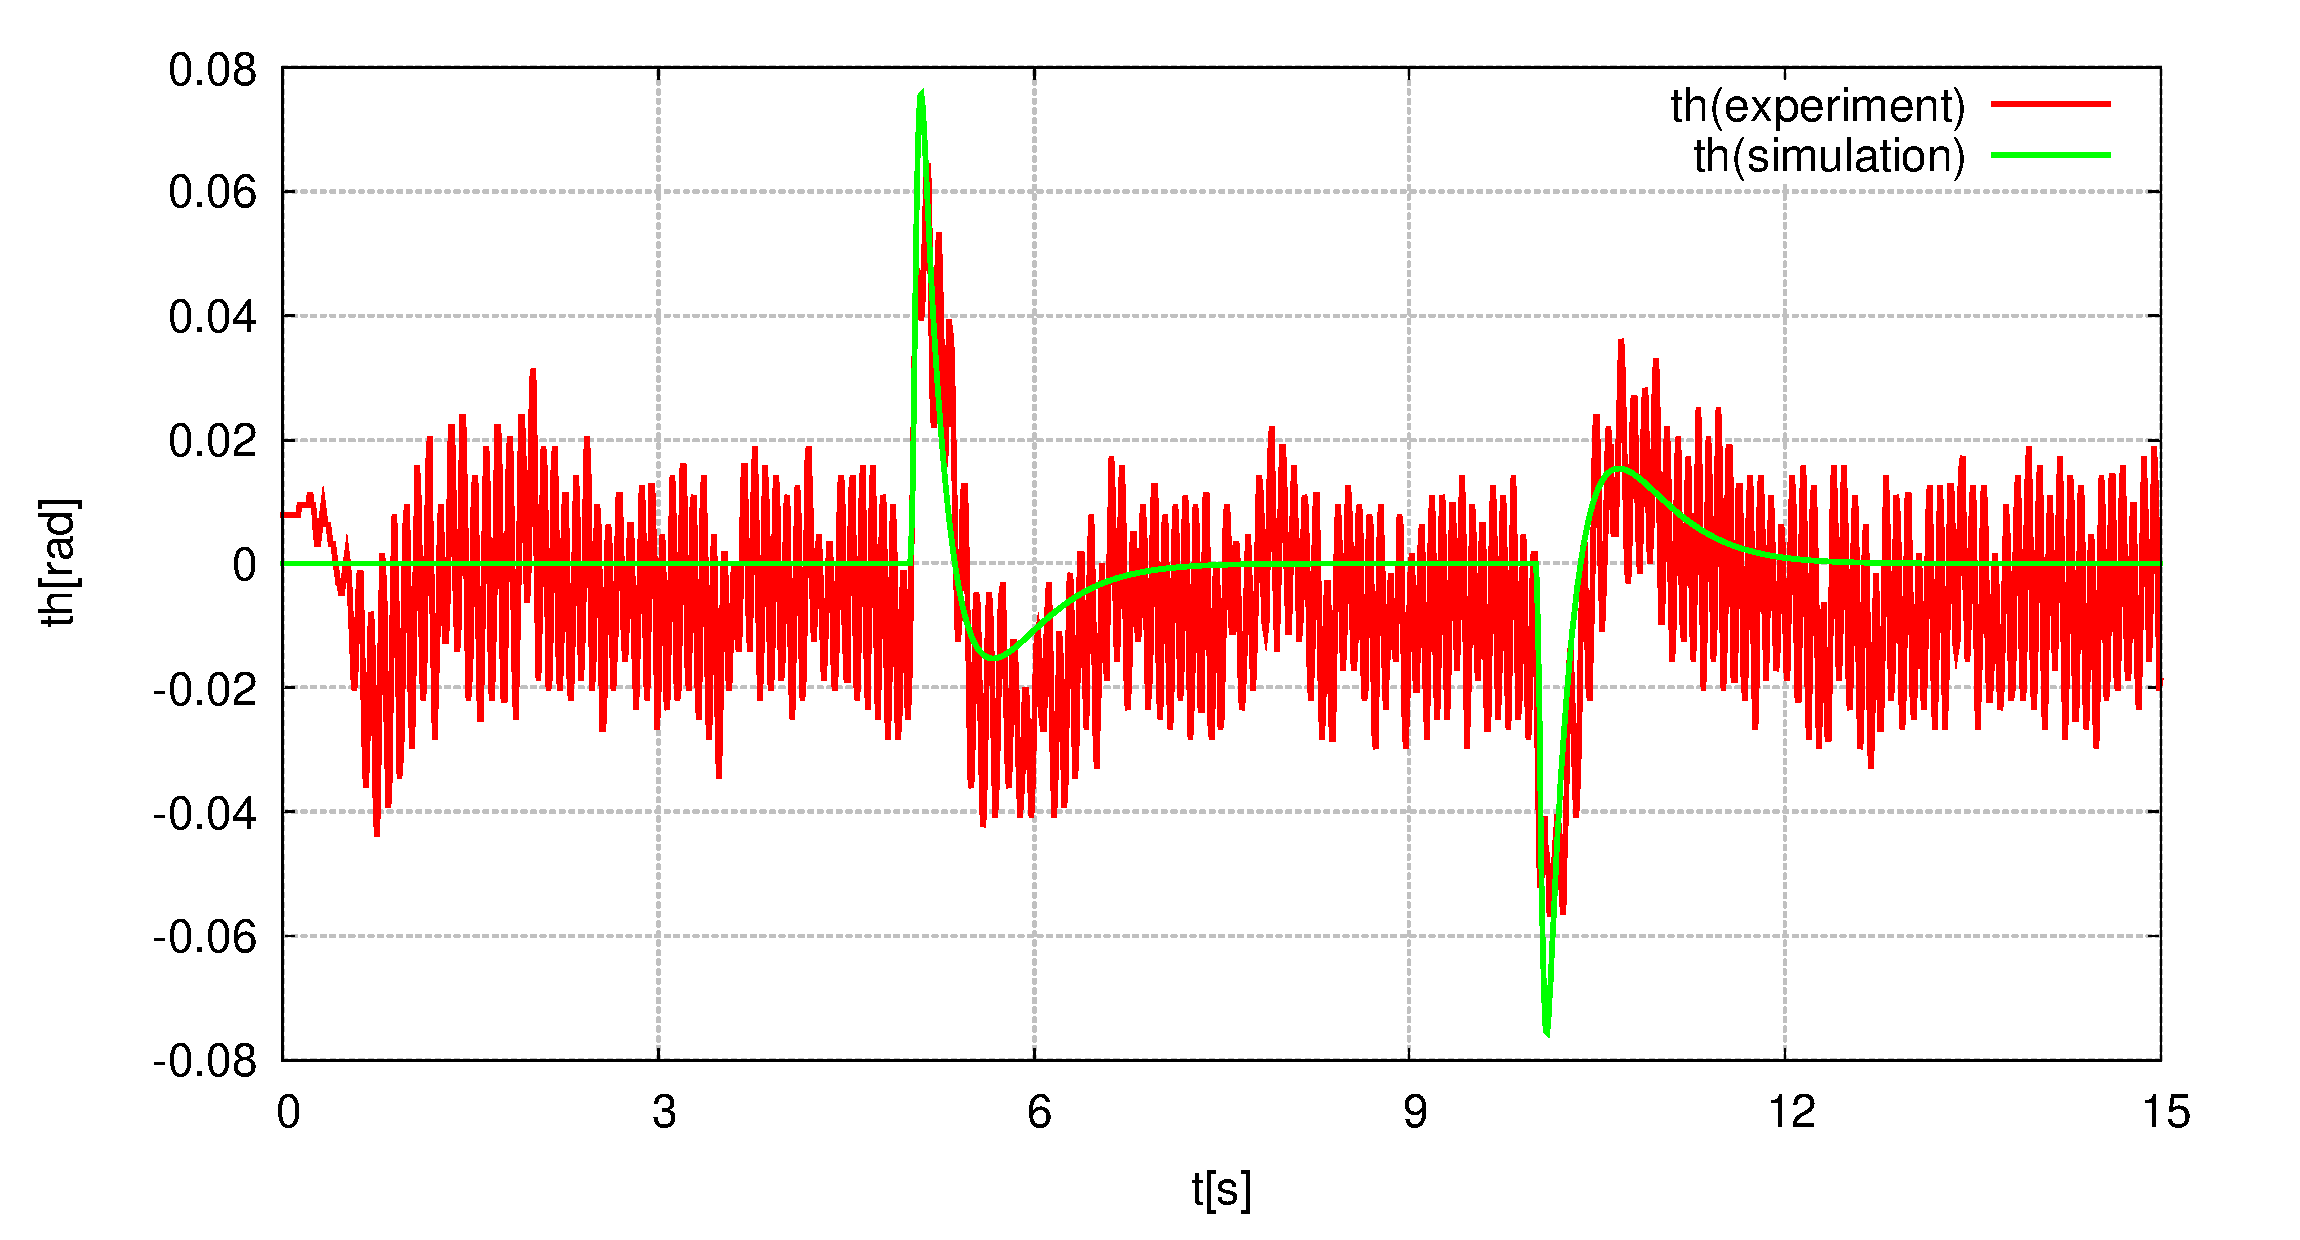
\includegraphics[width=0.49\linewidth]{gazo/experiment_Q55obs30dt10TH2.eps}
		\caption{比較結果その7(左図がr,右図が$\theta$)}
		\label{image:sono7}
	\end{figure}
	\begin{figure}[H]
		\centering
		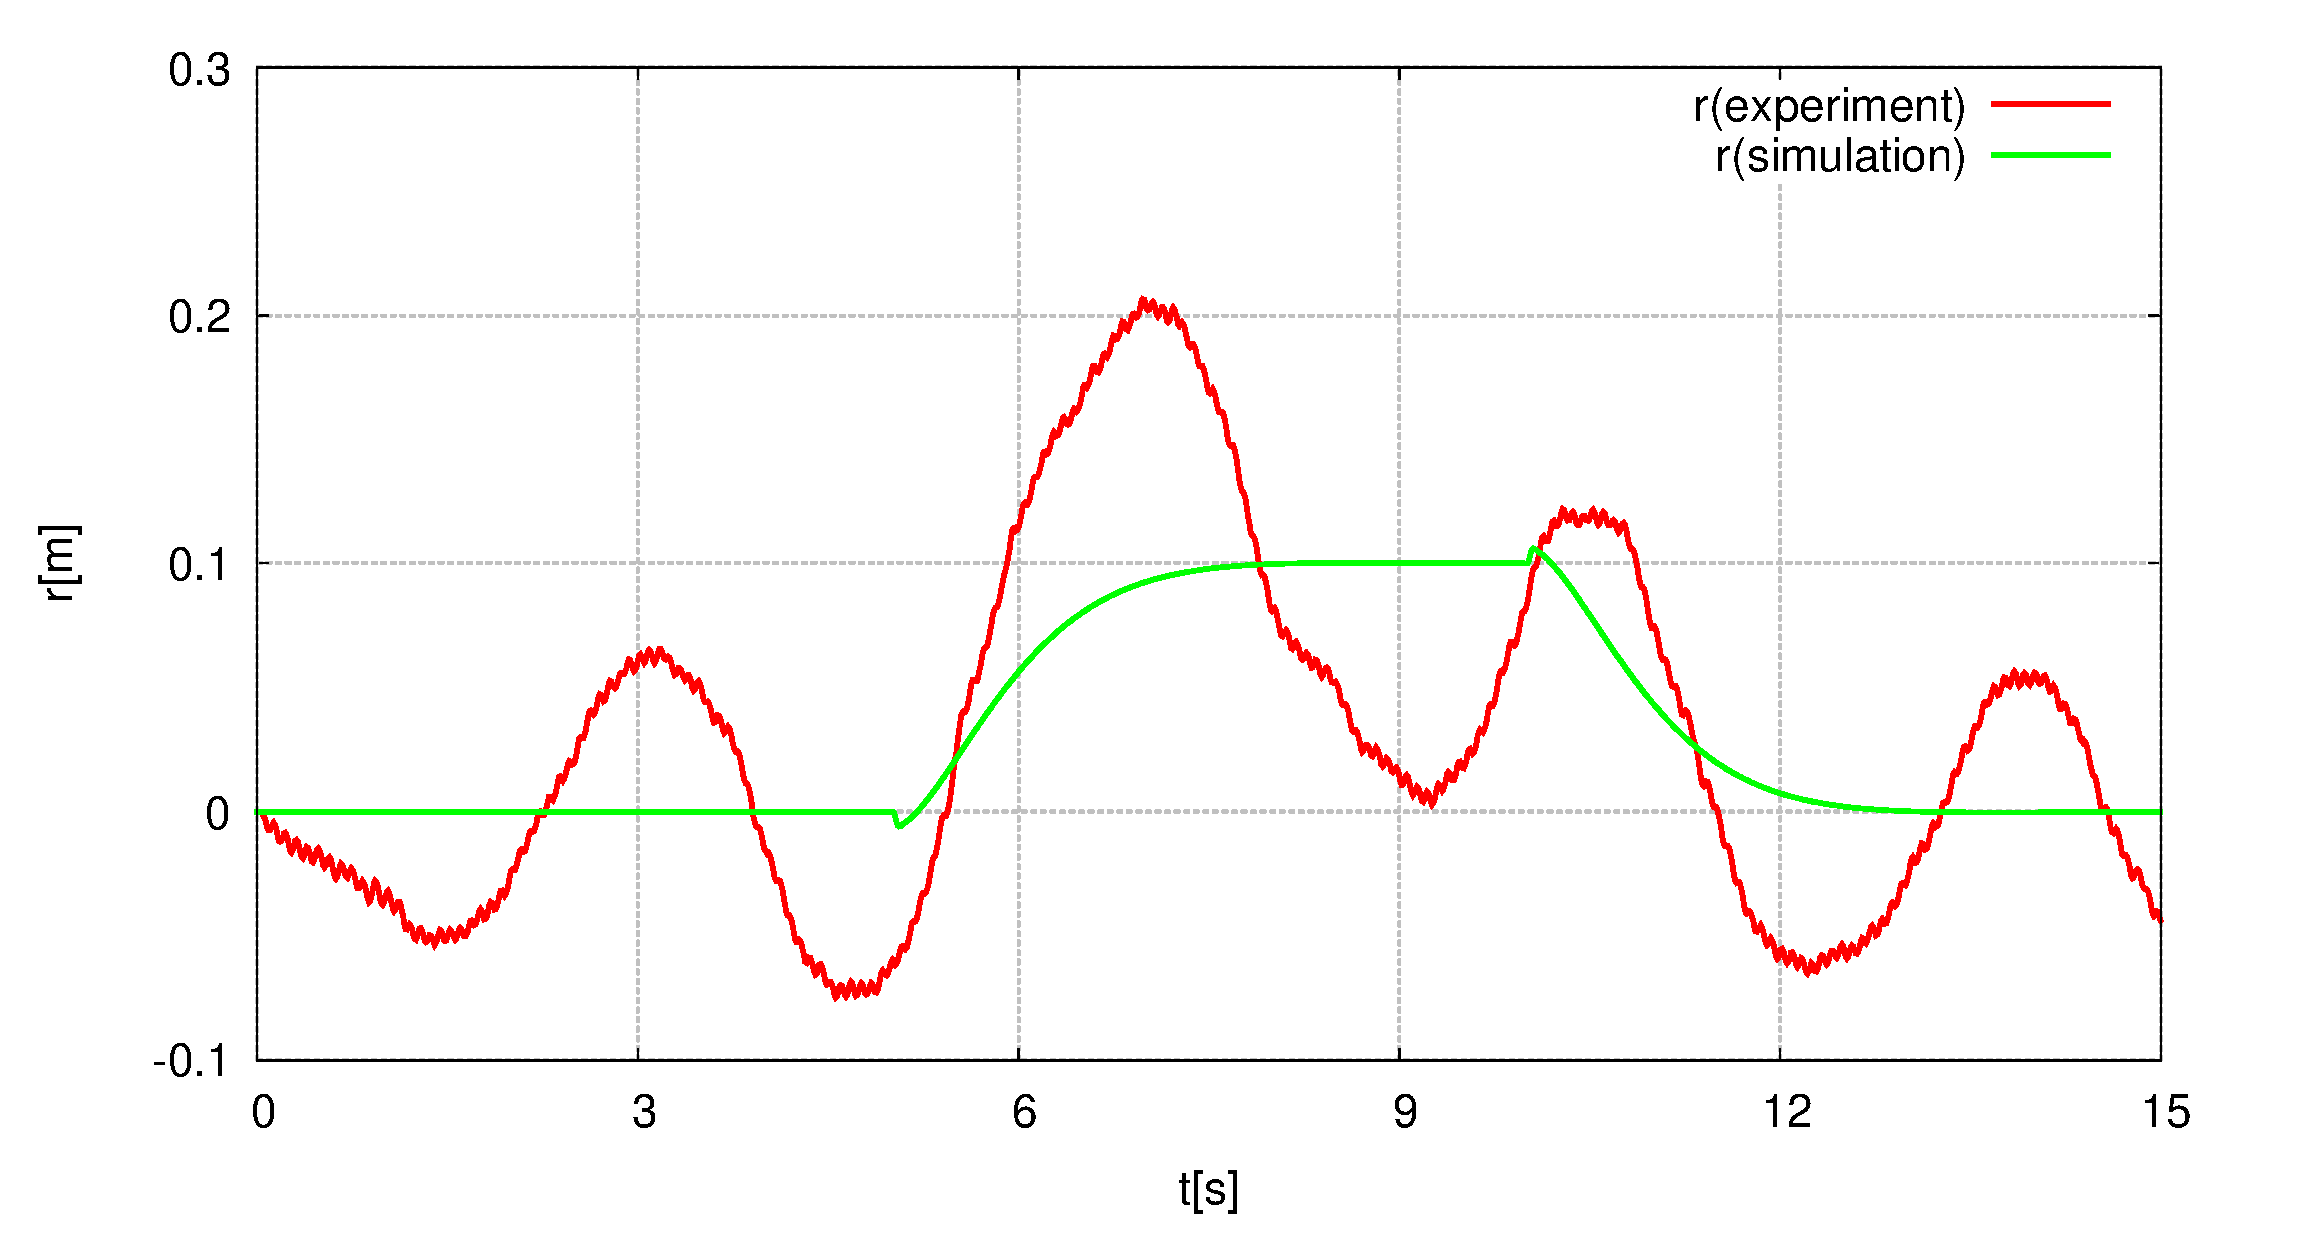
\includegraphics[width=0.49\linewidth]{gazo/experiment_Q56obs30dt10R2.eps}
		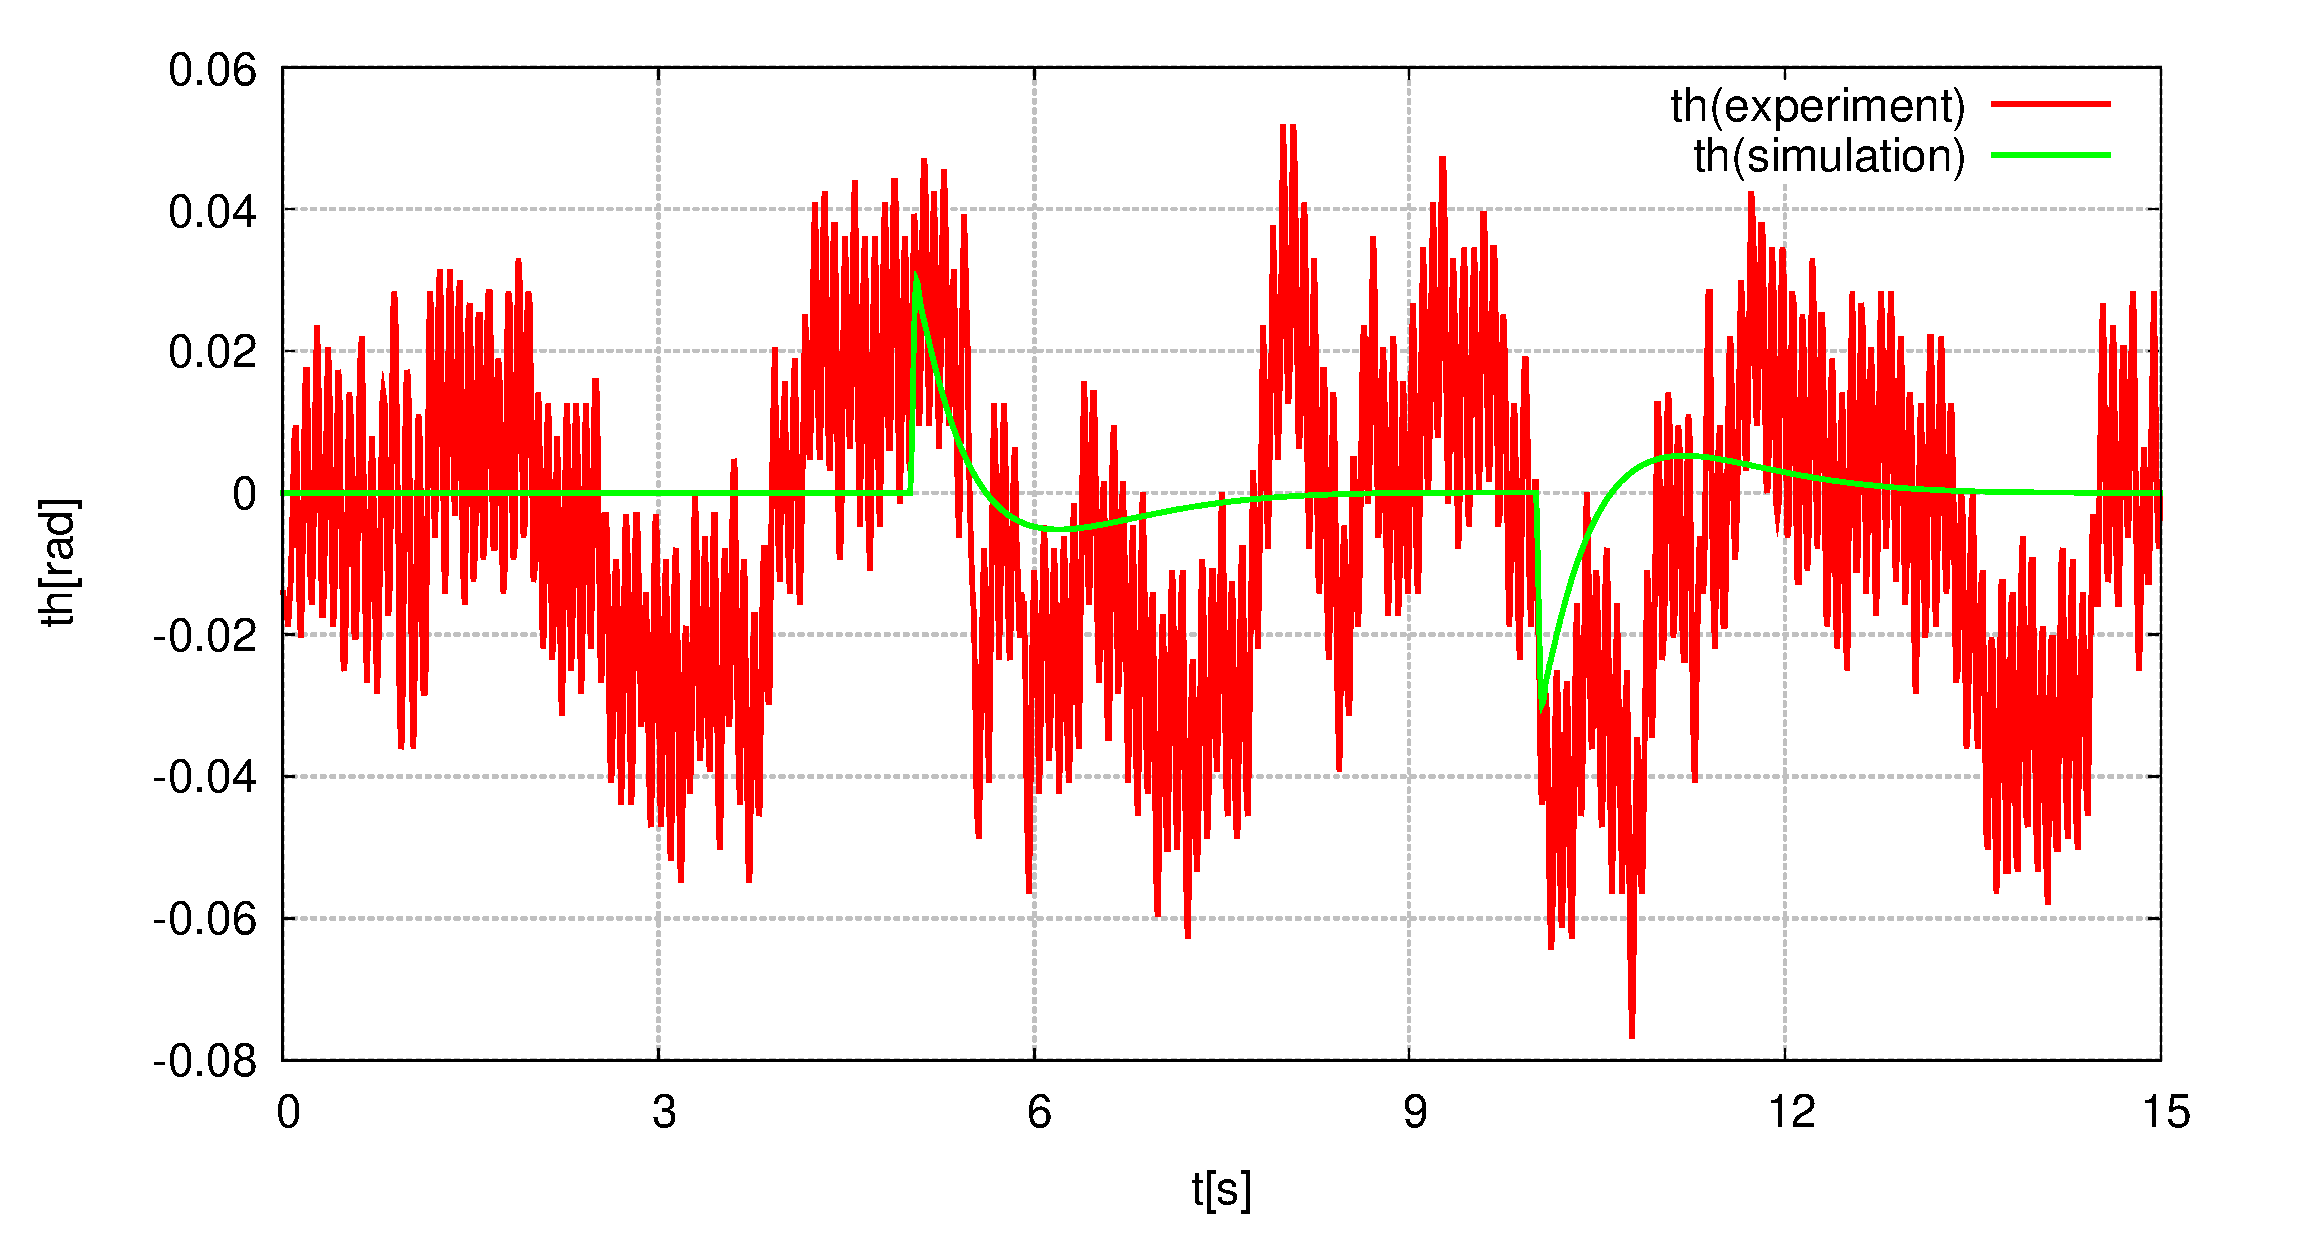
\includegraphics[width=0.49\linewidth]{gazo/experiment_Q56obs30dt10TH2.eps}
		\caption{比較結果その8(左図がr,右図が$\theta$)}
		\label{image:sono8}
	\end{figure}
	\begin{figure}[H]
		\centering
		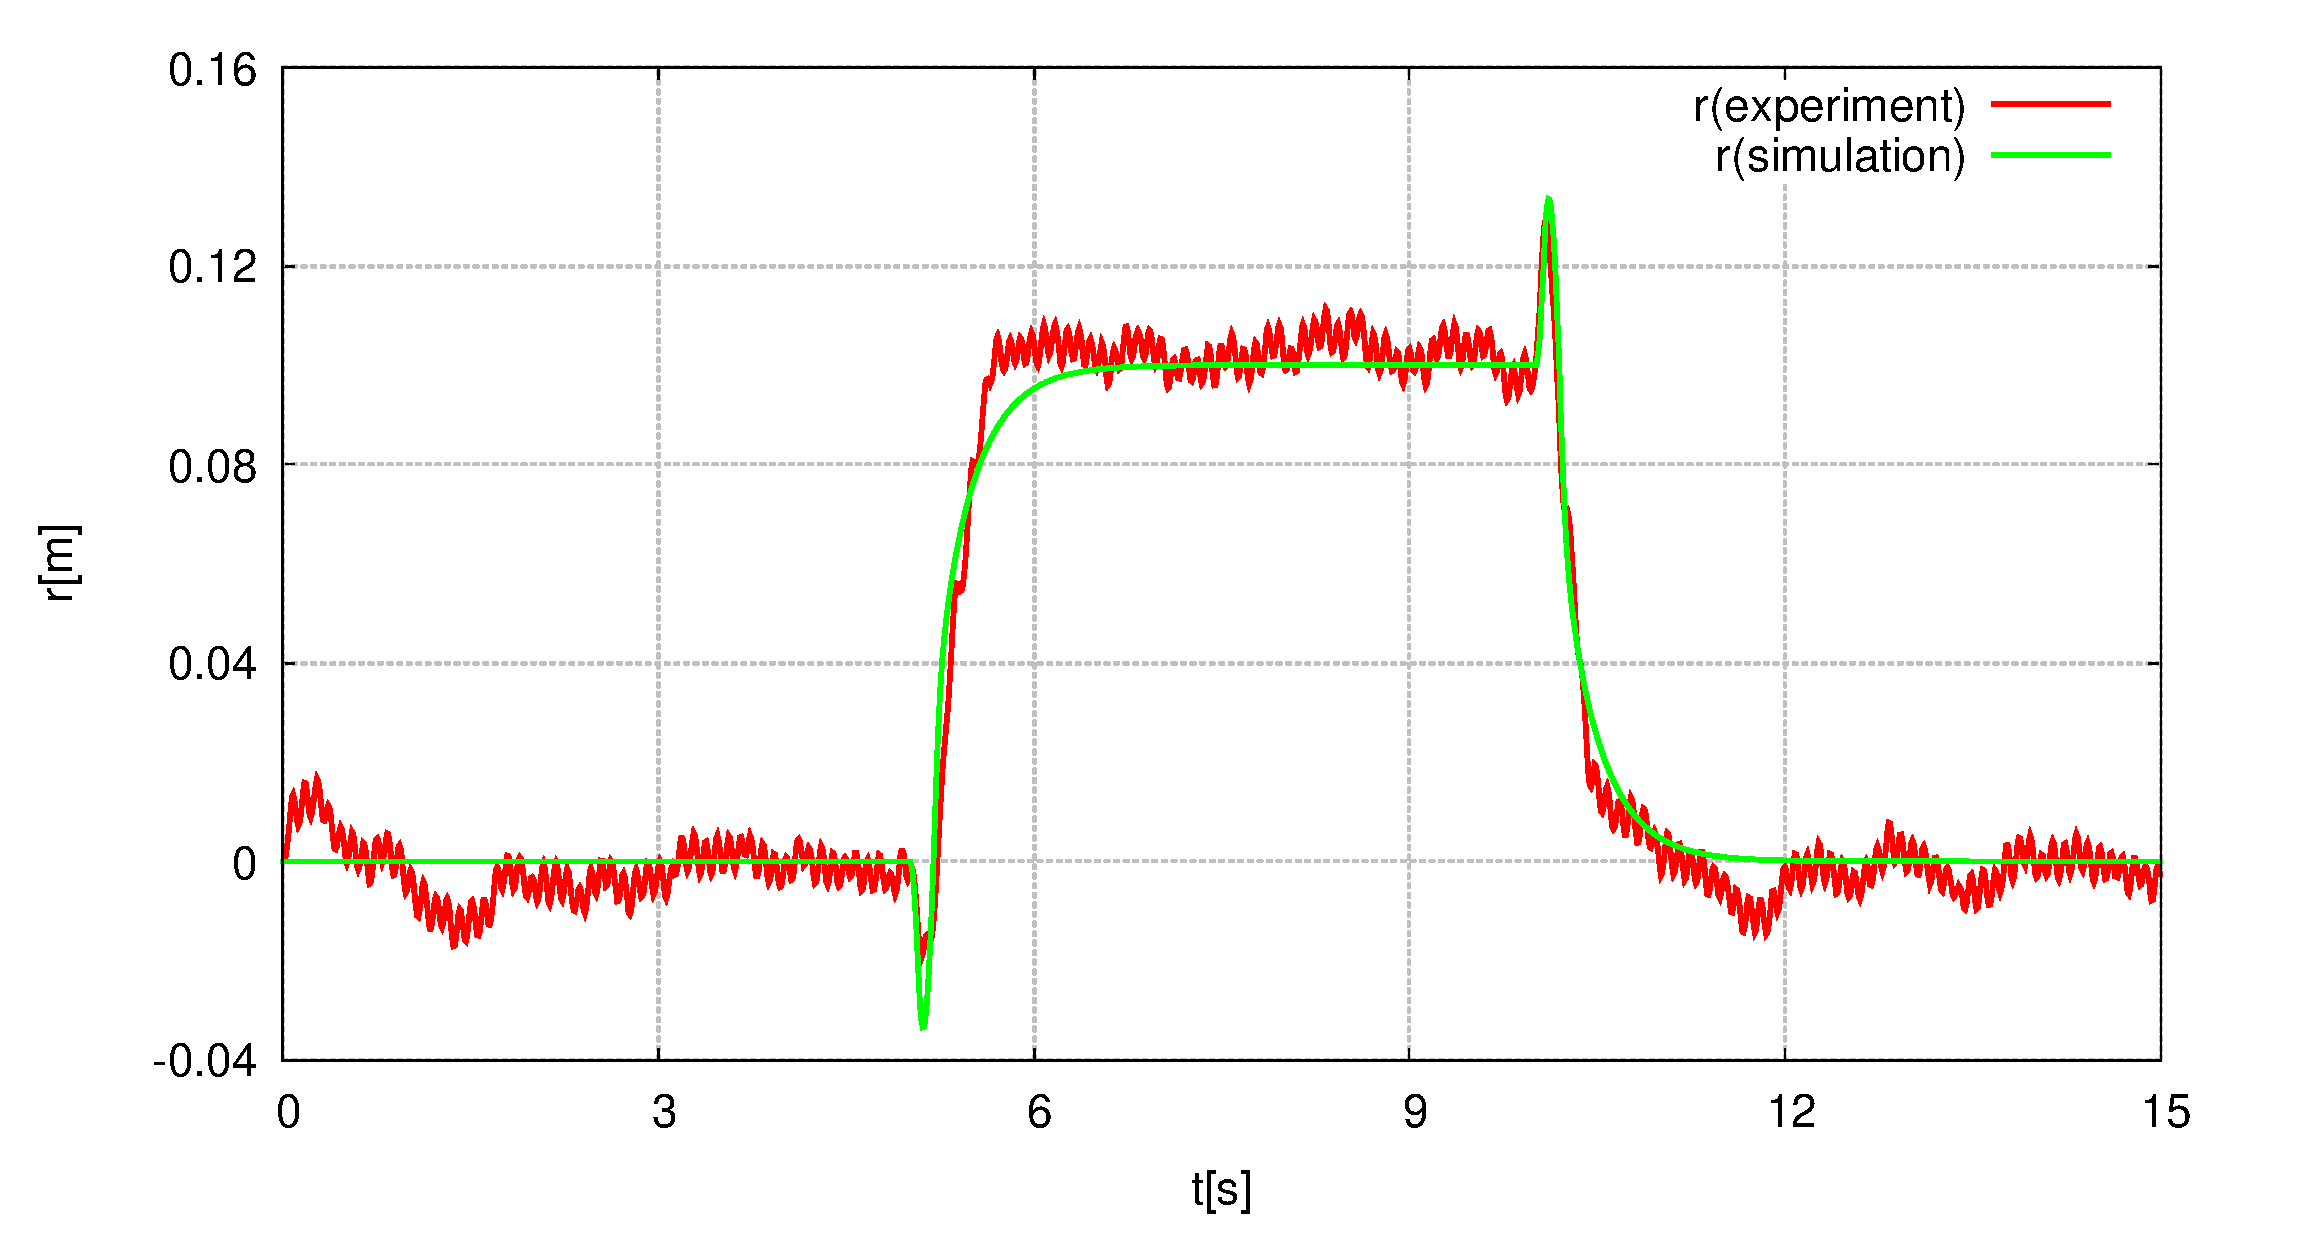
\includegraphics[width=0.49\linewidth]{gazo/experiment_Q65obs30dt10R2.eps}
		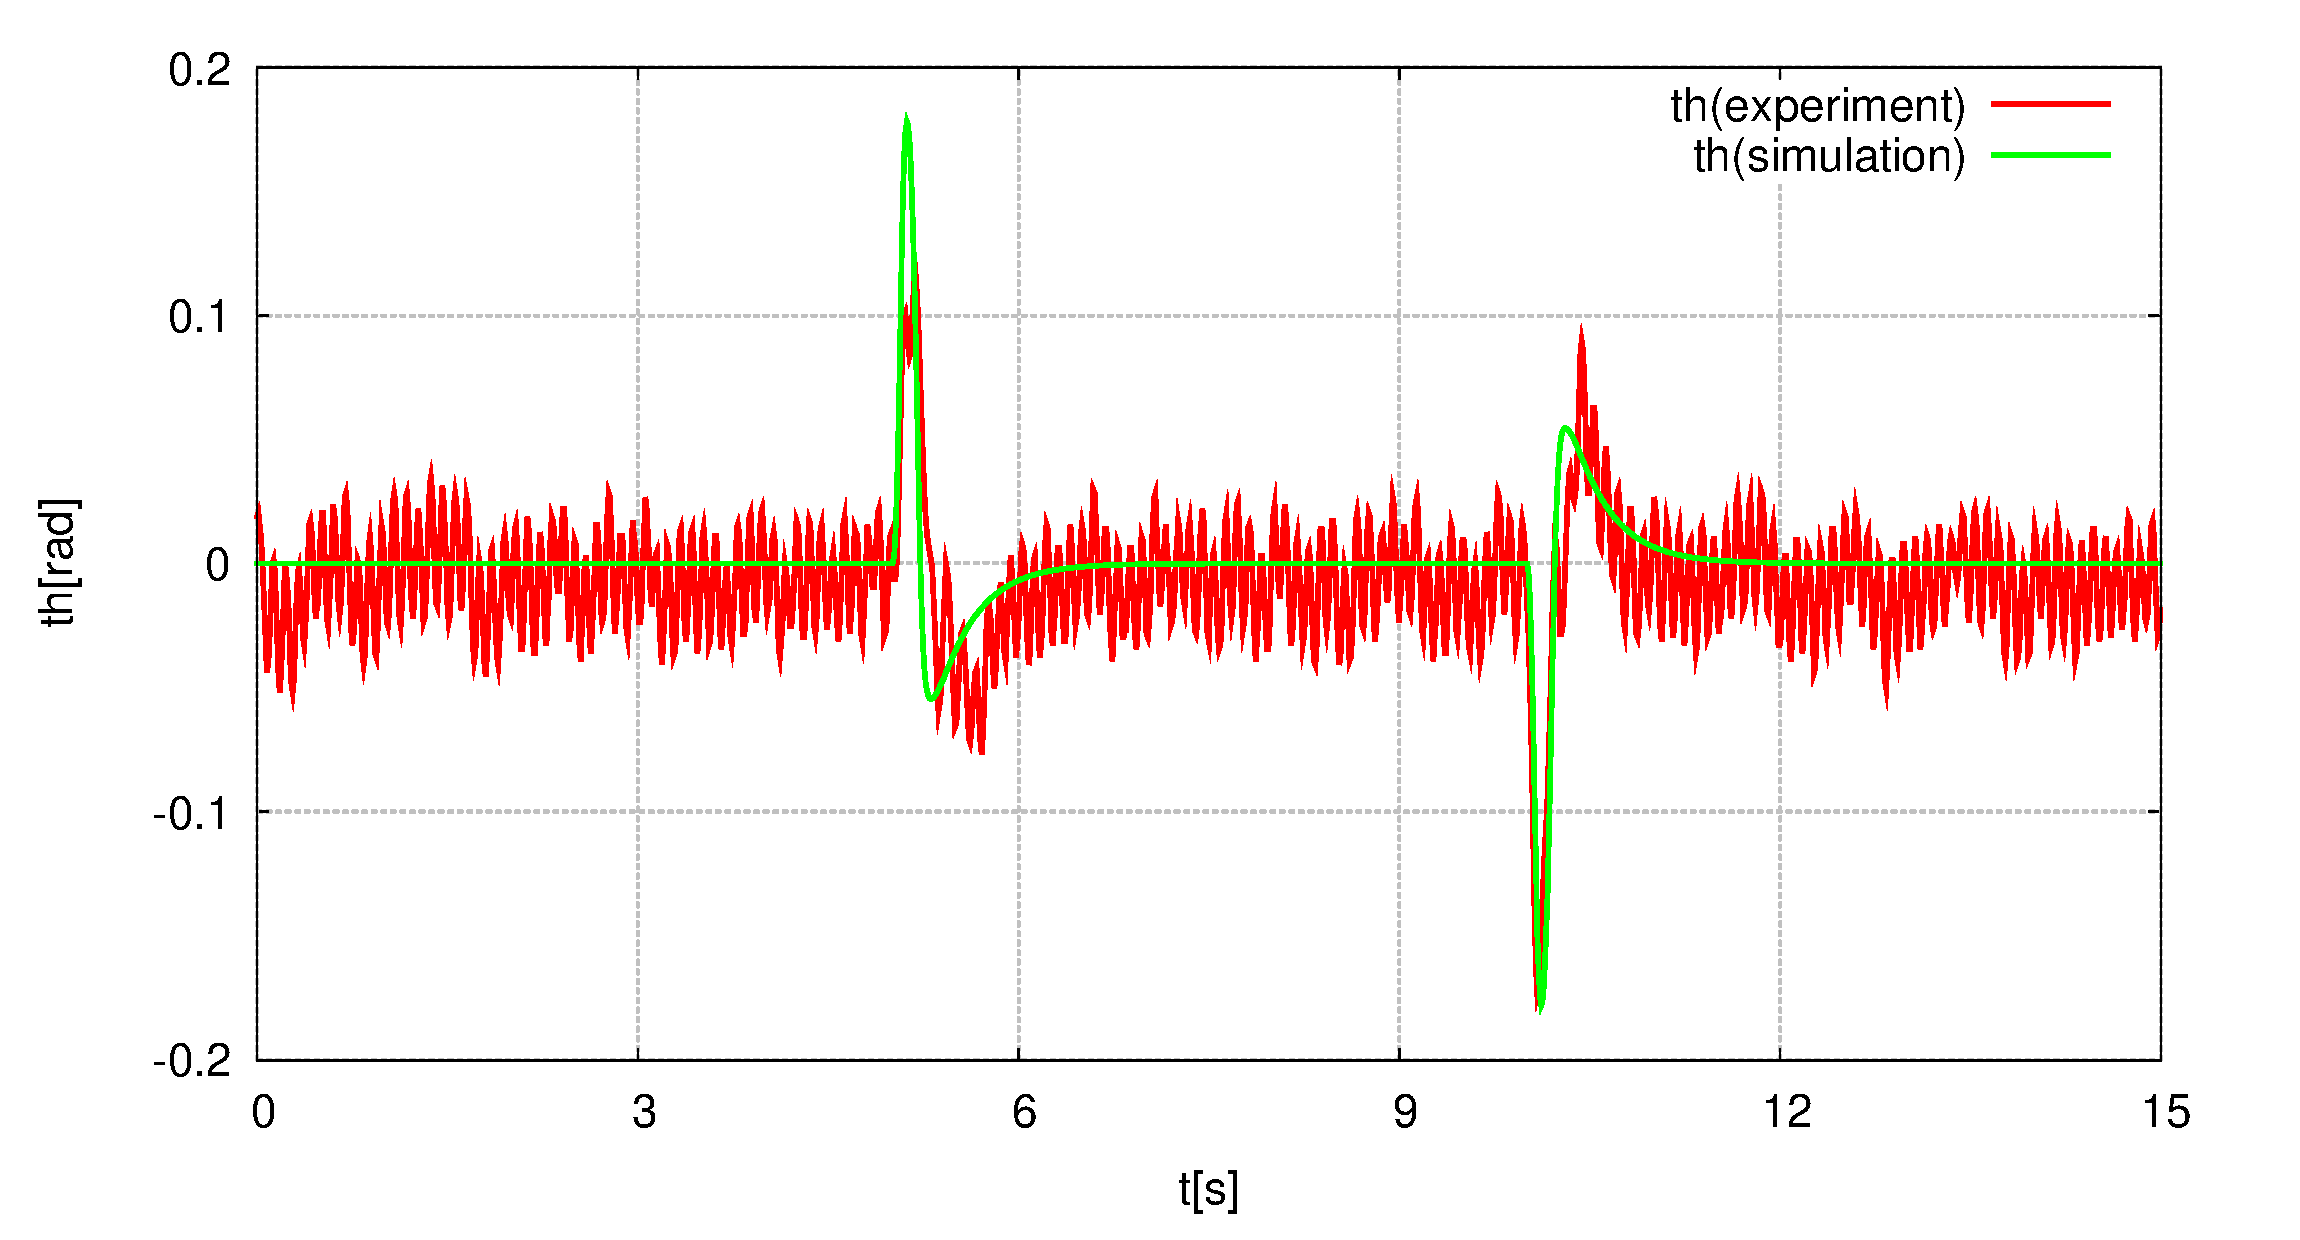
\includegraphics[width=0.49\linewidth]{gazo/experiment_Q65obs30dt10TH2.eps}
		\caption{比較結果その9(左図がr,右図が$\theta$)}
		\label{image:sono9}
	\end{figure}
	\begin{figure}[H]
		\centering
		\includegraphics[width=0.49\linewidth]{gazo/experiment_Q55obs60dt10R2.eps}
		\includegraphics[width=0.49\linewidth]{gazo/experiment_Q55obs60dt10TH2.eps}
		\caption{比較結果その10(左図がr,右図が$\theta$)}
		\label{image:sono10}
	\end{figure}
	\begin{figure}[H]
		\centering
		\includegraphics[width=0.49\linewidth]{gazo/experiment_Q56obs60dt10R2.eps}
		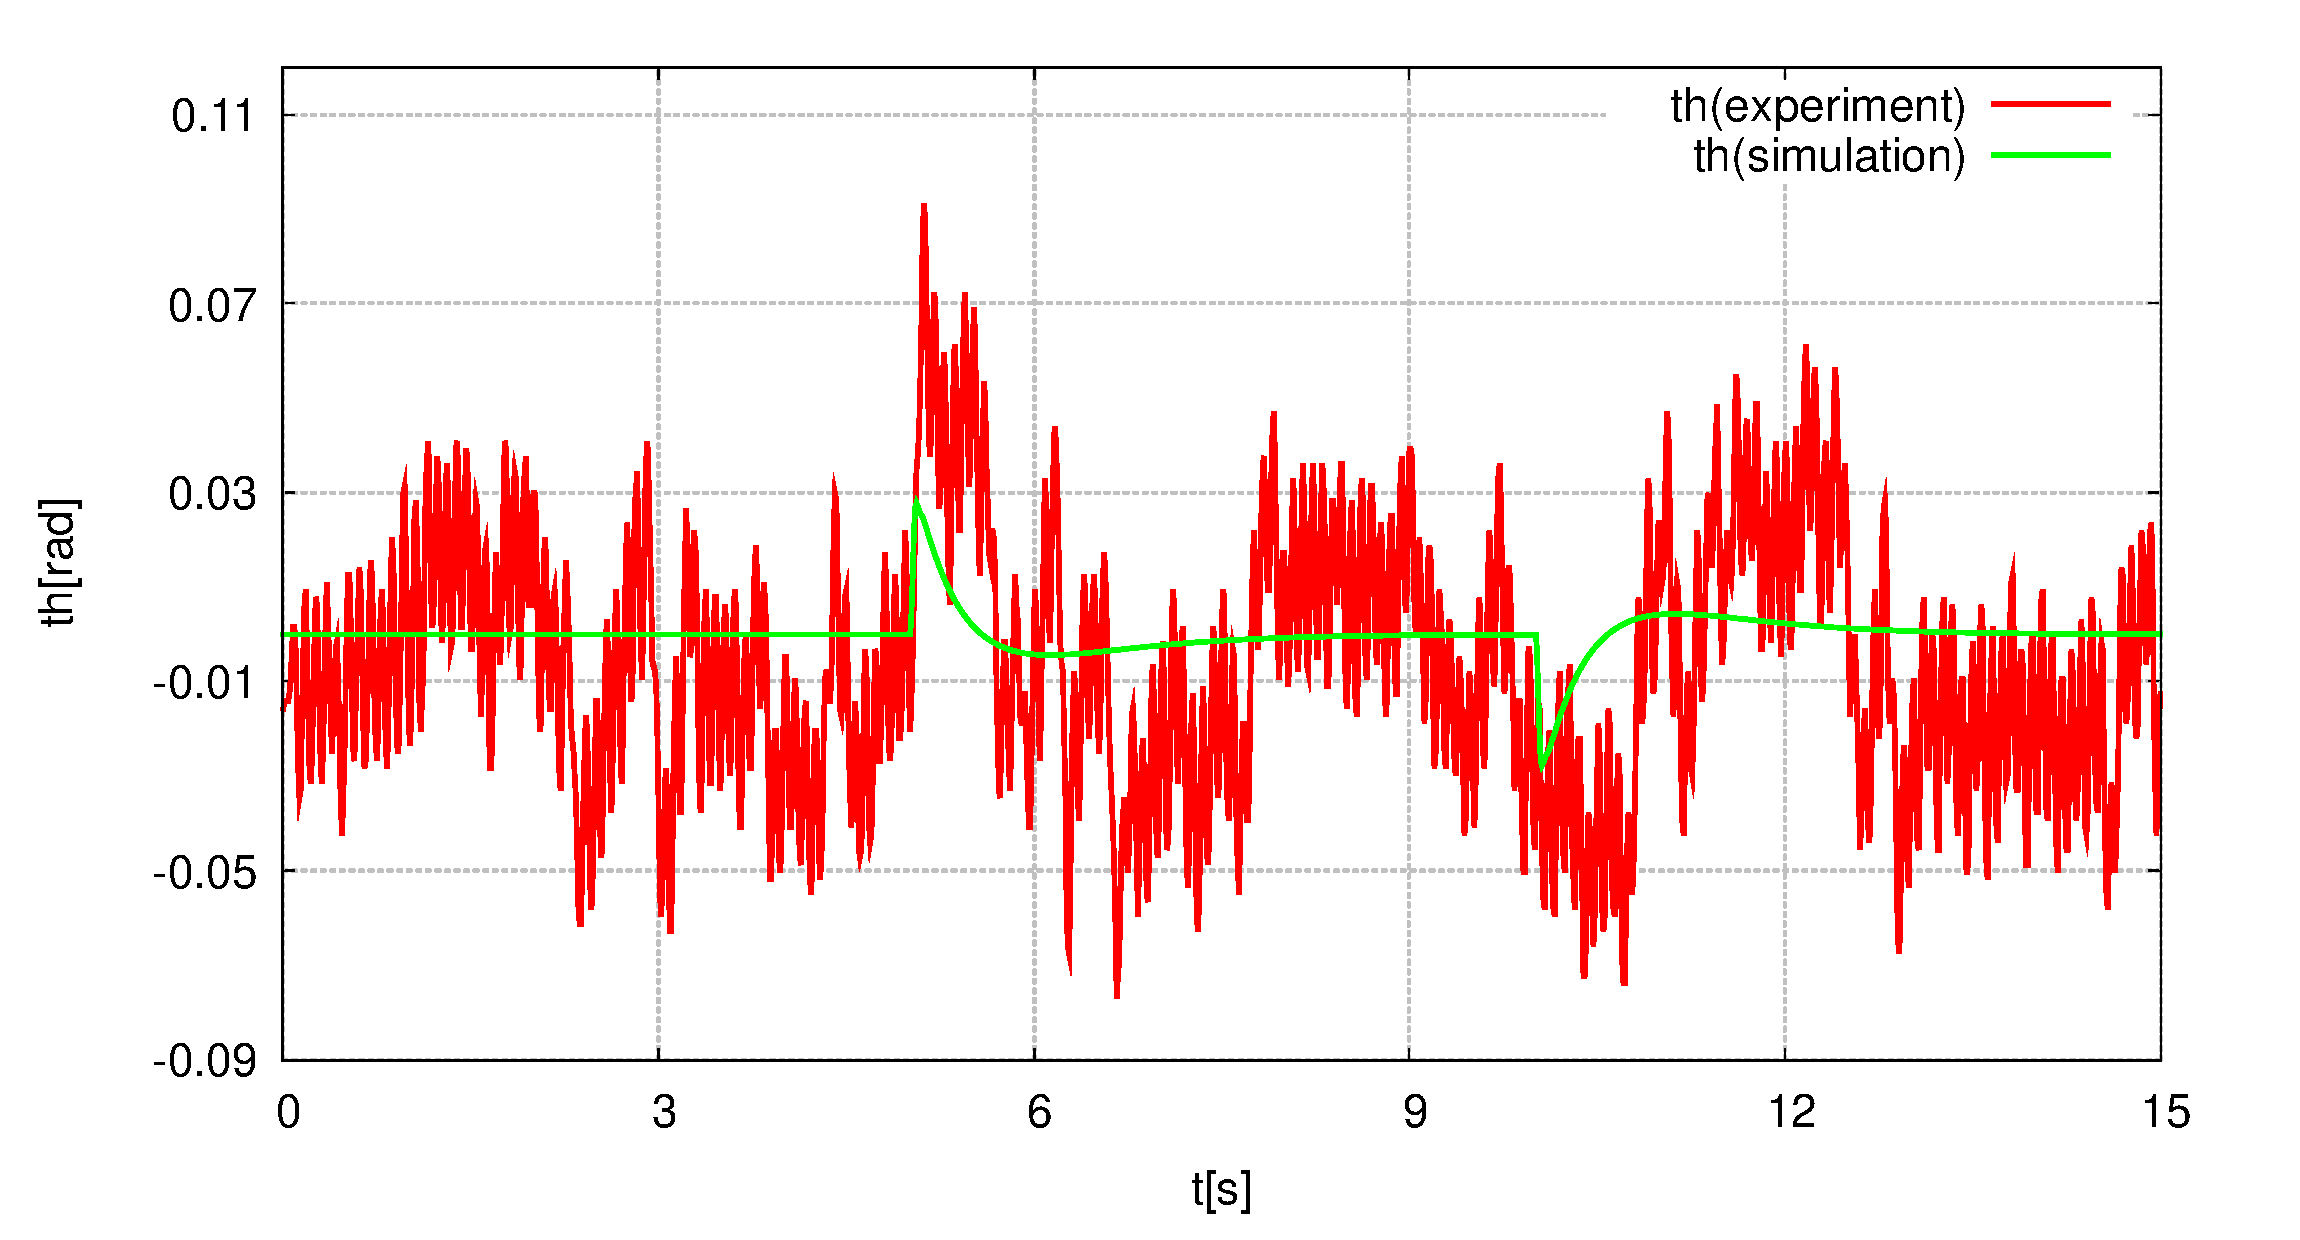
\includegraphics[width=0.49\linewidth]{gazo/experiment_Q56obs60dt10TH2.eps}
		\caption{比較結果その11(左図がr,右図が$\theta$)}
		\label{image:sono11}
	\end{figure}
	\begin{figure}[H]
		\centering
		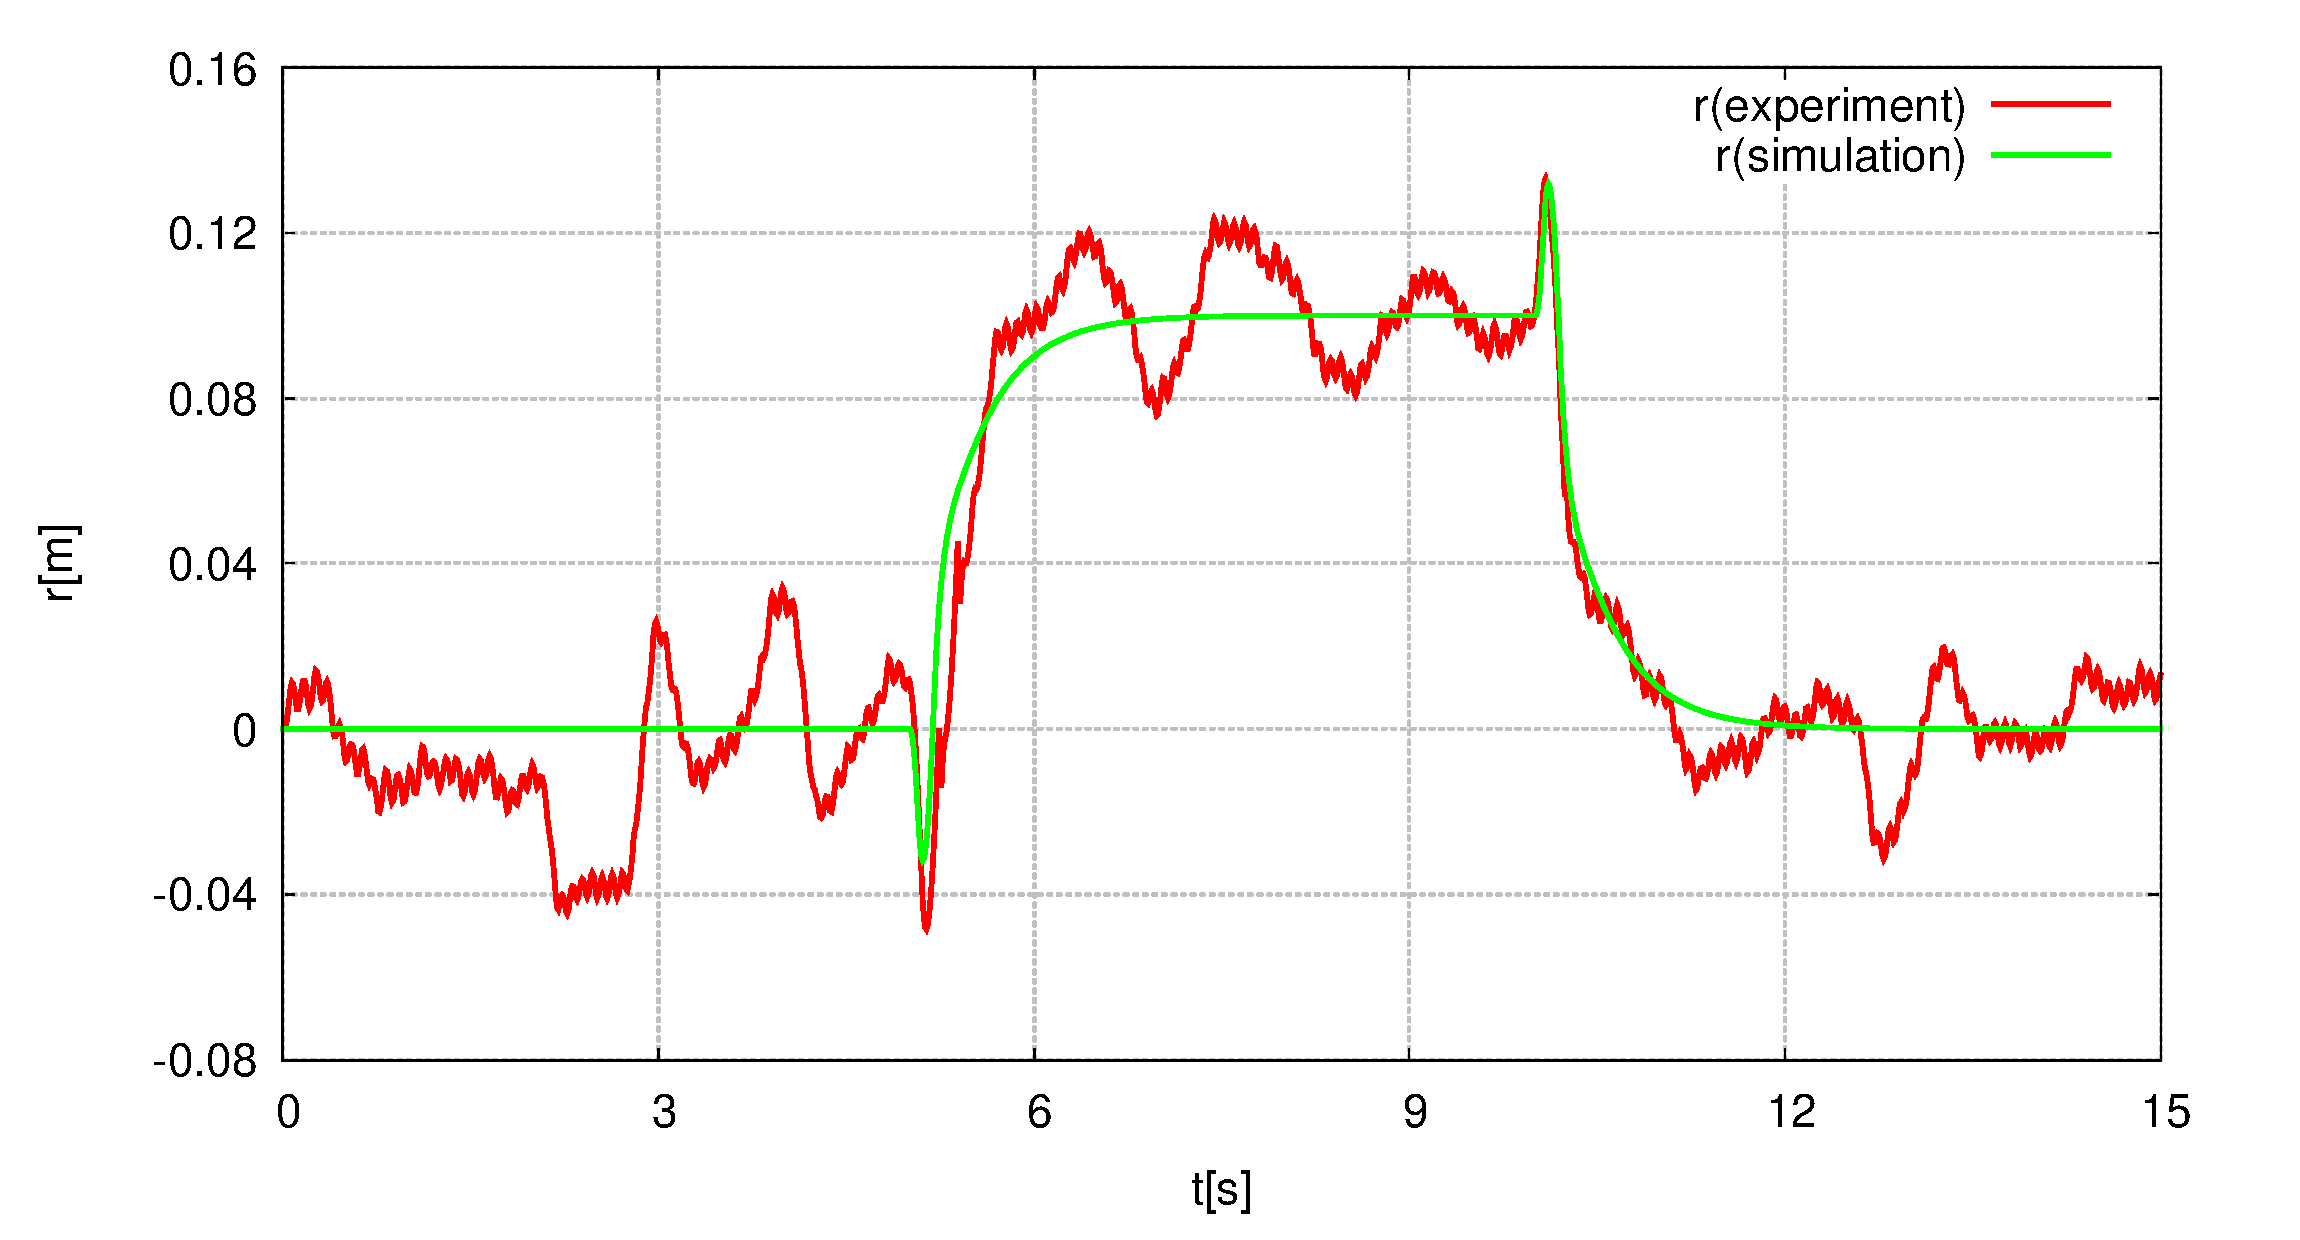
\includegraphics[width=0.49\linewidth]{gazo/experiment_Q65obs60dt10R2.eps}
		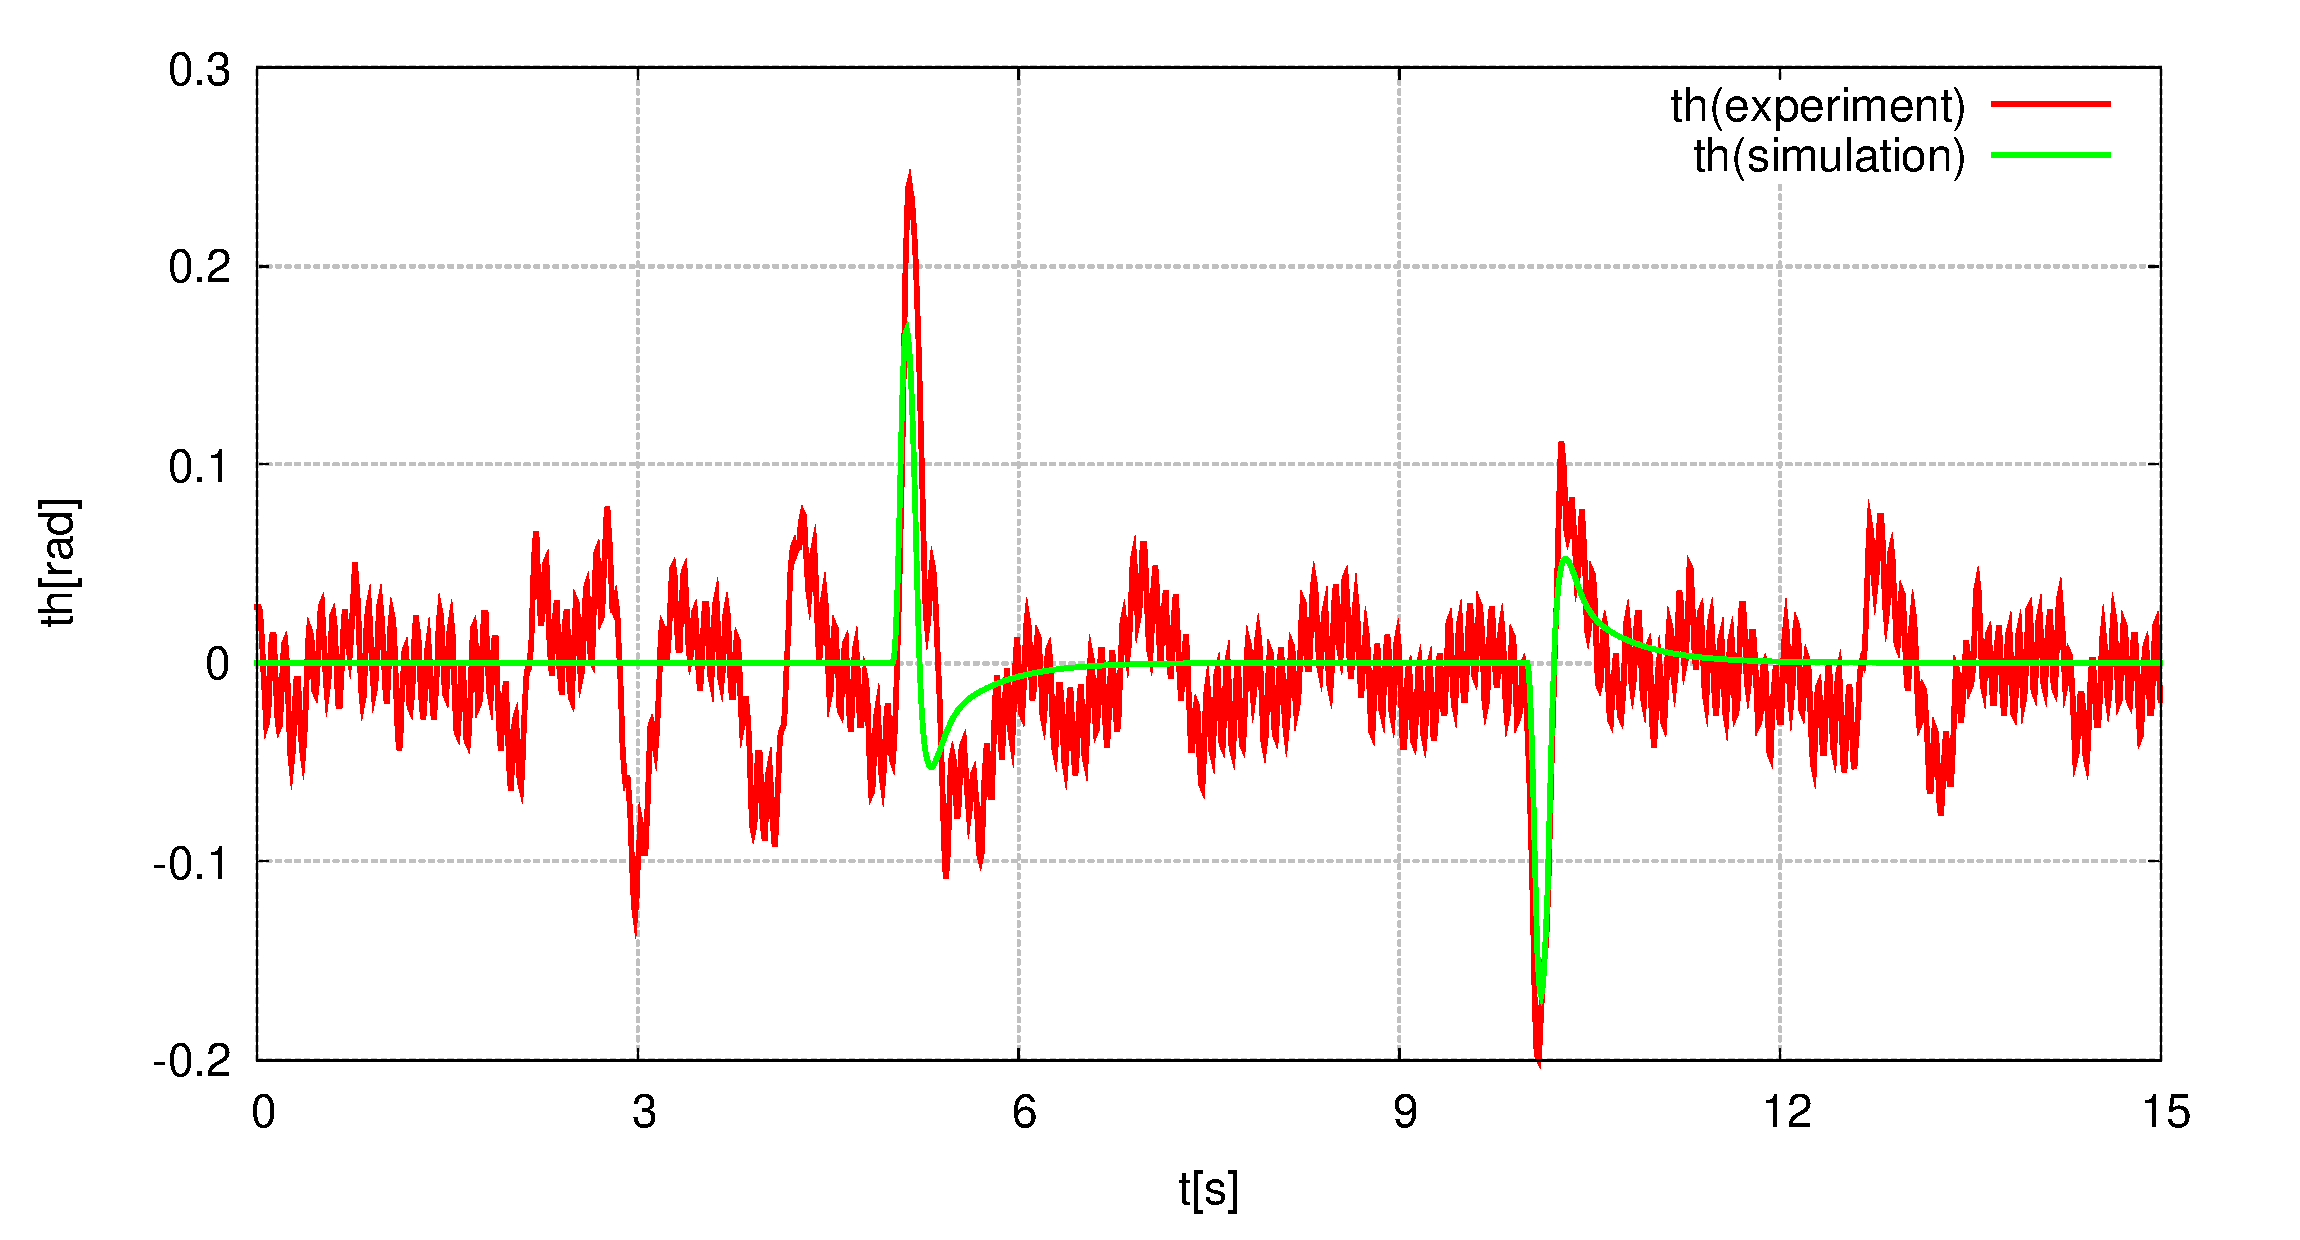
\includegraphics[width=0.49\linewidth]{gazo/experiment_Q65obs60dt10TH2.eps}
		\caption{比較結果その12(左図がr,右図が$\theta$)}
		\label{image:sono12}
	\end{figure}
	以上の図を見てみるとすべての図においてノイズがひどいが、比較的シミュレーション結果とほぼ一致している図とほとんど一致していない図があるのが分かる。
	前者に当てはまる図は図\ref{image:sono1}、図\ref{image:sono3}、図\ref{image:sono4}、図\ref{image:sono6}
	、図\ref{image:sono7}、図\ref{image:sono9}、図\ref{image:sono12}。後者に当てはまる図は、
	図\ref{image:sono2}、図\ref{image:sono5}、図\ref{image:sono8}、図\ref{image:sono11}である。
	後者に共通する特徴は重み行列が$\rm{diag}(1E5,1E6,1,1)$となっている点である。
	このようにしたときの特徴としてはシミュレーションの章でも述べたが、大きくした成分に対応する状態の応答がよくなるというものであった。
	つまり、この重み行列のとき$\theta$の応答がよくなりるはずである。
	だが、実際の図を見てみると$\theta$の応答はシミュレーションと比較しても一致しているとは言えない。
	また、$r$に関しては図を見る限りでは目標値変更に追従できていないといえる。
	これは、重み行列をこのようにしたことで状態のバランスが崩れ、$r$の応答が遅くなったためといえる。
	普通であれば、プログラムが5秒おきに目標値を変更するので、台車はその目標値に向かって動き出す。
	しかし、$r$の応答が遅いため台車は目標値に到達することができずに、プログラムから次の目標値が入力される。
	こうなってしまうことで台車は常に動き続けている状態になり、応答が良くなるはずの$\theta$もそれに伴い
	悪くなるといえる。そのため、$r$は目標値に追従できず、$\theta$の応答も悪くなってしまったといえる。
	\par
	シミュレーションと実験において差異がでたが目標値変更を行っての安定化制御を行うことができたので
	実験目的の第二項目は達成できたといえる。
	
	

%-----------------------------------------------------------
\newpage
\section{振り上げ制御及び安定化実験}
	振子を真下に配置し、そこから台車の動きだけで振子を振り上げ、
	安定化制御が可能か実験を行う(実験項目の第三項目)。
	以下に$k$を変更したときの実験結果を示す。
	\begin{figure}[H]
		\centering
		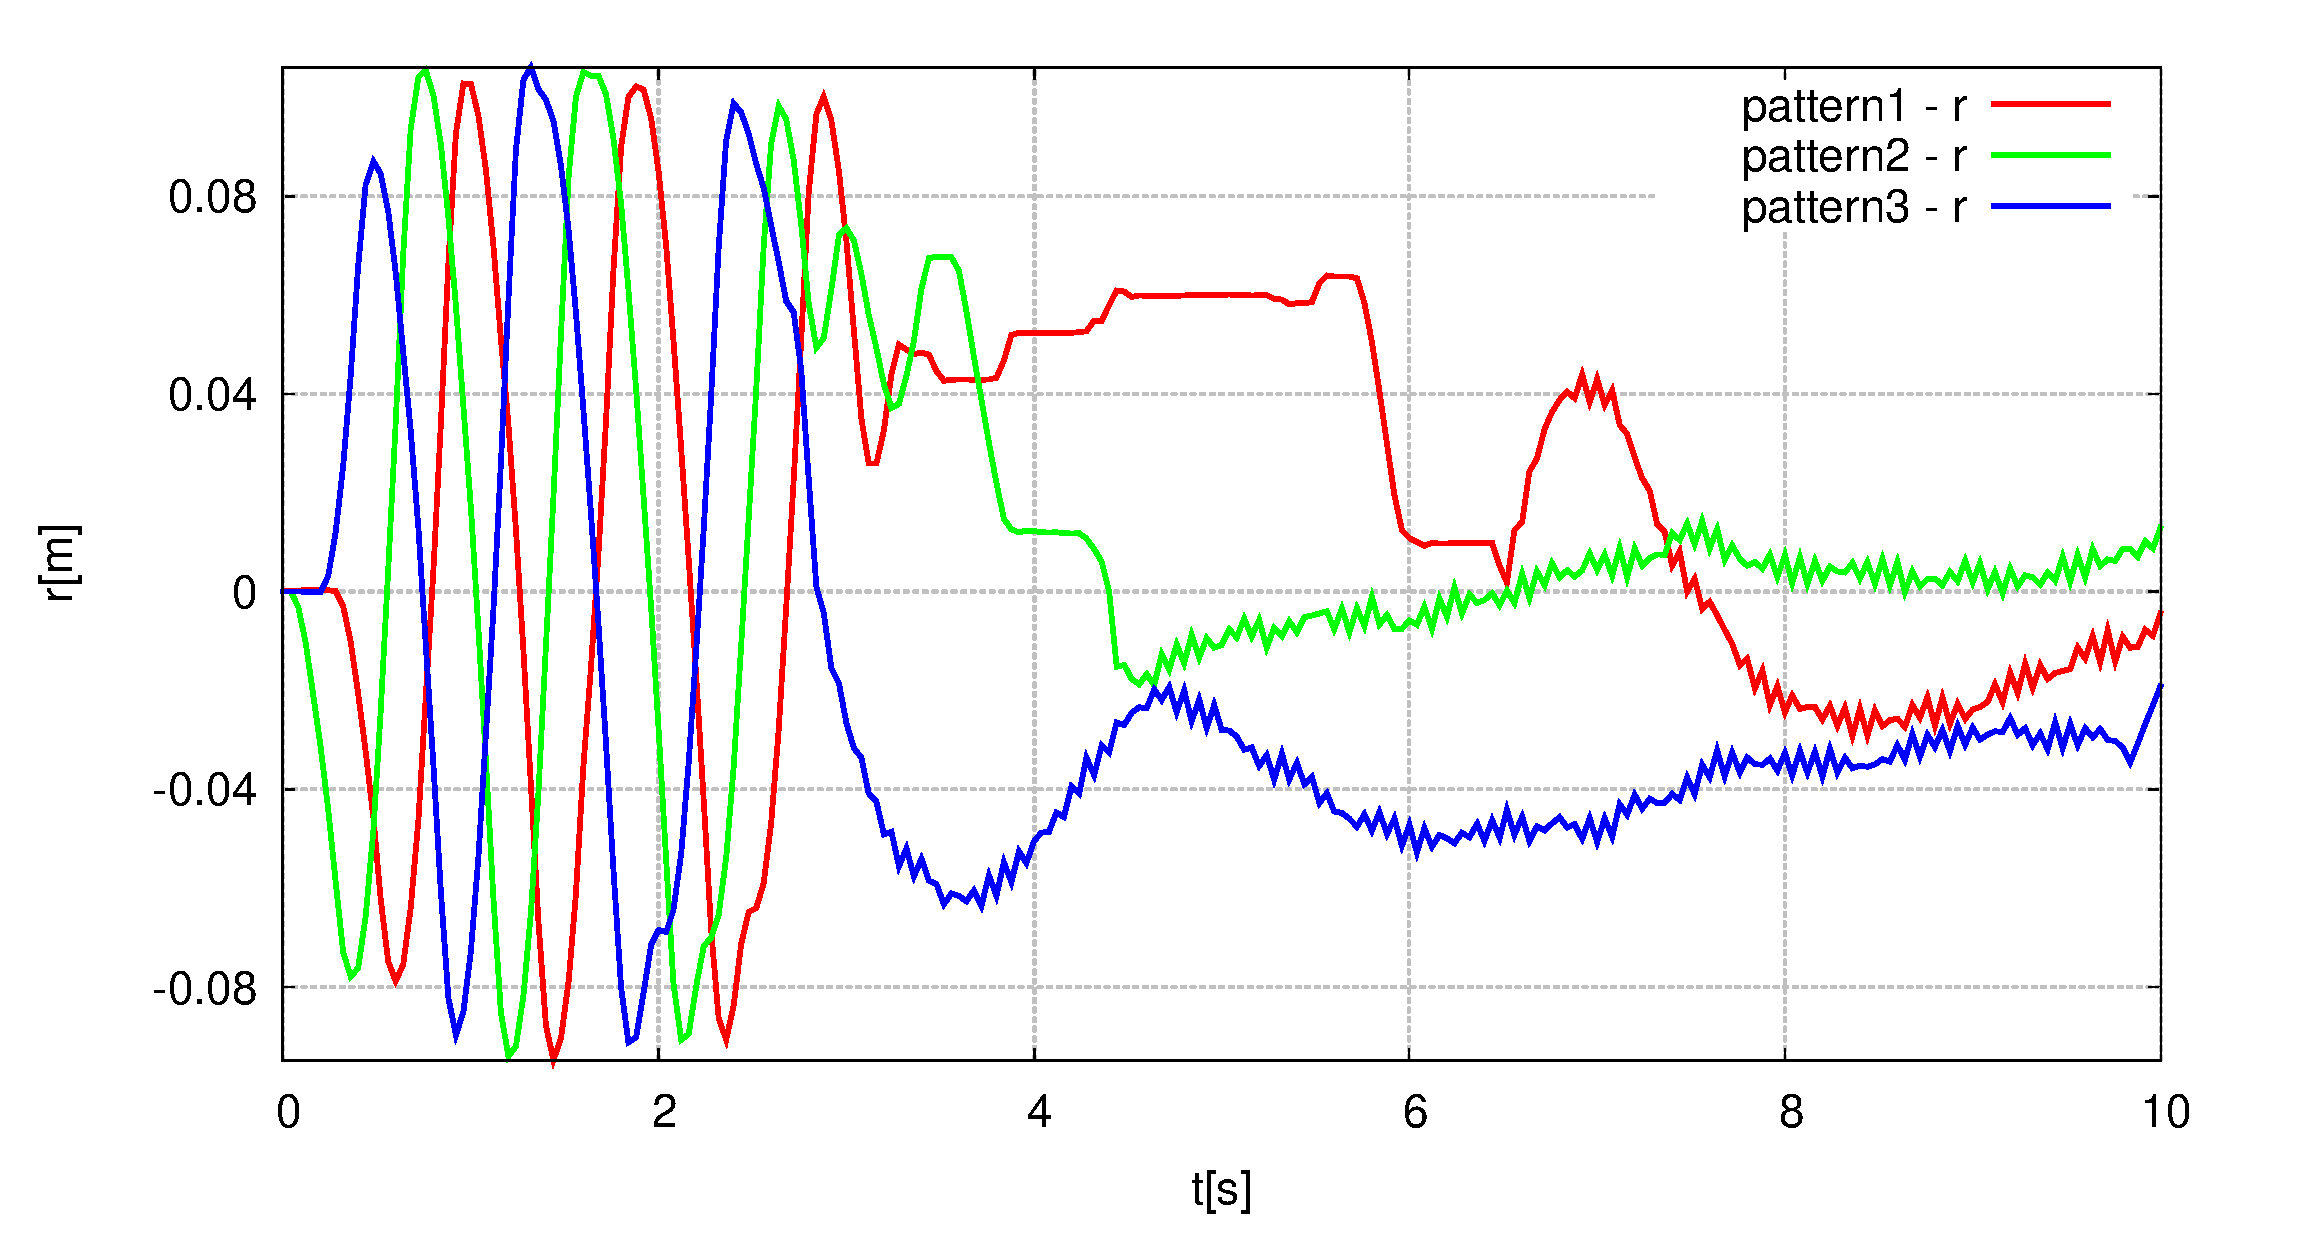
\includegraphics[width=0.49\linewidth]{gazo/Hexpe_R.eps}
		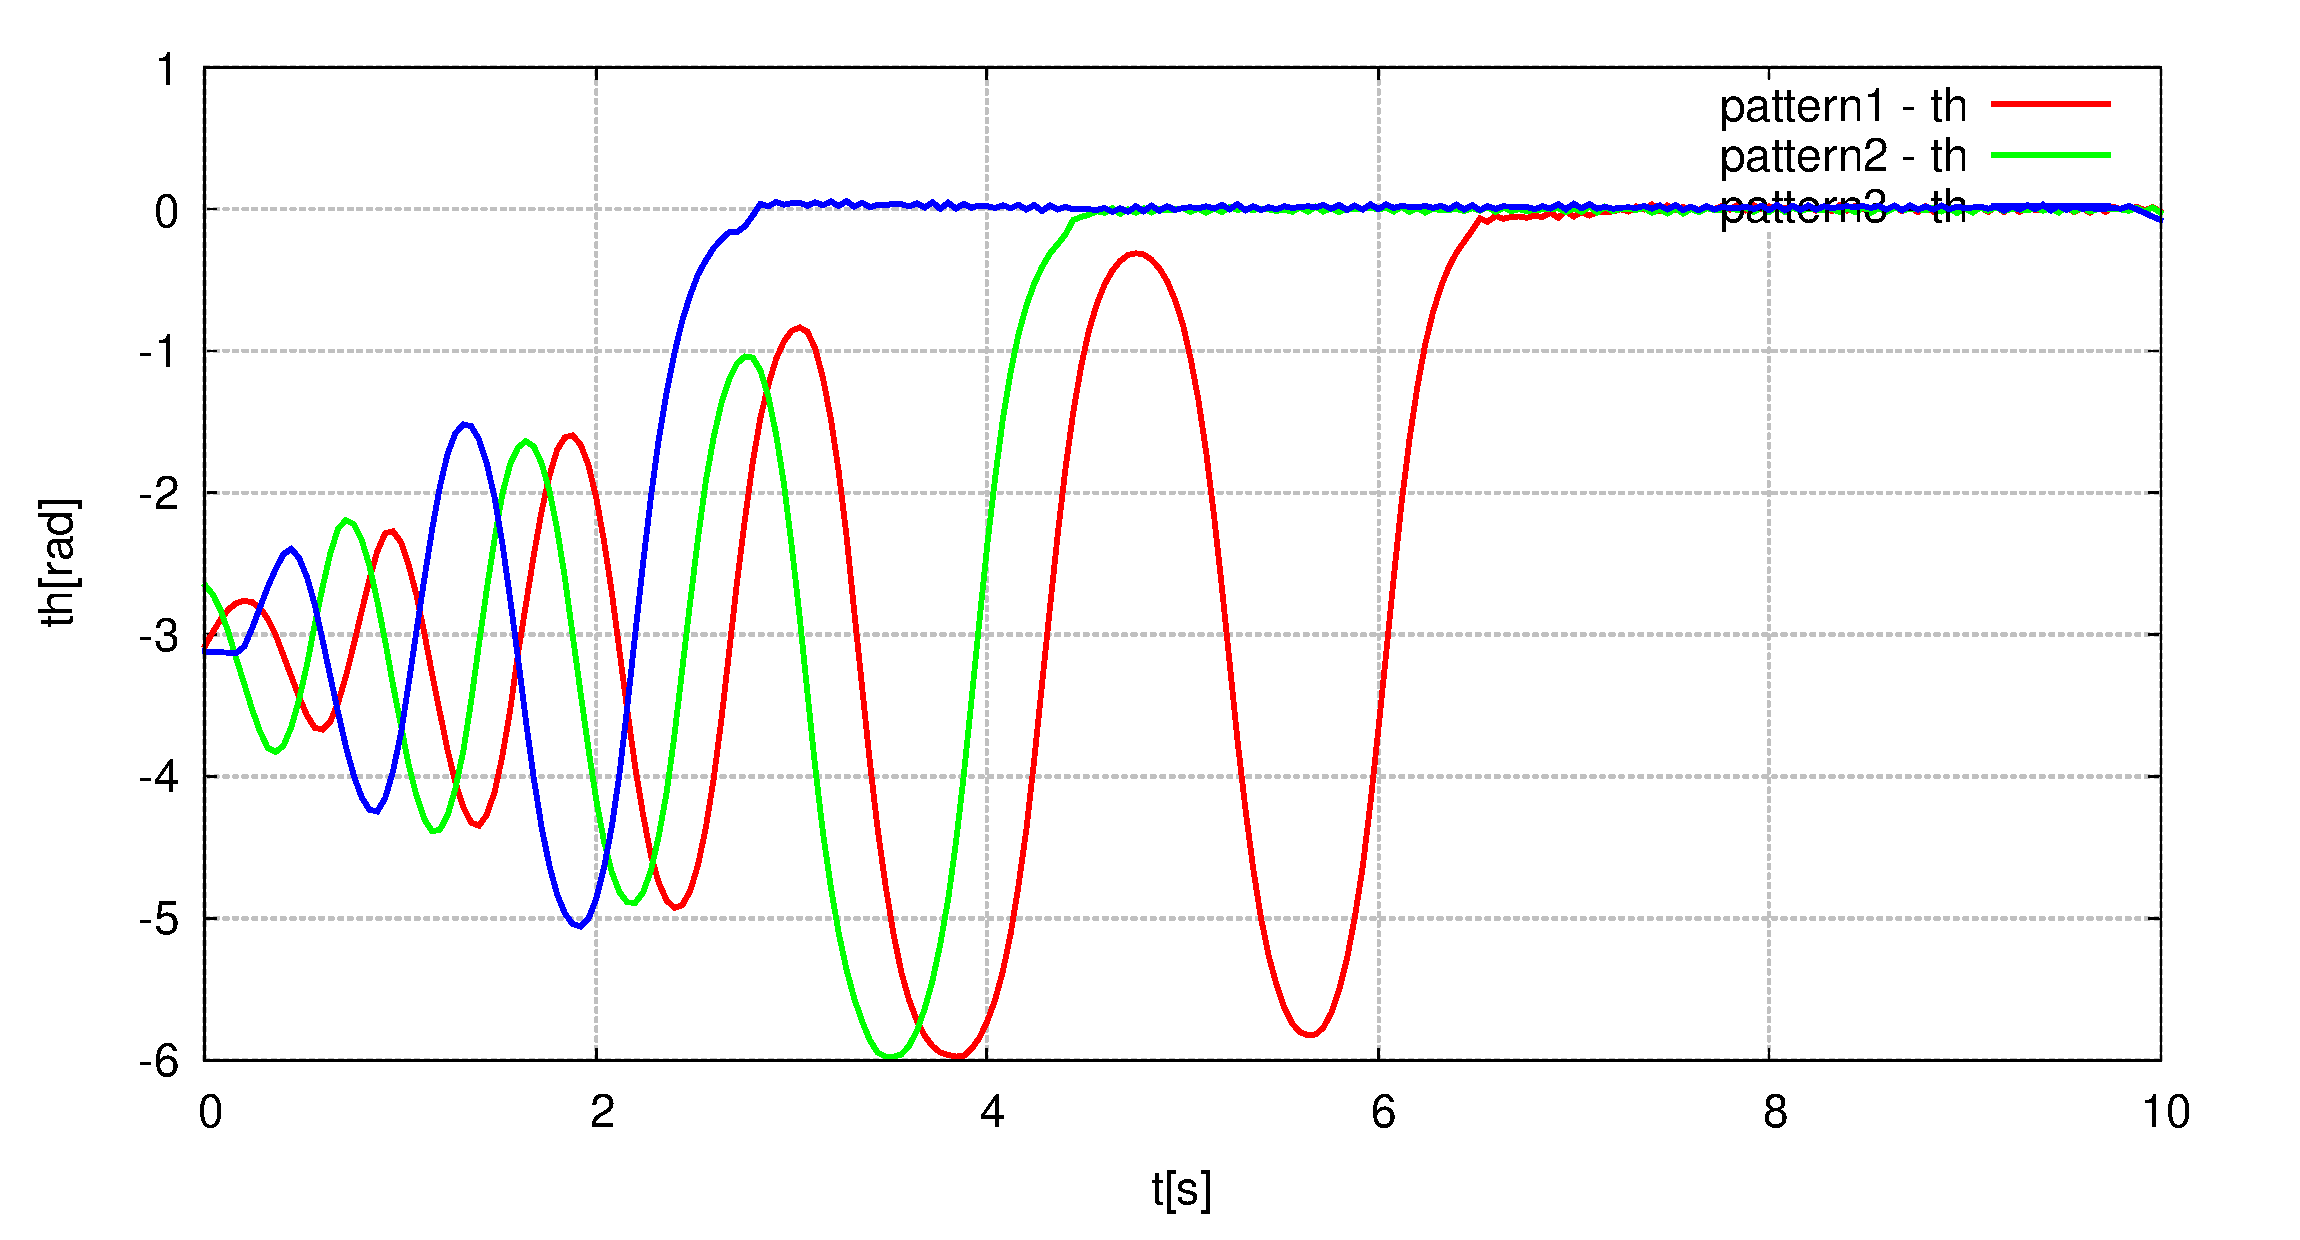
\includegraphics[width=0.49\linewidth]{gazo/Hexpe_TH.eps}
		\caption{$k$の違いによる実験結果の比較}
		\label{image:Hexpe}
	\end{figure}
	図中のPatternは以下の表に対応するパラメータである。
	\begin{table}[H]
		\begin{center}
			\caption{実験に用いたパラメータの組}
			\medskip
			
			\begin{tabular}{|c|c|c|}\hline
				& $n$ & $k$ \\ \hline\hline
				パターン1 & 0.4 & $1.0×10^3$  \\ \hline
				パターン2 & 0.4 & $1.0×10^4$  \\ \hline
				パターン3 & 0.4 & $1.0×10^5$  \\ \hline
			\end{tabular}
		\end{center}
		\label{table:huriage_huriage}
	\end{table}
	図\ref{image:Hexpe}の右図より、$k$の値が大きいほど早く安定化制御に移行していることがわかる。
	$k$が大きくなるとエネルギーの収束が早くなるため、より早く安定化制御に移行できたといえる。
	左図においても3パターンとも違う挙動を示していることがわかる。
	つまり、シミュレーションと実験では違う結果が確認されたことになる。これは、シミュレーションで用いたモデルにおいて、
	実際の倒立振子に存在する考慮すべき点を考慮していなかった可能性があるのではないかと考える。
	\par
	実験において倒立振子は机に置かれているだけと第一章で述べた。これにより台車の動きによって倒立振子自体が机の上で動くことが確認された。
	ここで確認された事象はシミュレーションでは考慮されていない点の一つであるが、ここに述べていない点についても
	考慮すべき点が存在すると考えられる。今回の目的はシミュレーションと実験結果を一致させることではないためこれ以上の言及は避けておく。
	\par
	以下に実験結果とシミュレーション結果との比較を行った図を示す。
	\begin{figure}[H]
		\centering
		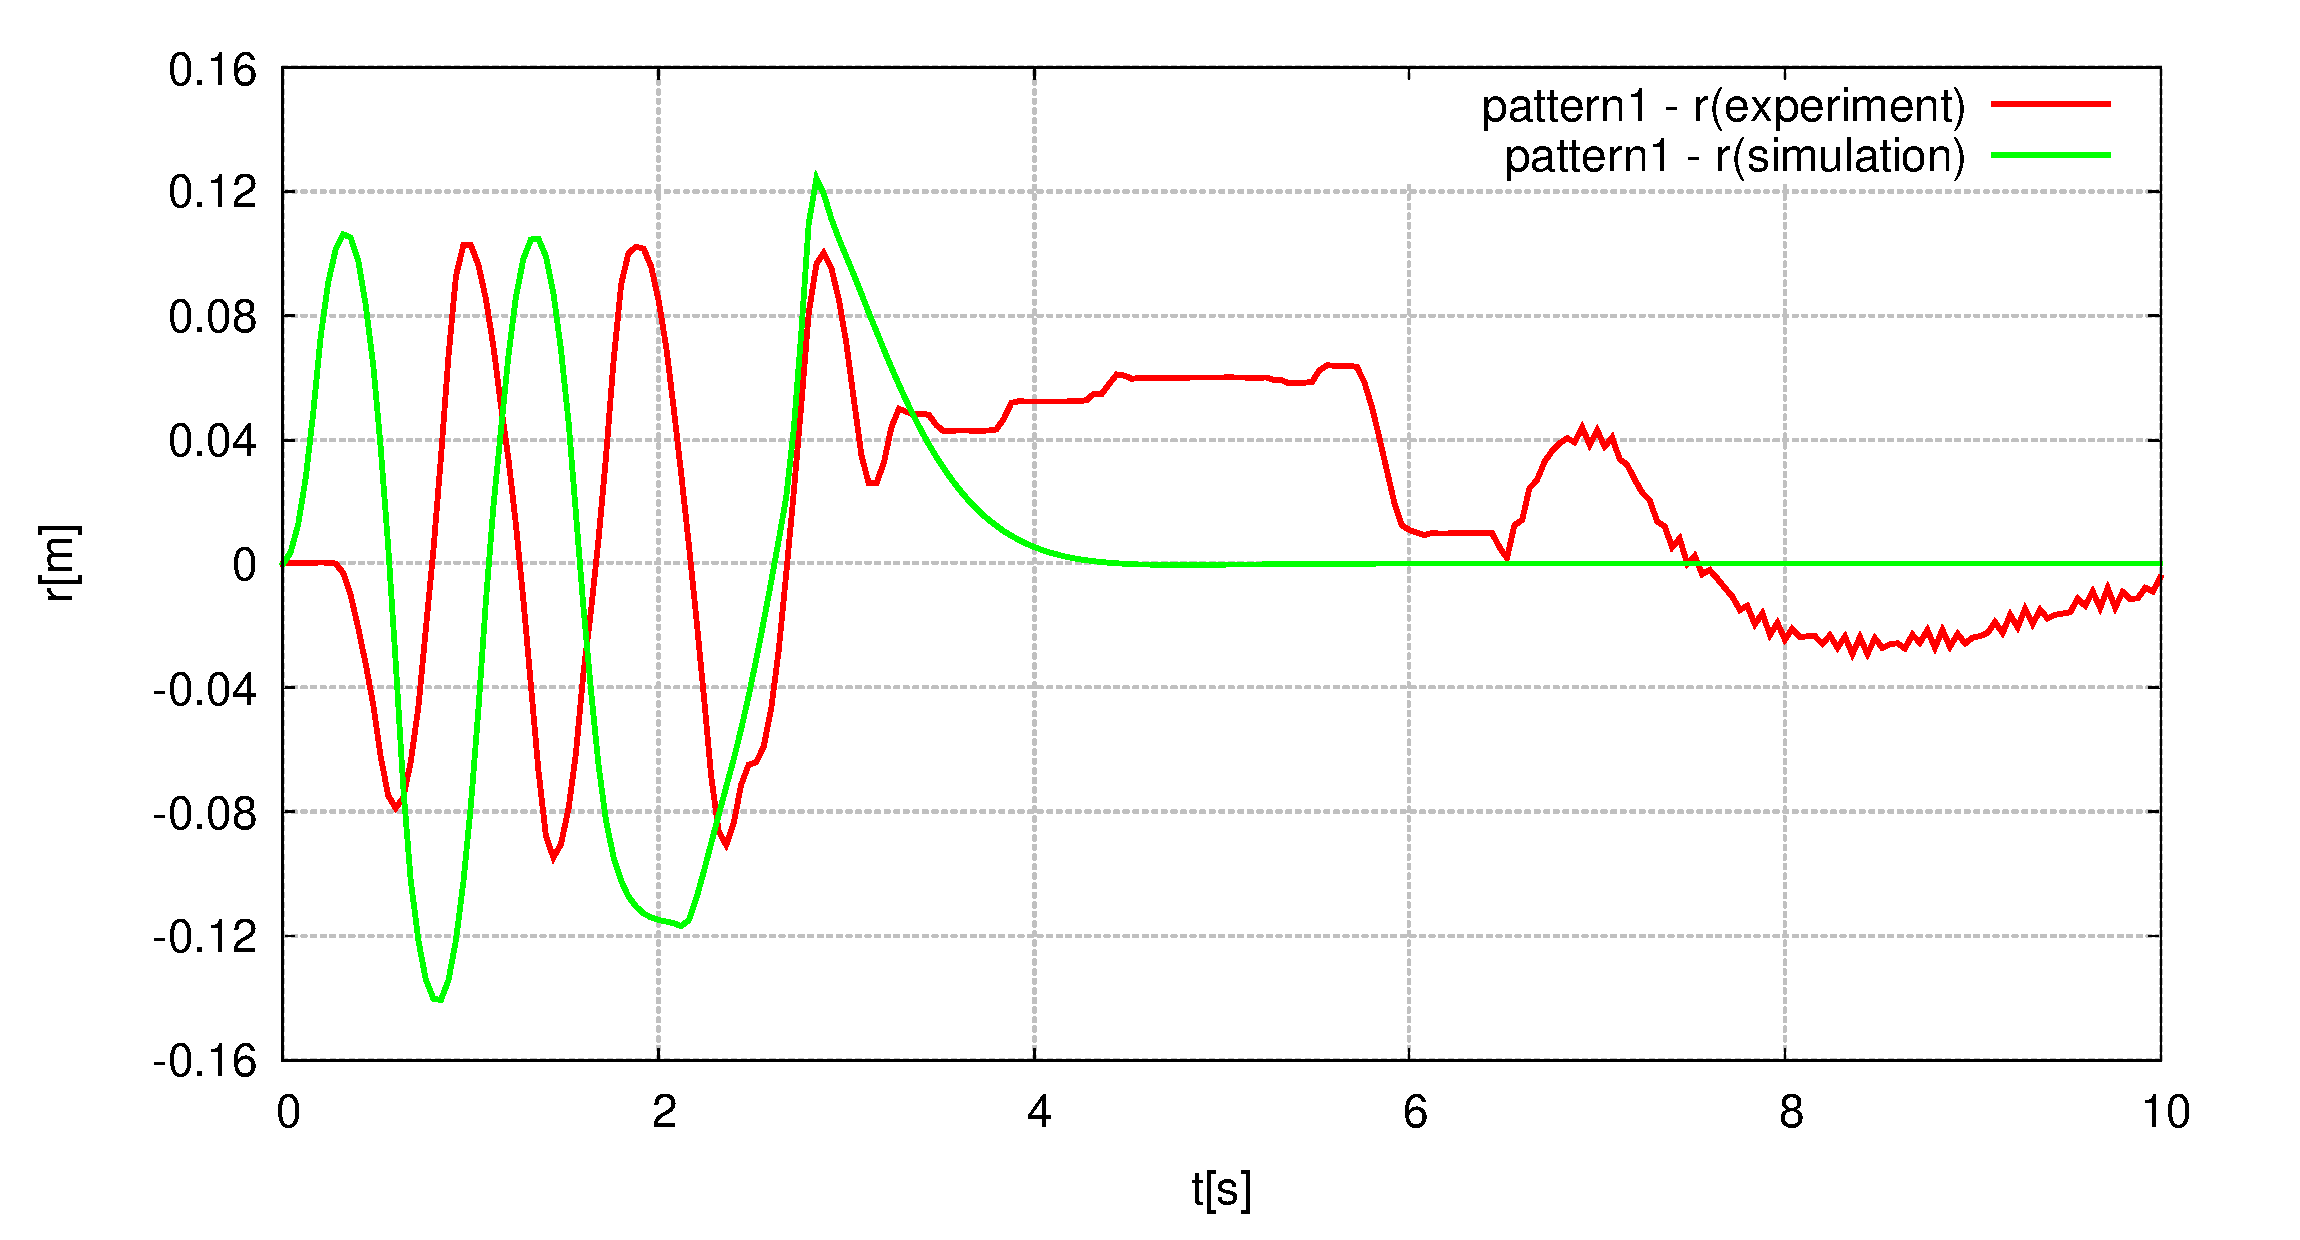
\includegraphics[width=0.49\linewidth]{gazo/HcompP1R.eps}
		\includegraphics[width=0.49\linewidth]{gazo/HcompP1TH.eps}
		\caption{比較結果(Pattern1)}
		\label{image:HcompP1}
	\end{figure}
	\begin{figure}[H]
		\centering
		\includegraphics[width=0.49\linewidth]{gazo/HcompP2R.eps}
		\includegraphics[width=0.49\linewidth]{gazo/HcompP2TH.eps}
		\caption{比較結果(Pattern2)}
		\label{image:HcompP2}
	\end{figure}
	\begin{figure}[H]
		\centering
		\includegraphics[width=0.49\linewidth]{gazo/HcompP3R.eps}
		\includegraphics[width=0.49\linewidth]{gazo/HcompP3TH.eps}
		\caption{比較結果(Pattern3)}
		\label{image:HcompP3}
	\end{figure}
	
	\par
	先ほども述べたように図\ref{image:HcompP1}、図\ref{image:HcompP2}、図\ref{image:HcompP3}からシミュレーションと実験の結果が一致していないことが確認できる。
	しかし、図\ref{image:HcompP3}の右図においては、収束角度が違うだけで、収束までにかかった時間やその挙動はほとんど同じといえる。だが、左図についてはシミュレーションと
	実験では台車の挙動に差異がみられる。この台車の動きの差異から振り子の収束角度が違ってしまったのではないかと考えられる。
	\par
	シミュレーションの結果と実験の結果に大きな違いが出てしまったが、実験において振り上げ制御から安定化制御を行うことができたので、実験目的の第三項目を達成できたといえる。
	
%-----------------------------------------------------------
\chapter{おわりに}
	本実験を通して当初の目的である、「倒立振子の安定化制御の制御系の設計を状態空間法を用いて行うことにより、線形時不変システムを設計すること」を達成できたといえる。
また、制御系のツールや数値計算ツールなどの使い方も習得することができた。

%---------------------------------------------------------------------
% 参考文献
\bibliographystyle{junsrt}
\bibliography{references}
%--------------------------------------------------------------------
% 付録
\appendix
\chapter{プログラム}
	\section{非線形モデル}
	倒立振子の非線形モデルのコードを載せる。下向きを基準としている。
	\begin{itembox}[l]{diff\_eqs}\baselineskip=1ex
		\begin{verbatimtab}[4]
Func Matrix diff_eqs(t,x,u)
Real t;
Matrix x,u;
{
	Real r,th,dr,dth;
	Matrix xp,dxp;
	Matrix K,KZ;

	r=x(1,1);
	th=x(2,1);
	dr=x(3,1);
	dth=x(4,1);

	K=[[M + m , m *l*cos(th)]
	   [m*l*cos(th) , J + m*l*l]];

	KZ=[[-f*dr+ m*l*sin(th)*dth*dth + a * u(1,1)]
		[ m*g*l*sin(th) - c*dth ]];
	
	dxp=[[x(3:4,1)][K\KZ]]; // 倒立振子の状態の微分(非線形モデル)

	cnt = cnt+1;
	XX(1,cnt) = dxp(1,1)-Xh(1,1);
	
	// 出力を更新
	return dxp;//Xは6行の行列になる
}
		\end{verbatimtab}
	\end{itembox}
%-------------------------------------------------------------------
\section{線形モデル}
	倒立振子の線形モデルのコードを載せる。下向きを基準としている。
	\begin{itembox}[l]{main.}\baselineskip=1ex
		\begin{verbatimtab}[4]

		\end{verbatimtab}
	\end{itembox}
%-------------------------------------------------------------------
\section{システム解析}
	第4章4.1節のシステム解析に用いたコードを載せる。
	\begin{itembox}[l]{main.c}\baselineskip=1ex
		\begin{verbatimtab}[4]

		\end{verbatimtab}
	\end{itembox}
%-------------------------------------------------------------------
\section{状態フィードバック}
	状態フィードバックを設計算するのに用いたコードを載せる。ただし、LQ最適制御に基づくフィードバック則とする。
	\begin{itembox}[l]{lqr}\baselineskip=1ex
		\begin{verbatimtab}[4]
Matrix A, B, Q, R, F, P;

Q = diag(1, 1, 1, 1);
R = [1];
{F,P} = lqr(A, B, Q, R);
		\end{verbatimtab}
	\end{itembox}
%-------------------------------------------------------------------
\section{最小次元オブザーバ}
	最小次元オブザーバをゴピナスの方法で計算するのに用いたコードを載せる。
	\begin{itembox}[l]{obsg}\baselineskip=1ex
		\begin{verbatimtab}[4]
CoMatrix obs_p;

obs_p = trans([(-2,0), (-2,0)]);
{Ah, Bh, Ch, Dh, Jh} = obsg(A, B, C, obs_p);
		\end{verbatimtab}
	\end{itembox}
%-------------------------------------------------------------------	
\section{コントローラの離散化}
	連続時間オブザーバを離散化するたために用いたコードを載せる。
	\begin{itembox}[l]{c2d}\baselineskip=1ex
		\begin{verbatimtab}[4]
// ここは関数の先頭
Real dt;
Matrix Ah,Bh,Jh;
Matrix Ahd,Bhd,Jhd,Hhd;

//ここはオブザーバの設計の後
dt = 0.005;
{Ahd,Hhd} = c2d(Ah, [Bh Jh], dt);
Bhd = Hhd(:,1:2);
Jhd = Hhd(:,3);
		\end{verbatimtab}
	\end{itembox}
%-------------------------------------------------------------------
\section{シミュレーション}
	第5章でシミュレーションを行ったコードを載せる。
	\begin{itembox}[l]{InPeAboveNonLinerDesign3.mm}\baselineskip=1ex
		\begin{verbatimtab}[4]
Matrix A; //システム行列
Matrix B; //入力行列
Matrix C; //出力行列
Matrix F; //状態フィードバック行列
Matrix z; // オブザーバの状態
Matrix Ah,Bh,Ch,Dh,Jh; //オブザーバに関する行列
Matrix Ahd,Bhd,Jhd;
Matrix Xh,XX,Xtest; //推定値
Real M,m,l,J,f,a,c,g,c1,c2; //パラメータ

Func void main()
{
	Real t0,t1,r0,th0,tol;
	Real dt,dtsav; //離散化に用いる変数
	Matrix x0,z0,xp0,TC,XC,UC;
	void calcParameter();
	Matrix diff_eqs(),link_eqs();
	
	t0 = 0.0; //シミュレーション開始時刻
	t1 = 18.0; //シミュレーション終了時刻
	r0 = 0; //位置の初期値
	th0 = 10.0; //角度の初期値
	x0 = [r0, th0/180*PI ,0 ,0]'; //倒立振子の初期状態'
	z = [0,0]'; //オブザーバーの初期状態'
	dt = 0.005; //サンプリング周期
	tol=1.0E-9;//許容誤差
	dtsav = 0.05; //データ保存間隔
	
	print "Now simulating\n";
	
	cnt=0; // 初期化
    calcParameter(); //シミュレーションに必要なパラメータを計算
	// Ode()によってシミュレーションを行う
	{TC,XC,UC} =
	 Ode45HybridAuto(t0,t1,dt,x0,diff_eqs,link_eqs,tol,dtsav);
	// diff_eqs() は微分方程式を記述する関数
	// link_eqs() は複数の微分方程式の関係を記述する関数。
	// TC:時間の時系列
	// XC:状態x(t)の時系列
	// UC:入出力ベクトルの時系列
	
	//数値回を表示する。横軸t, 縦軸x(t)
	mgreplot(1,TC,XC(1,*),{"r"});
	mgreplot(2,TC,XC(2,*),{"Theta"});
	
	print TC >> "TC.mat";
	print XC >> "XC.mat";
	print UC >> "UC.mat";
}



// diff_eqs() は微分方程式を記述する関数
Func Matrix diff_eqs(t,x,u)
// tは時間
Real t;
Matrix x,u;
{
	Real r,th,dr,dth;
	Matrix xp,dxp;
	Matrix K,KZ;
	
	r=x(1,1);
	th=x(2,1);
	dr=x(3,1);
	dth=x(4,1);

	K=[[M + m , m *l*cos(th)]
	   [m*l*cos(th) , J + m*l*l]];

	KZ=[[-f*dr+ m*l*sin(th)*dth*dth + a * u(1,1)]
		[ m*g*l*sin(th) - c*dth ]];
	
	dxp=[[x(3:4,1)][K\KZ]]; // 倒立振子の状態の微分(非線形モデル)
	
	cnt = cnt+1;
	XX(1,cnt) = dxp(1,1)-Xh(1,1);

    // 出力を更新
	return dxp;//Xは6行の行列になる
}



// link_eqs() は複数の微分方程式の関係を記述する関数。
Func Matrix link_eqs(t,x)
Real t;
Matrix x;
{
    Matrix u;
    Matrix xref;
	Matrix xh,y;

    //台車の可動範囲に関する制限
    if (x(1,1) <= -0.16 || 0.16 <= x(1,1)) { // r=x(1,1)
    	OdeStop();
    }
	
	y = C*x; // 出力の計算
	xh = Ch*z + Dh*y; // 状態の推定値
	Xh= xh; //推定値を保存
	xref = [0,0,0,0]'; // 状態の目標値'
	if(0<=t && t<=5){
		xref = [0,0,0,0]'; // 状態の目標値'
	}else if(5<t&&t<=10){
		xref = [0.1,0,0,0]'; // '
	}else if(10<t&&t<=15){
		xref = [0,0,0,0]'; // '
	}
    u = F*(xref - xh);

    //入力の大きさに関する制限
    if(u(1,1) <= -15) {
        u(1,1) = -15;
    }else if (u(1,1) >= 15) {
        u(1,1) = 15;
    }

	z = Ahd*z + Bhd*y + Jhd*u; // オブザーバの状態更新
    
    //入力を更新
    return u;
}

Func void calcParameter(){

    CoMatrix pc,obs_p;
    Matrix A21,A22,B2,K,N;
	Matrix Ah ,Bh ,Jh ; // 連続時間オブザーバの係数行列
	Matrix Hhd; // 離散時間オブザーバの係数行列
	Real dt; //サンプリング周期
	Matrix Q,R,P;

    

    //物理パラメータの設定
	M=0.69;   m=0.031; l=0.15;
	J=2.5E-4; f=7.6; a=0.61;
	c=5.4E-5; g=9.8; c1=1.0;
	c2=1.0;

    // システム行列Aの準備
    K=[[M+m,m*l][m*l,J+m*l^2]];
	A21 = K~*[[0,0][0,m*g*l]];
	A22 = K~*[[-f,0][0,-c]];
	A=[[Z(2),I(2)][A21,A22]];

    //入力行列Bの準備
	B2 = K~*[[a][0]];
	B=[[Z(2,1)][B2]];

	//出力行列Cの準備
    N=[[c1,0][0,c2]];
    C=[N,Z(2)];

	//状態フィードバック行列Fを準備する
    //pc=[(-100,0),(-50,0),(-1,0),(-1,0)]'; 閉ループ系の極'
    //F = pplace(A,B,pc);
	
	//LQ最適制御のための状態フィードバック行列Fの準備
	Q = diag(1E5,1E5,1,1);
	R = [1];
	{F,P} = lqr(A, B, Q, R);

	//ゴピナスの方法で最初次元観測器を設計する
	obs_p = trans([(-30,0), (-30,0)]); // オブザーバの極
	//read obs_p; // 極を編集する
	{Ah, Bh, Ch, Dh, Jh} = obsg(A, B, C, obs_p); // ゴピナスの方法による設計

	// 連続時間オブザーバをサンプリング周期で離散化
	dt = 0.005;
	{Ahd,Hhd} = c2d(Ah,[Bh, Jh], dt); //離散化
	Bhd = Hhd(:,1:2); //係数行列の取り出し
	Jhd = Hhd(:,3); // 係数行列の取り出し
}
		\end{verbatimtab}
	\end{itembox}	
%-------------------------------------------------------------------
\section{安定化制御及び目標値変更実験}
	安定化制御及び目標値変更実験を行うために使用したコードを載せる。
	\begin{itembox}[l]{sample.mm}\baselineskip=1ex
		\begin{verbatimtab}[4]

		\end{verbatimtab}
	\end{itembox}
%-------------------------------------------------------------------
\section{振り上げ制御及び安定化実験}
	振り上げ制御及び安定化実験を行うために使用したコードを載せる。
	\begin{itembox}[l]{sample.mm}\baselineskip=1ex
		\begin{verbatimtab}[4]

		\end{verbatimtab}
	\end{itembox}
%-------------------------------------------------------------------

\end{document}